\chapter{Signal optimisation and extraction}
\label{chap:ayield}
\minitoc
\myepigraph{What I would recommend to them is, if they have some idea
  -- however crazy it is -- they should check up on it. Once in a
  hundred times it will turn out to be a good idea.}{Simon van der Meer}
\externaldocument{pQuarkonia}

\section{Preamble}
\label{sec:preamble}
\subsection{Analysis strategy}
\label{subsec:strategy}
Our goal is to understand \PgU\ modification and
suppression in heavy ion collisions, to the largest possible extent. We have
seen in the introductory chapters that the most prominent signature of
deconfinement is quarkonium melting; Moreover, this melting is
thought to be sequential, with the looser bound states diluting into
the plasma before the tighter ones, as the energy density increases.


The simplest way to investigate the sequential melting of quarkonium
states is to look at the individual yields recorded in centrality
classes. A first measurement of the centrality dependence of \PgU\ suppression has been presented in
% Chapter~\ref{chap:pquarkonia}, 
Figure~\ref{fig:hinupsilonsraa}, page~\pageref{fig:hinupsilonsraa}. This
measurement made use of the nuclear modification factor:

\begin{equation}
\RAA = \frac{N^{\textrm{PbPb}}}{\TAA \; \sigma_{pp}},
\label{eq:raa1}
\end{equation}  

where $N^{\textrm{PbPb}}$ is the measured rate of the process of interest in
PbPb collisions, and \TAA\ is the average nuclear overlap for a given impact parameter (or centrality) range. This gives a
normalised yield directly comparable to the $pp$ cross section, $\sigma_{pp}$,  for the particle of interest.

When \RAA\ is equal to unity, it means that the rate
observed for a particle produced in PbPb is strictly equal to that of a superposition of incoherent $pp$ collisions, indicating that the particle rate does not suffer from
nuclear or plasma effects. This is for example the case with electroweak probes
$W^{\pm}$ and $Z^{0}$, and high-\pt photons. One should be very
careful however as in many cases the \RAA\ can suffer from
several effects that add up or compensate themselves. 
% This happens with particles that are known to suffer from nuclear effects. 
One infamous example
being the interplay between \Jpsi\ suppression and regeneration,
that compensate to produce a flat \RAA\ over a wide centrality range~\cite{jpsiALICE}.

\subsection{First observations motivating newer measurements}
\label{subsec:firstobs}

For Figure~\ref{fig:hinupsilonsraa},
the \RAA\ was computed for \PgUa\ and \PgUb\ in seven bins of
increasing centrality, using PbPb data of 2011 ($\mathcal{L} = \; 150
\;\invmub$) and $\mathcal{L}_{pp} = 230 \;
\invnb$ of $pp$ data at the same center of mass energy, \s\ = \snn\
= 2.76 \TeV. We have seen that \PgUb\ is consistently more suppressed
than \PgUa: this is one reason to believe that suppression is sequential. 
However, in the simple hypothesis of sequential melting
occurring to the full, one would expect the onsets of the \PgUb\ and \PgUa\ suppressions to coincide, which was apparently not the case in this data. 

Another popular belief is that either one of the quarkonium
states -- dissociating or not -- may escape the PbPb interaction
without suffering from colour screening (cause for melting) if they have sufficient momentum. In this frame of
ideas, high-\pt\ quarkonia may survive, and the \RAA\
should depend on \pt. This could also explain the \PgUb\ being
non-zero in central events. The following Figures~\ref{fig:raarap2010} left and
% \ref{fig:raapt2010} 
right present the first attempt to measure the kinematical dependences of the \PgU(1S)~\cite{torsten}, motivating further the analysis presented here. 

\begin{figure}
\begin{center}
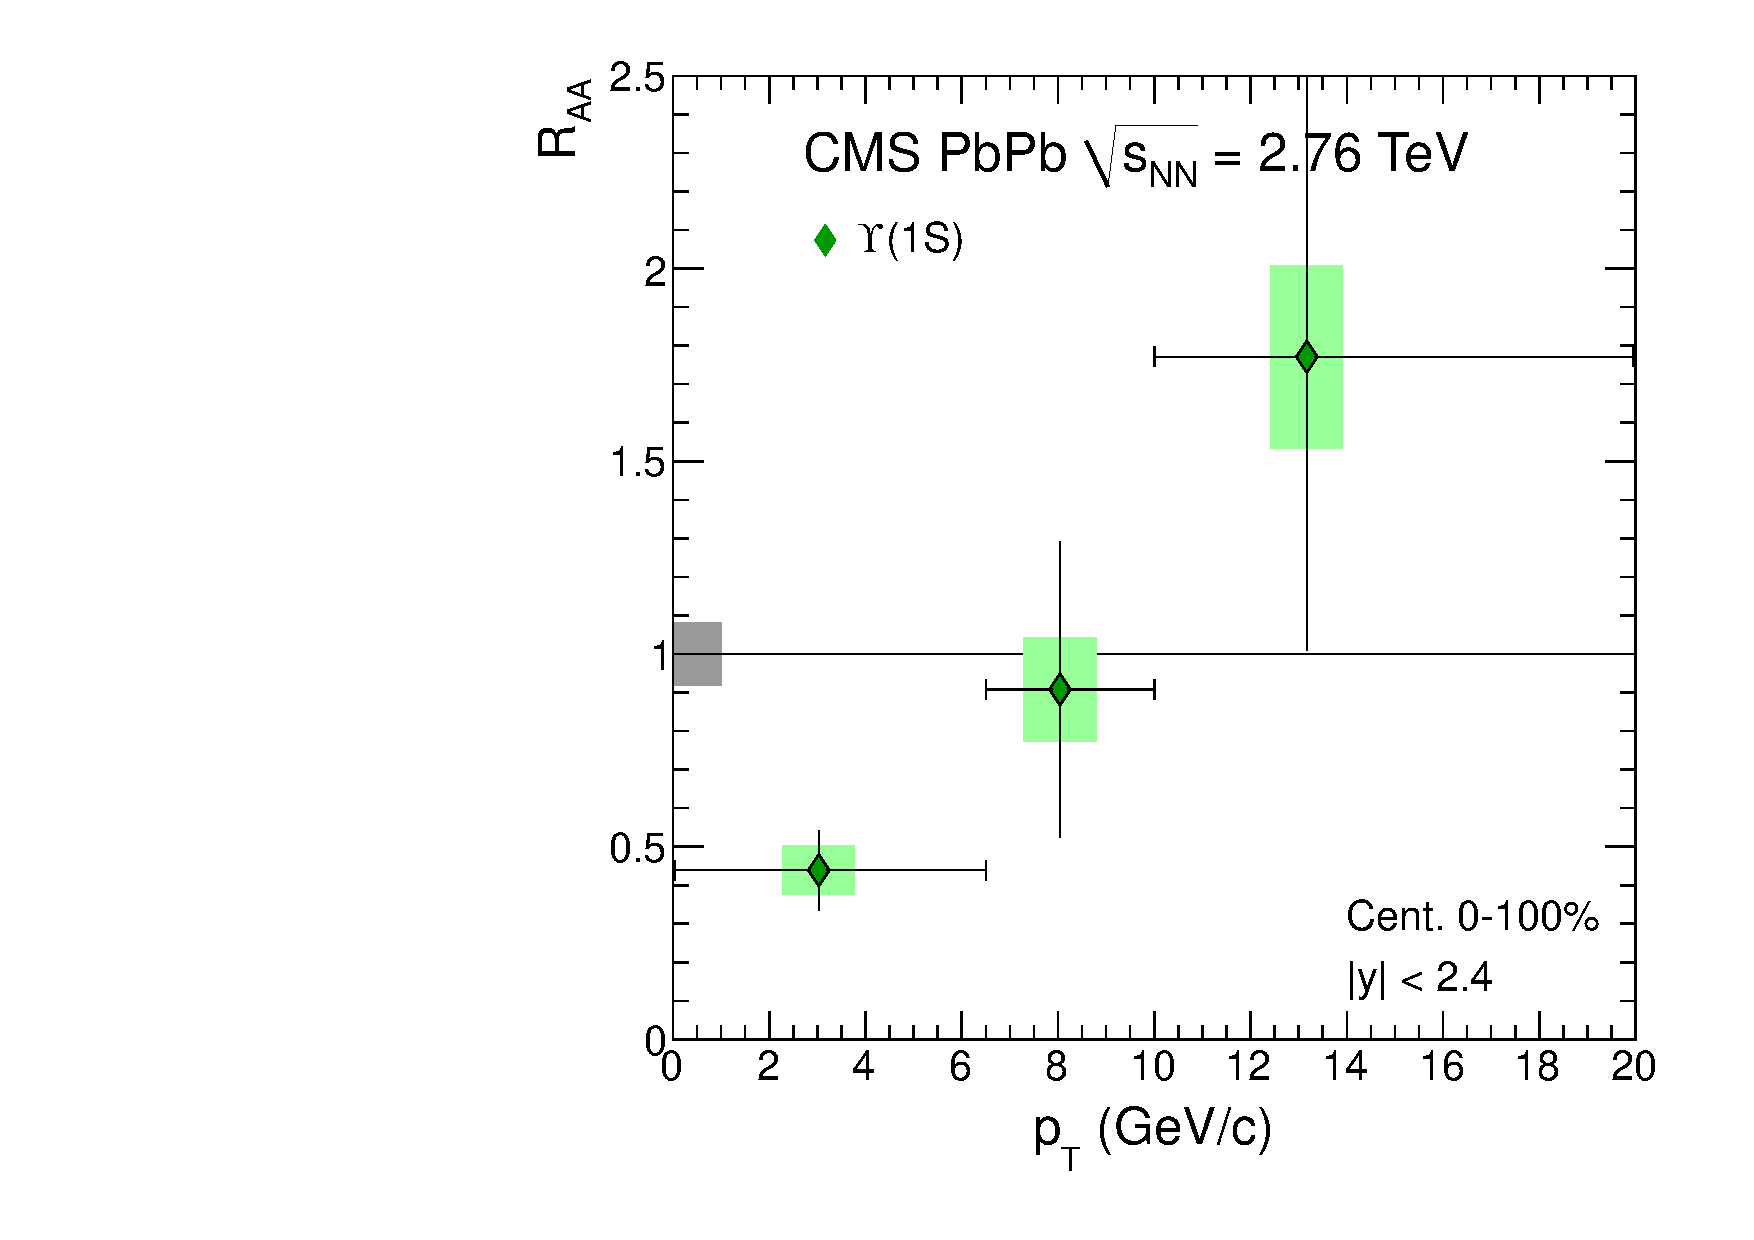
\includegraphics[width=0.43\textwidth]{Chapters/aYield/upsilon_RAA_pt.pdf}
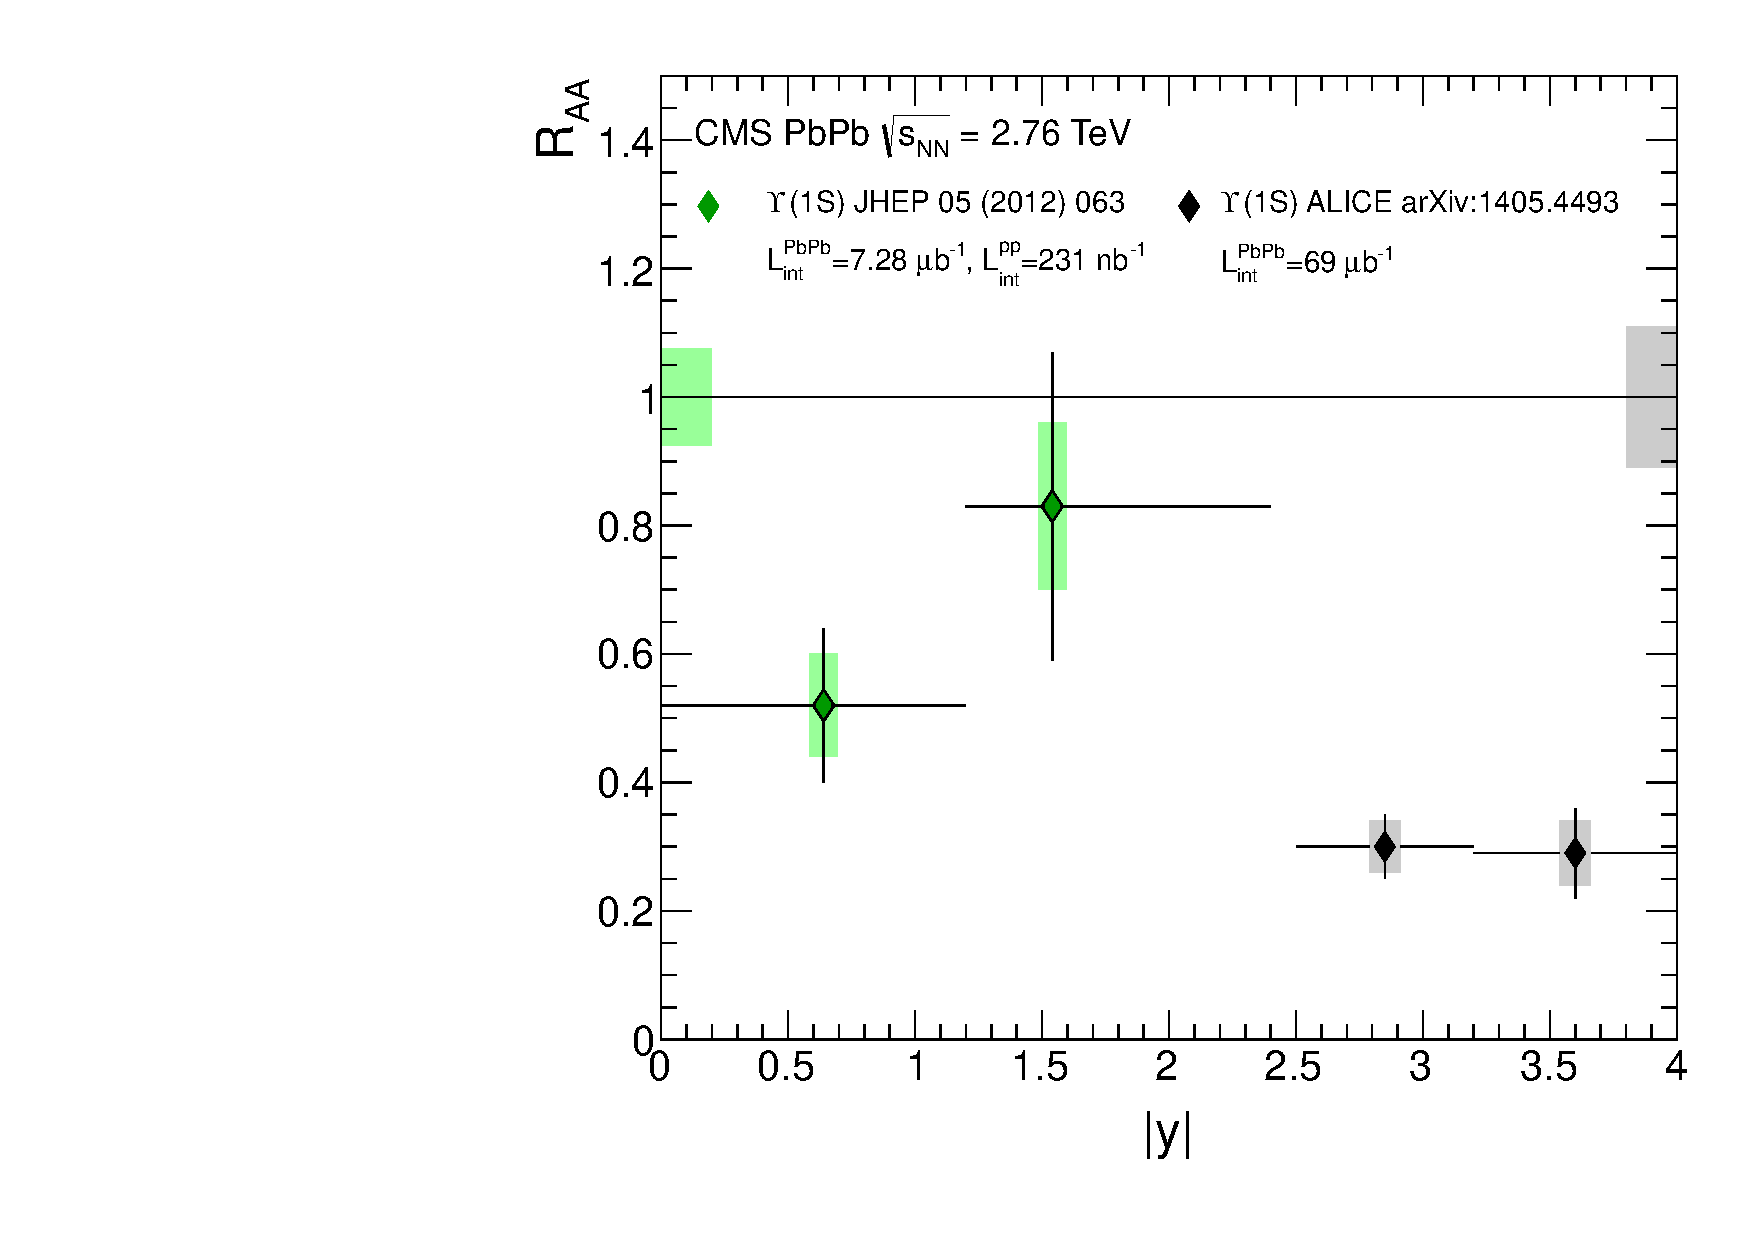
\includegraphics[width=0.42\textwidth]{Chapters/aYield/Raa_Y1S_rap_CMSaliceFinal.pdf}
\caption{Nuclear modification factor \RAA\ of \PgUa\ in PbPb, measured
  with 2010 CMS data ($\mathcal{L}_{\rm PbPb} = 7.28
\; \invmub$, $\mathcal{L}_{pp} = 230
\; \invnb$). Left: transverse mometum dependence. The high-\pt points, albeit of poor significance, seem to
exhibit less suppression than low-\pt\ ones. From~\cite{torsten}. Right:
Rapidity dependence, compiling also ALICE data from~\cite{ALICEUpsilonHI}.} 
% Personal compilation for Scomparin~\cite{scomparinlhcp2014}.}
\label{fig:raarap2010}
\end{center}
\end{figure}

In Figure~\ref{fig:raarap2010} (left), the \PgUa\ is obviously suppressed at low-\pt, with
increasing \RAA\ (i.e. less suppression) when the transverse momentum of the \PgUa\
increase. At higher momenta the large statistical uncertainties prevent to reach any strong conclusion on the \pt\ dependence of the suppression. In the rapidity compilation on Figure~\ref{fig:raarap2010} (right), the CMS data at
mid-rapidity appears at tension (though again with large uncertainties) with the higher rapidity points of ALICE~\cite{ALICEUpsilonHI}, themselves exhibiting a relatively stronger suppression than CMS data overall. This would tend to indicate that the \PgU\
suppression is located at low-\pt. 

However, considering
the dissociation temperature of \PgUa\ being at least two times larger
than the deconfinement temperature, it is often thought that \PgUa\
are not `melting' in the QGP. The apparent \PgUa\ suppression would thus be
the result of the excited state suppression, and the feed-down
contributions from excited states being lost would bring the
\RAA\ of \PgUa\ down to lower values.

Unfortunately, the $pp$ and PbPb data recorded in 2010 that was
used in~\cite{torsten} to produce the \RAA\ of
Figure~\ref{fig:raarap2010} (left and right) did not allow a
precise kinematic mapping of all three \PgU\ states. It has also been revealed in~\cite{HIN-11-007} that the \PgUc\ is likely to be
fully dissociated, its yield being still not measured in the larger
PbPb dataset of 2011 ($\mathcal{L_{\rm PbPb}} = 150 \;
\invmub$). 

\subsection{First look at PbPb data}

In the heavy ion run of 2011 total number of minimum bias
events \NMB~$\sim$~1.13$\times 10^{9}$ was recorded. This corresponds to
an integrated luminosity of $\mathcal{L} = 166 \;
\invmub$, hence 20 times more than before~\cite{torsten}. Out of these events, this analysis focuses on the
subsample passing ultraperipheral and beam halo vetos, as well as
 an open dimuon trigger and offline muon quality cuts (often
abbreviated to `ID' cuts). The effect of subsequent cuts (trigger, ID, kinematics)
in the dimuon invariant mass region of the \PgU\ ($m_{\mu\mu}
\in~[7,14] \; \unitMass$) is presented in
Figure~\ref{fig:HIdata2011}. The total number of events in this range has been
tabulated in Table~\ref{tab:totalNevts} for all four cases.


\begin{figure}[h]
\begin{center}
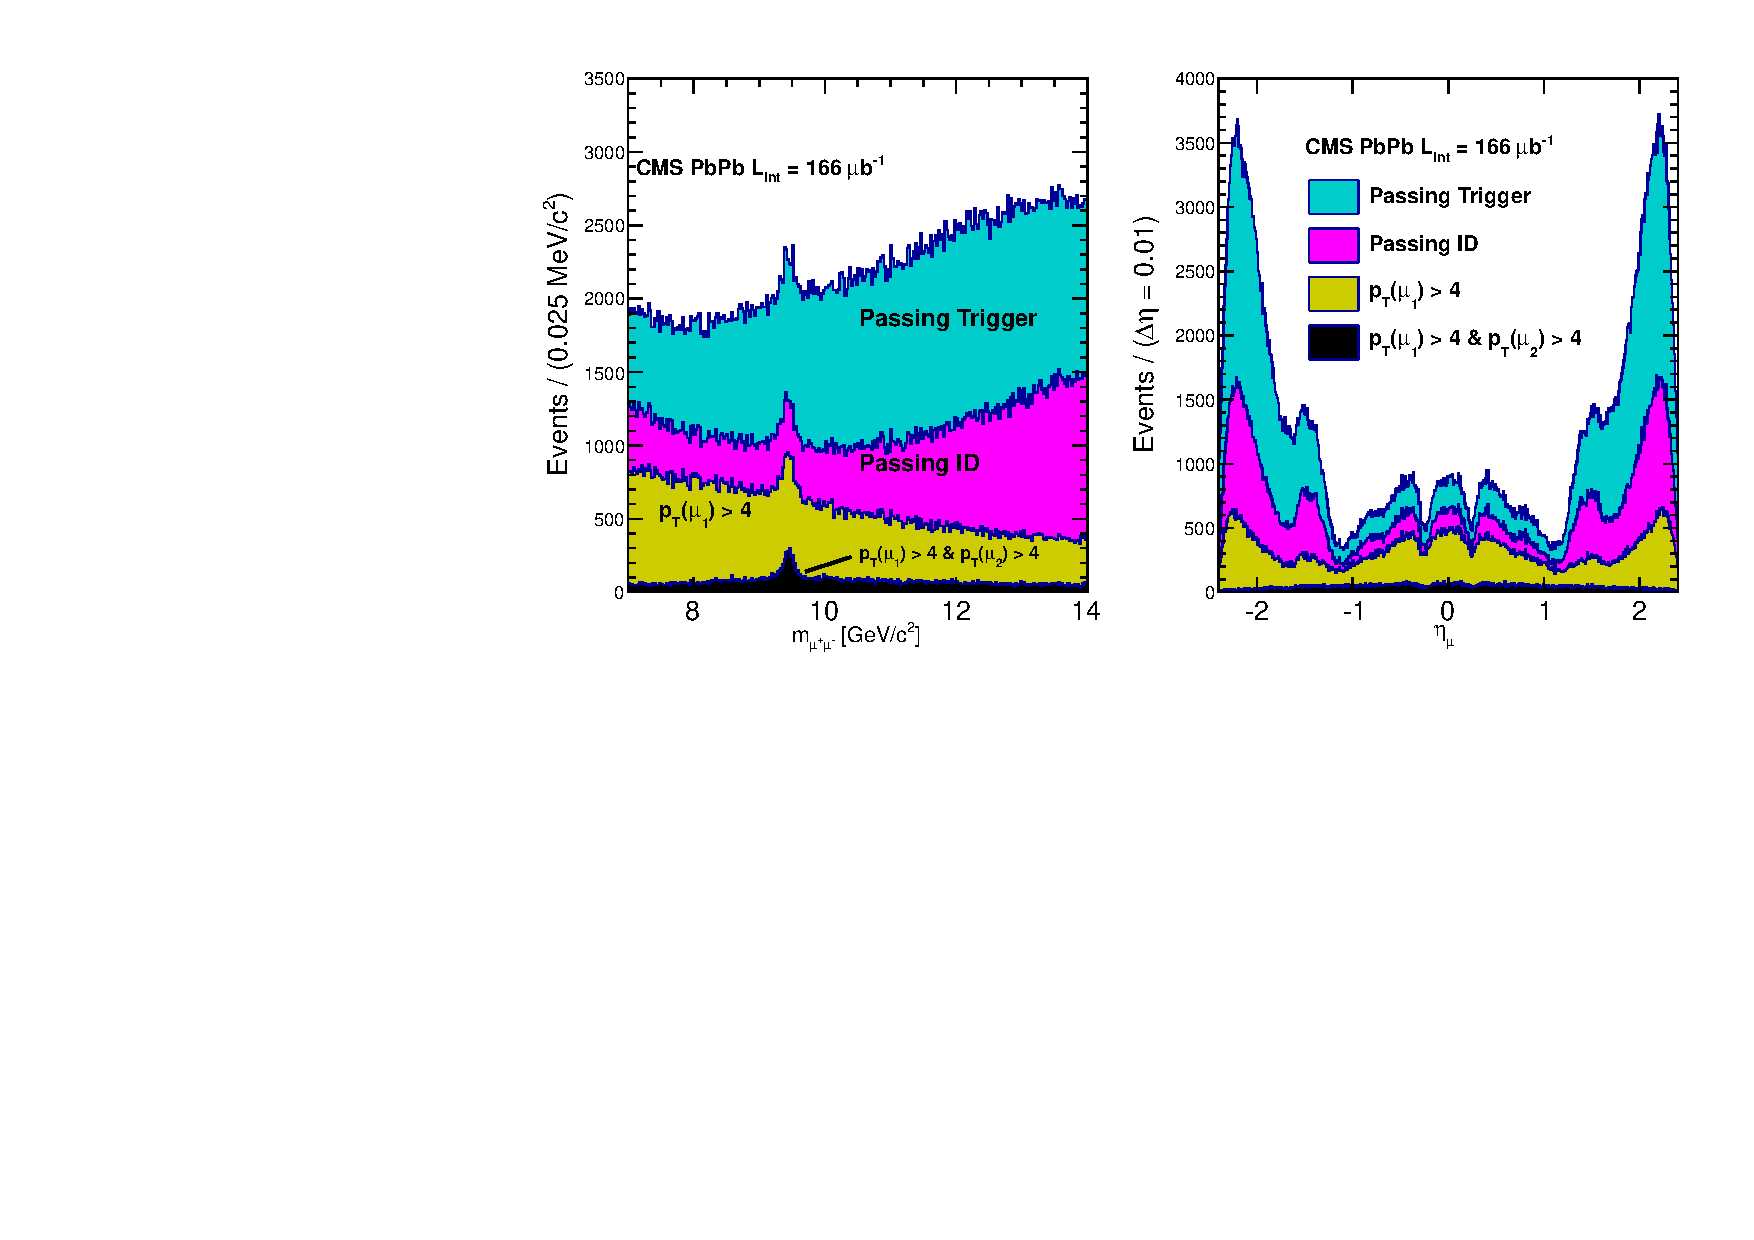
\includegraphics[width=\textwidth]{Chapters/aYield/noCuts_pt4.pdf}
\caption{PbPb data in the \PgU\ mass range, following three
  successive cuts. Samples in decreasing size are (cyan) the events
  firing the analysis trigger, (magenta) subsequent events passing the analysis
  ID cuts, (gold) subsequent events with one muon  of \pt above 4~\GeVc, (black) events with both muons above 4~\GeVc. Left: dimuon invariant mass, right: muon pseudorapidity. Integrals of events are tabulated in Table~\ref{tab:totalNevts}.}
\label{fig:HIdata2011}
\end{center}
\end{figure}

\begin{table}[h]
  \begin{center}
    \begin{tabular}{|c|c|}
\hline
     Type of cut & Number of events, $m_{\mu\mu} \in [7,14] \; \unitMass$ \\
      \hline
      \hline
      Passing \verb?HLT_HIL1DoubleMu0_HighQ?& 620640\\
      Passing muon ID cuts& 320393 \\ 
      $\pt(\mu_{1}) > 4 \; \GeVc $ & 161510\\  
      $\pt(\mu_{1})$ and $\pt(\mu_{2}) > 4 \; \GeVc$  & 21692\\
      \hline
      % pt = 3.5, 4 &Gain in  m$_{\mu\mu}\in $ [7,9.2[ &  Gain in MC
      % Signal & Gain in m$_{\mu\mu}\in $ [9.7,14] \\
      % \hline
      % \hline
      %  $|y| <$  0.8       &79.9\%& 17.9\%& 81.3\% \\
      % 0.8   $< |y| <$  1.6 &96.1\%& 21.5\%& 68.1\% \\ 
      % 1.6   $< |y| <$  2.4 &79.9\%& 17.9\%& 81.3\% \\ 
      % \hline      
      % pt = 3.5, 4.5 &Gain in  m$_{\mu\mu}\in $ [7,9.2[ &  Gain in MC Signal &Gain in m$_{\mu\mu}\in $ [9.7,14] \\
      % \hline
      % \hline
      %  $|y| <$  0.8       &40.5\%& 15.3\%& 45.4\% \\ 
      % 0.8   $< |y| <$  1.6 &47.2\%& 18.5\%& 43.4\% \\
      % 1.6   $< |y| <$  2.4 &40.5\%& 15.3\%& 45.4\% \\
      % \hline
      % pt = 3, 4 &Gain in m$_{\mu\mu}\in $ [7,9.2[ &  Gain in MC Signal
      % &Gain in  m$_{\mu\mu}\in $ [9.7,14] \\
      % \hline
      % \hline
      %  $|y| <$  0.8       &109\%& 22.4\%& 166\%\\ 
      % 0.8   $< |y| <$  1.6 &206\%& 32.7\%& 125\%\\
      % 1.6   $< |y| <$  2.4 &109\%& 22.4\% & 166\%\\
    \end{tabular}
  \end{center}
  \caption{Total number of dimuon events in the \PgU\ mass range
    [7,14] \; \unitMass, after applying subsequent cuts (trigger, ID, kinematics).}
\label{tab:totalNevts}
\end{table}

% One can first notice on Figure~\ref{fig:HIdata2011} the large cleaning
% effect of the muon quality cuts, tuned on pp data and used previously in most CMS analyses using
% dileptons in heavy ion physics (\cite{torsten,12014,HIN-11-007,11-011}
% are examples). Most of the events cleaned out after applying the
% quality cuts contained for example one or two muons with a poor
% standalone muon segment in the muon stations. 
When removing low quality muons from the dataset, the dimuon background is
halved, and the \PgUa\ peak also appears clearer, its height apparently unaltered. In turn, cutting on the
kinematics of the recorded muons (gold and black histograms) plays a role in removing
most of the background in the mass plot and maintain most of the
\PgUa\ peak. Because of the large y-axis scale of the left hand side plot in
Figure~\ref{fig:HIdata2011} it is hard to tell whether excited \PgUb\
can be seen at all, however a closer look in the following Sections
will provide more information on this subject.


On the right hand side of Figure~\ref{fig:HIdata2011}, several
observations can be made. First, at $\eta \sim \pm 0.3$, dead areas
between Wheel 0 and Wheel 1 of the steel yoke are responsible for the
loss of events in that region. A similar feature appears with $\eta
\sim \pm 1.1$, along with the change of material distribution from
barrel to endcap. In the forward region, muons need a smaller \pt\ to
reach the muon stations: this results in a very large background of
soft muon events, which has been reduced by more
than half when applying the muon ID cuts. This could be the sign of
pion and kaon decays, as seen in
Section~\ref{sec:muonID}, the muons with a large distance to the
primary vertex being cleaned away in our analysis. 


In previous analyses of \PgU\ in CMS, an offline $\pt > 4 \; \GeVc$ cut
was applied to both muons. After applying this cut in the present data, the remaining events
are presumably originating from a hard process, such as
quarkonium production, heavy flavour decays and Drell-Yan. We see from
the comparison between gold and black histograms of
Figure~\ref{fig:HIdata2011} that some of the
\PgU\ signal is lost in the $\pt > 4 \; \GeVc$ cut, while a lot of the background has
been cut away. 

\begin{figure}[h]
  \begin{center}
    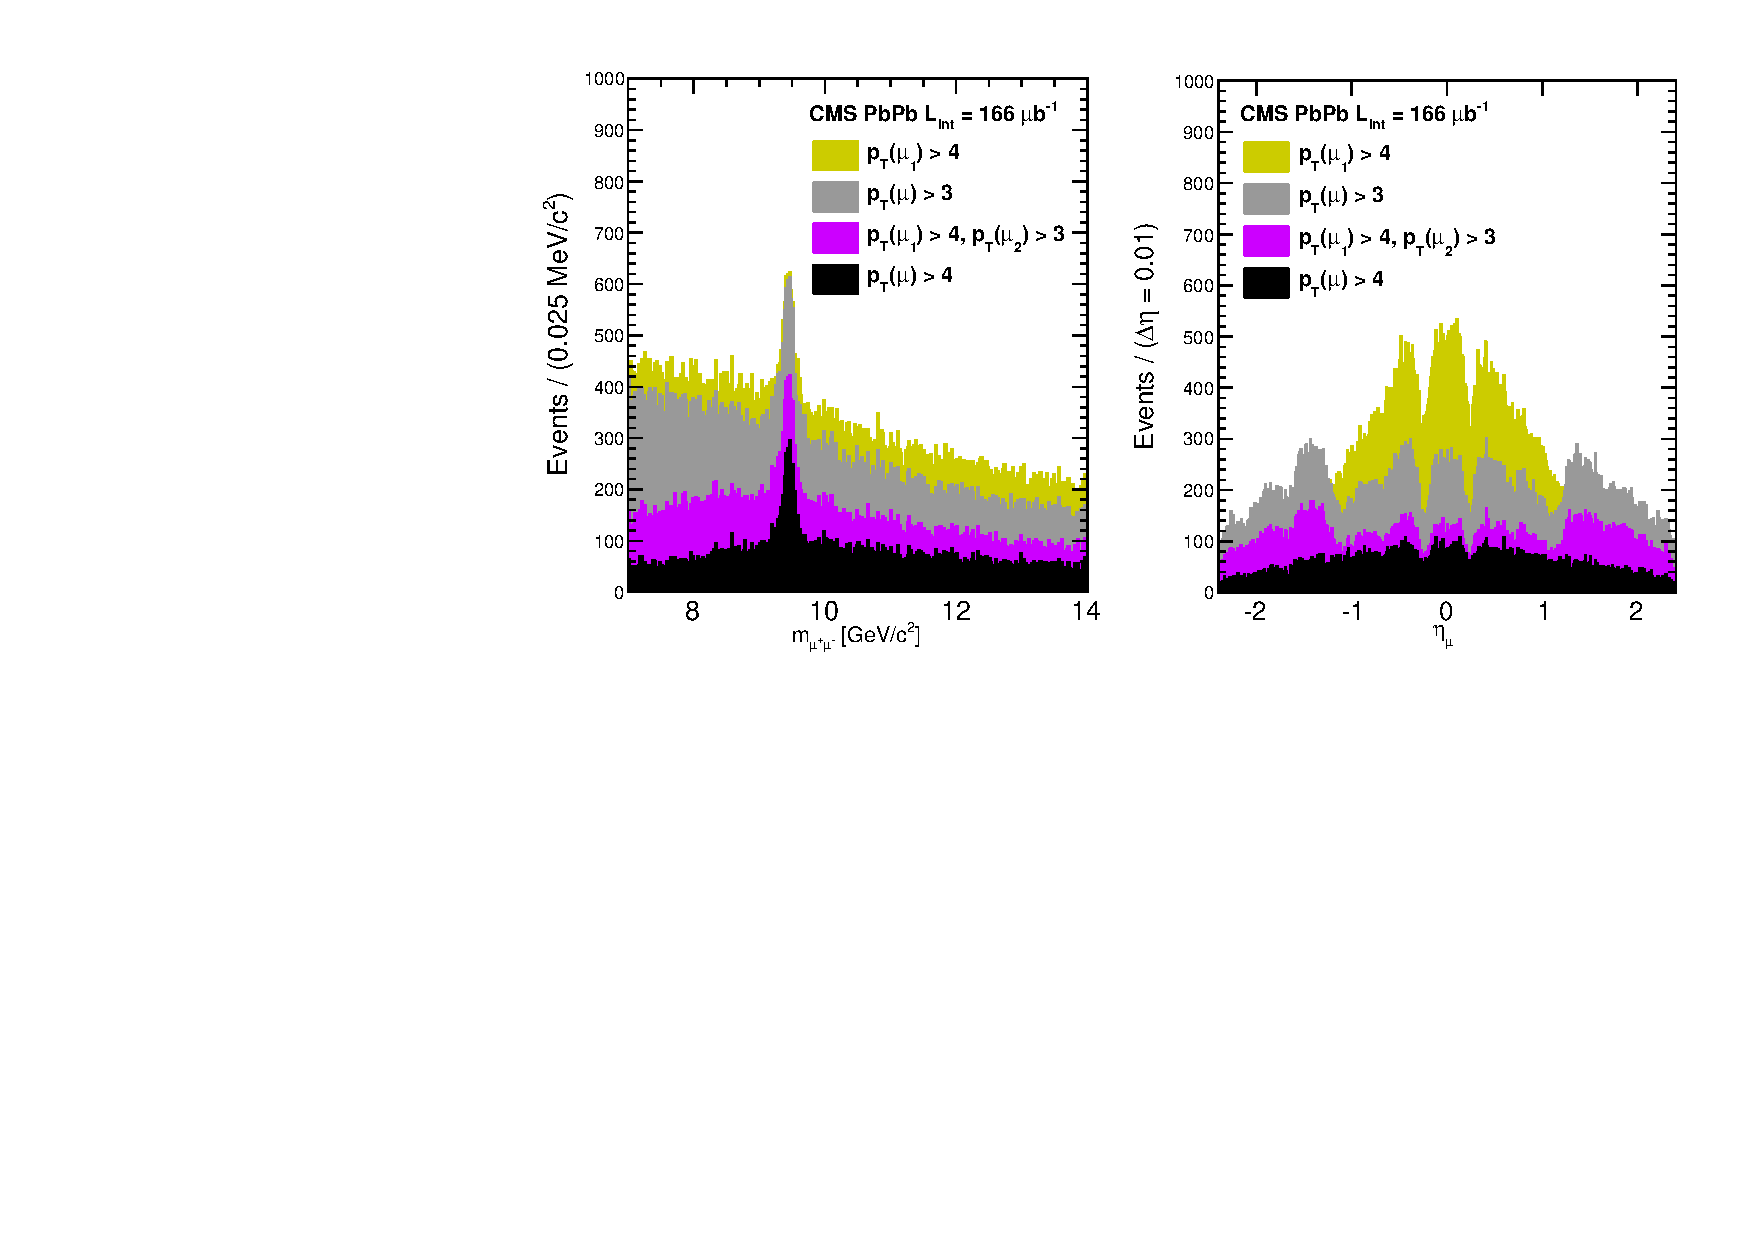
\includegraphics[width=\textwidth]{Chapters/aYield/variouscuts.pdf}
    \caption{PbPb data in the \PgU\ mass range, for various cuts on the
      single muon transverse momentum. Gold and black histograms are
      equivalent to Figure~\ref{fig:HIdata2011}. Gray corresponds to a
      $\pt > 3$ cut looser than gold, however applied on both muons. Violet corresponds
      to an asymmetric cut where one muon has a $\pt > 3$ cut, while the
      second has a $\pt > 4$ cut (independently of the charge).}
    \label{fig:tryptcuts}
  \end{center}
\end{figure}

Pushing further the comparison between the gold histogram
($\pt(\mu_{1}) > 4 \; \GeVc$) and the black histogram ($\pt(\mu_{1,2}) > 4 \; \GeVc$) of
Figure~\ref{fig:HIdata2011}, I have tried several sets of \pt\ cuts
to get a clear insight of what was the kinematics of the events in
the PbPb sample. The goal was to get the best signal at the edge the
rapidity distribution, as well as at low \pt. Figure~\ref{fig:tryptcuts} shows what can be done when tuning the \pt
cuts of the two muons, either in conjunction or separately: When the
\pt\ threshold is the only difference between two cuts (as in grey
\vs. black histograms) the number of events passing cuts decreases quite
constantly with pseudorapidity. The amount of decrease depends on the \pt\ difference between the
two cuts. Tightening the cut further would only reduce the
yield. Next, by releasing the cut applied to only one of the muons (as
is black \vs. pink histograms), the number of events increases more at
large pseudorapitities than in the barrel region. This is a
\textit{flattening} of the accepted number of events as a function of
pseudorapidity. 
\vspace{0.5em}
 \begin{center}
\fbox{
  \parbox{0.9\textwidth}
  {\textsf {Up to now, we have seen that the excited states are
      suppressed in heavy ions, and a mapping of the kinematics of the
      suppression in the whole \PgU\ sector is crucial. The questions to be answered in this analysis are:
      \begin{itemize}
      \item[-] Does the suppression of individual \PgU\ states appear to
        depend on the kinematics of the resonance?
      \item[-] Is there \PgUa\ suppression in heavy ion collisions, or is it only 
         excited state feeddowns suppression that we see?
      \item[-] Is the \PgUc\ measurable at all?
      \end{itemize} 
      In order to get the most information out of the available PbPb
      data, I have studied how the signal and background behave under
      certain kinematic restrictions on the single muons. % This appeared
      % particularly important because the PbPb dimuon background is
      % very high, and I wanted to secure a significant measurement at
      % forward rapidity and at low \PgU \pt.
      The following Section
      details more about the optimisation of the kinematic cuts,
      looking at signal simulation, as well as $pp$ and PbPb data.}
  }
}
 \end{center}

\section{Statistical optimisation}

Previous analyses on \PgU\ in heavy ions~\cite{HIN-11-007,11-011} performed in the CMS
experiment relied on a $\pt > \;4 \GeVc$ cut on each muon, to discard
much of the large dimuon continuum (called background hereafter). We
have seen in Figures~\ref{fig:HIdata2011} and~\ref{fig:tryptcuts} that
signal and background seem to react differently to muon \pt\ cuts, and
I have tried to benefit from this to optimise the significance of the \PgUa\
(defined as yield over statistical uncertainty) to
secure a satisfactory signal in all bins. This investigation has
started during the first days of 2013, at the time of the $p$-Pb data
taking, when the event display on Figure~\ref{fig:eventmirabilis} was produced from the
first `physics run'% \footnote{A 3D version of this event display has
  % been my desktop wallpaper since then.}
. One can see that for an \PgU\ candidate with
relatively low \pt, the decay appears rather \textit{asymmetric}: one of the
muons takes away a good fraction of the available momentum and
propagates close to the direction of the parent \PgU, while
the other one recoils with a smaller momentum. In the usual $\pt > \; 4 \GeVc$ selection, this event would not have been
kept. 


\begin{figure}[h]
\begin{center}
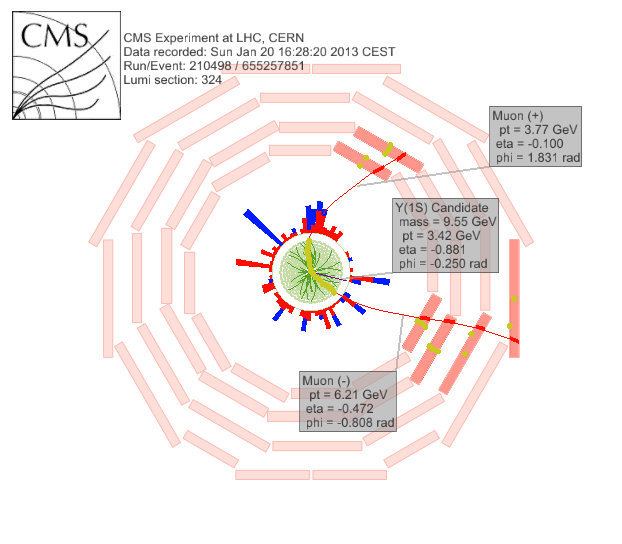
\includegraphics[width=0.8\textwidth]{Chapters/aYield/upsilon_rhophi_detail_white.png}
\caption{Event display of an \PgU\ candidate decaying to two
  muons. View in the transverse plane of the detector (also called
  $r-\phi$ plane). Also shown in green are tracks coming from the rest of the proton-lead
  collision event, and ECAL energy deposits in red and blue.}
\label{fig:eventmirabilis}
\end{center}
\end{figure}

Another account of asymmetric event selection can be found in the 2013
STAR collaboration paper of \PgU\ production in $d$Au collisions~\cite{Adamczyk:2013poh}.

 %the available statistics should allow for a precise estimation of the production rate, in 
\subsection{Simulation based studies}

In the following, the effect of various \pt\ cuts is reported for
simulated signal. One should not forget the high background seen in
PbPb: this would be investigated further.%  Assuming a possible physical
% effect on the overall \PgU\ population (for example, a \pt\ dependent
% suppression), the cuts of interest will thus be tested against data
% based signal as well.

In Figure~\ref{fig:MCtries} left and right, the dimuon mass and muon
$\eta$ distributions are presented for various complementary \pt\ intervals. The
histograms have been stacked as to represent the contribution of each
\pt\ interval separately. We can see that about 80\% of \PgU\ 
have at least one muon below 5 \GeVc, and almost 45\% have at least one muon
below 4 \GeVc. From the dimuon mass plot (Figure~\ref{fig:MCtries}
left), the resolution of the peak do not seem do depend strongly on
the muon momentum. It can also be seen that the high momentum muons tend
to be rare in the forward region and mostly located in the barrel,
while the lower \pt\ intervals are more evenly distributed in
pseudorapidity. These observations should be correlated with the
individual muon reconstruction efficiency, presented for low-\pt\
muons in the two-dimensional histogram of Figure~\ref{fig:simpleacceptance}.

\begin{figure}[h]
\begin{center}
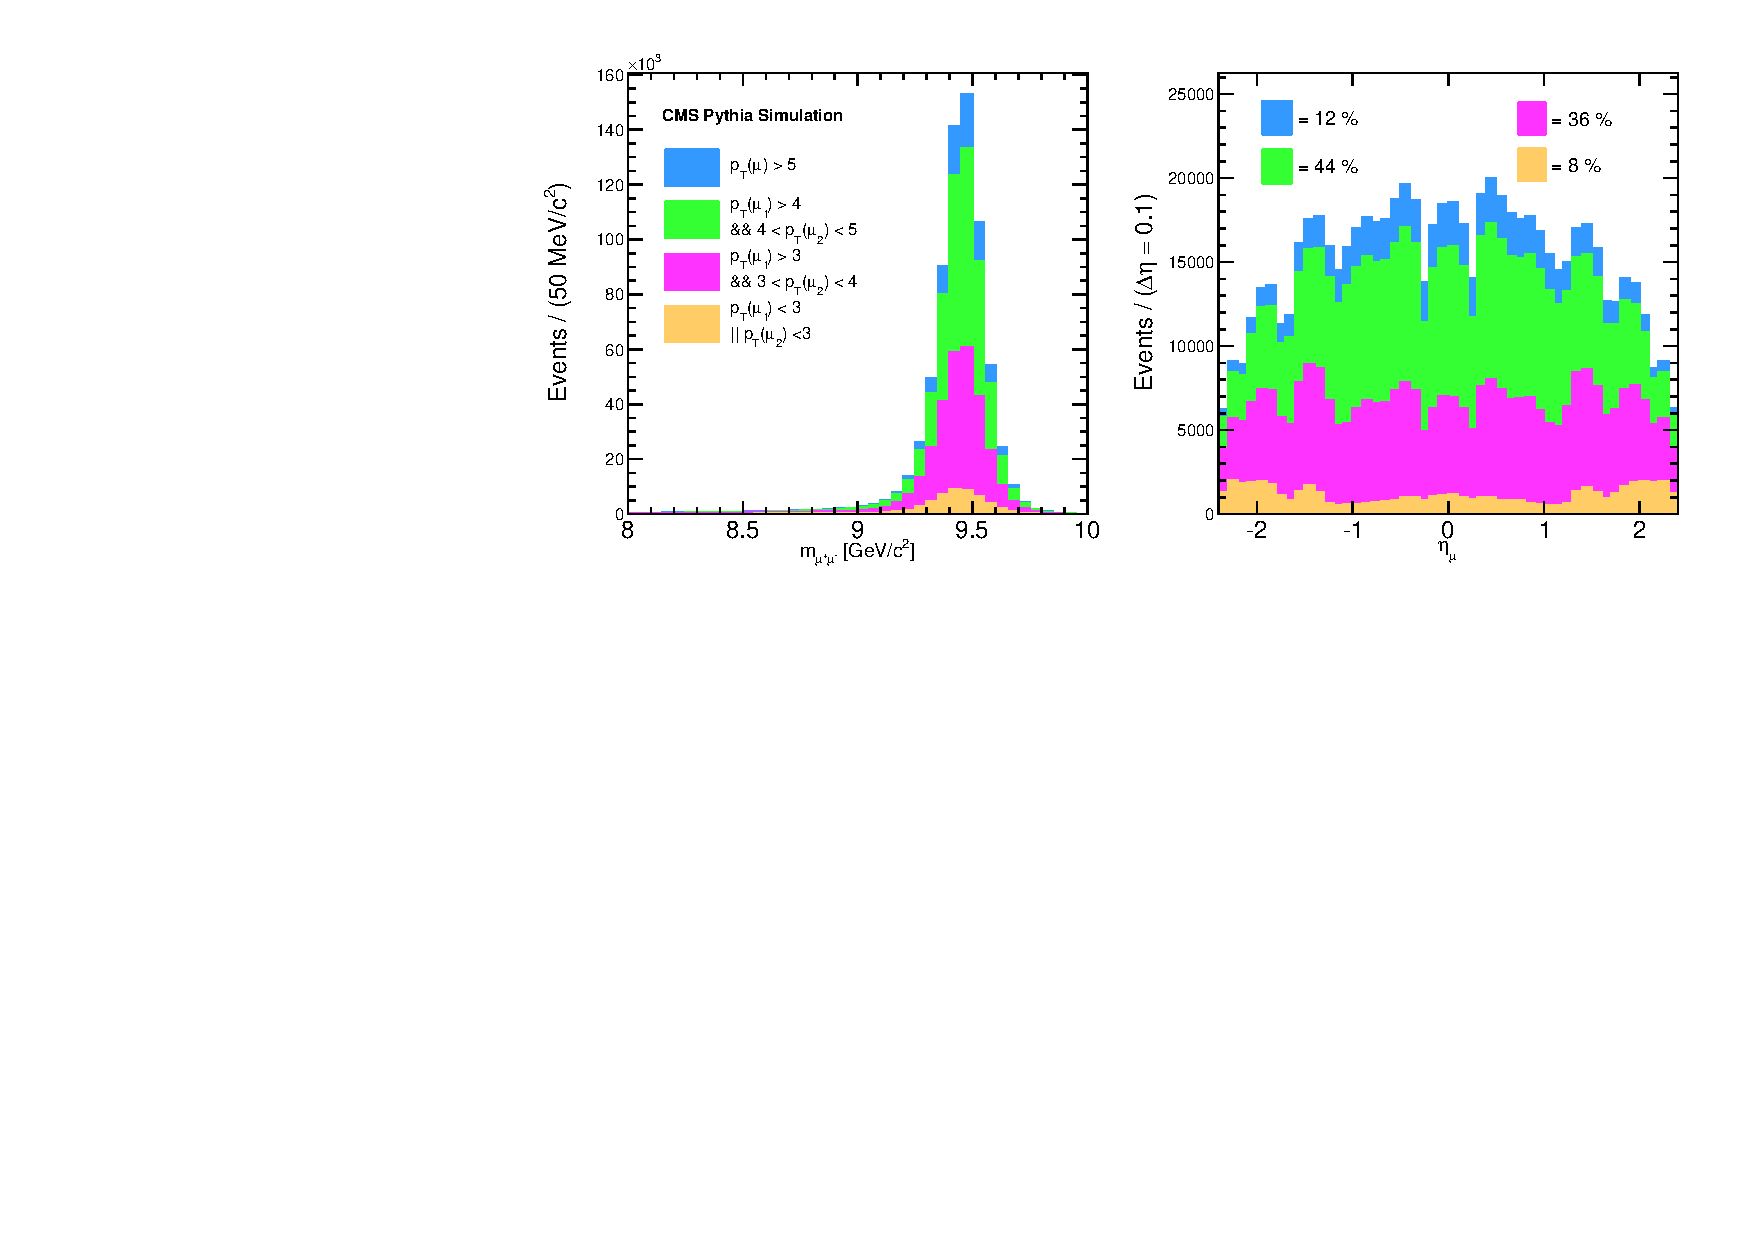
\includegraphics[width=\textwidth]{Chapters/aYield/MCtries.pdf}
\caption{\PgUa\ simulated events reconstructed in CMS, for various cuts on the
      single muon transverse momentum. The dimuon mass spectrum is
      presented on the left, and the pseudorapidity distribution of
      decay muons is displayed on the right. Histograms are stacked because
      of their complementarity. Colours
      correspond to complementary single muon \pt\ ranges.}
\label{fig:MCtries}
\end{center}
\end{figure}

The muons have been generated flat in \pt\ over the whole
pseudorapidity coverage of CMS muon stations. The effect of the
magnetic field is clearly visible; below a certain threshold defining
going as high as \pt\ $\simeq$ 3.2 \GeVc, muons are not reconstructed.
This \textit{edge of the acceptance} is our limit for the muon \pt\ cuts
applied in the analysis, and reduces at higher pseudo-rapidity
because a more significant fraction of the momentum is longitudinal.
% \begin{figure}[h]
% \begin{center}
% 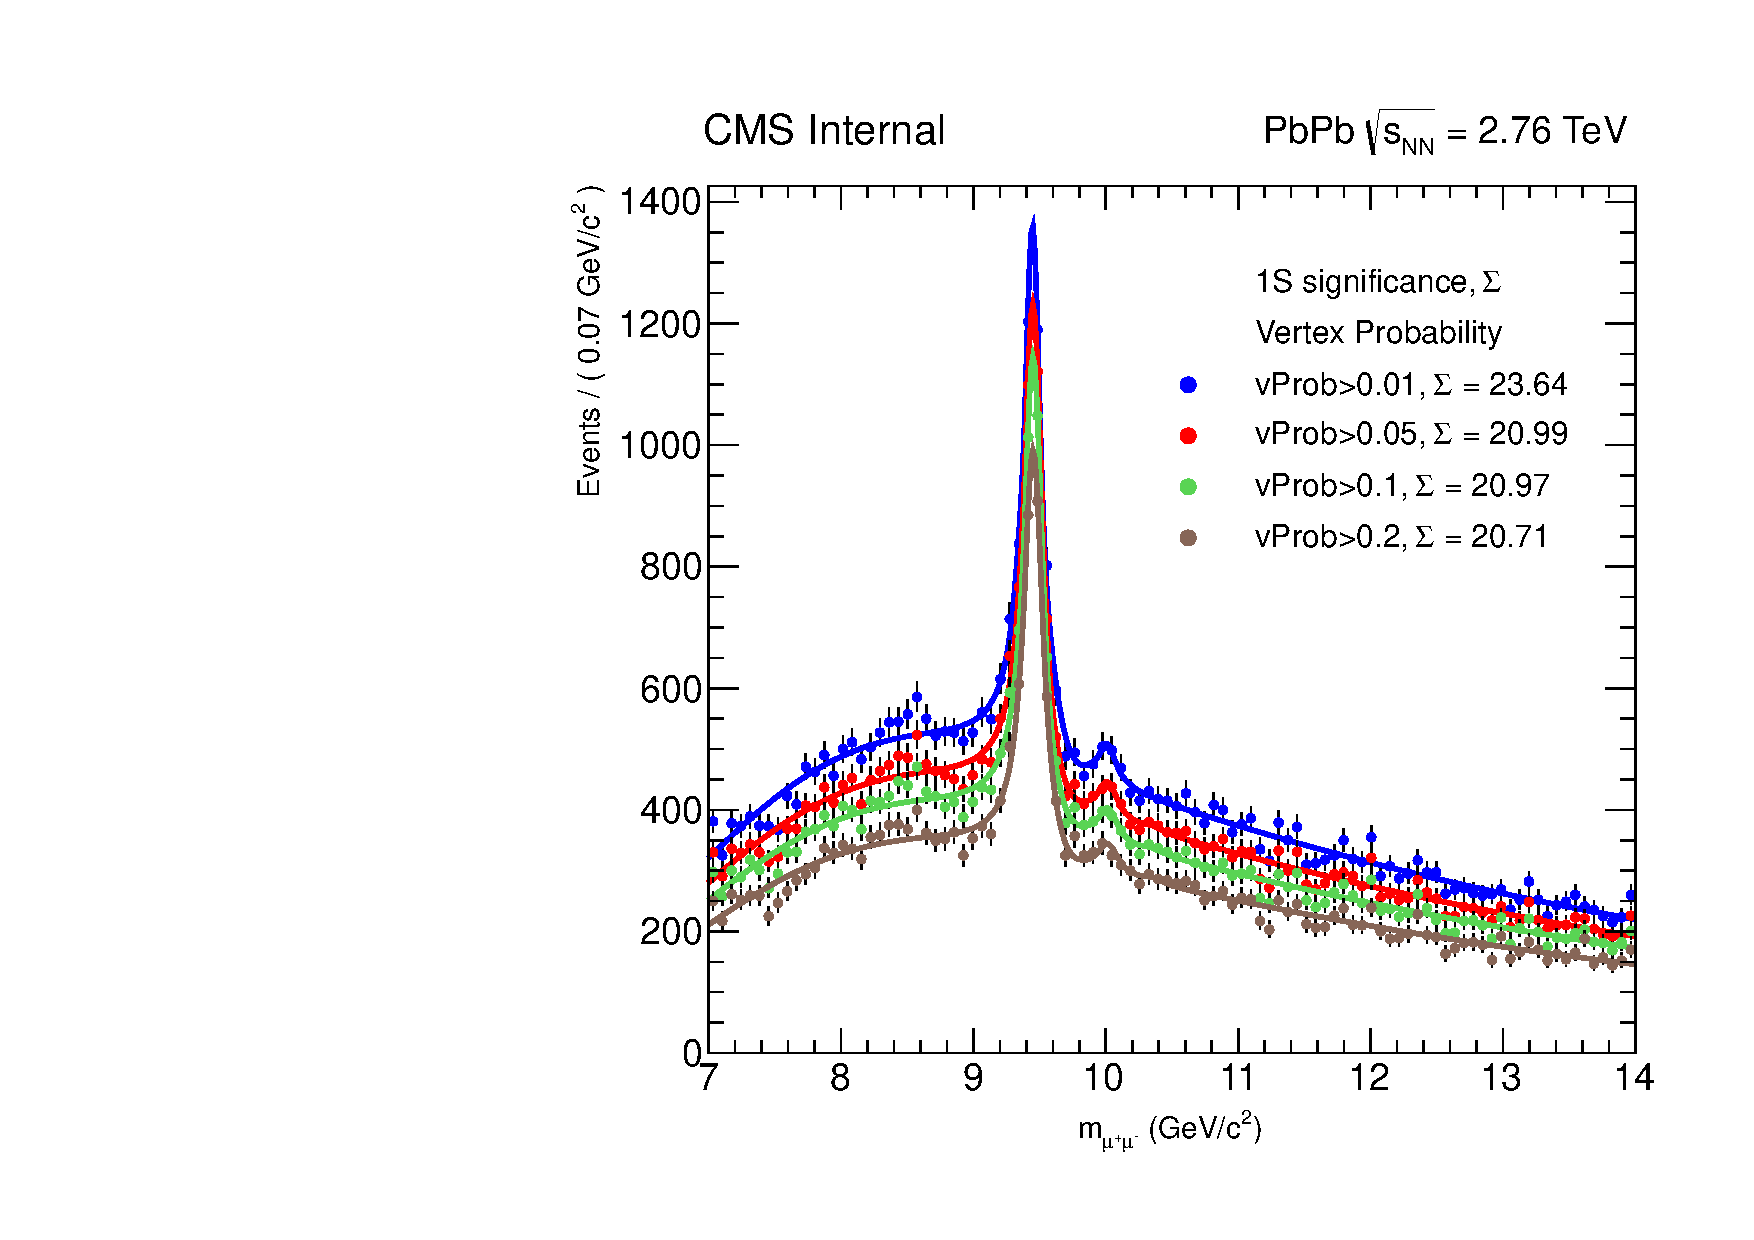
\includegraphics[width=0.2\paperwidth]{Chapters/aYield/vProb_gt0p01.pdf}
% 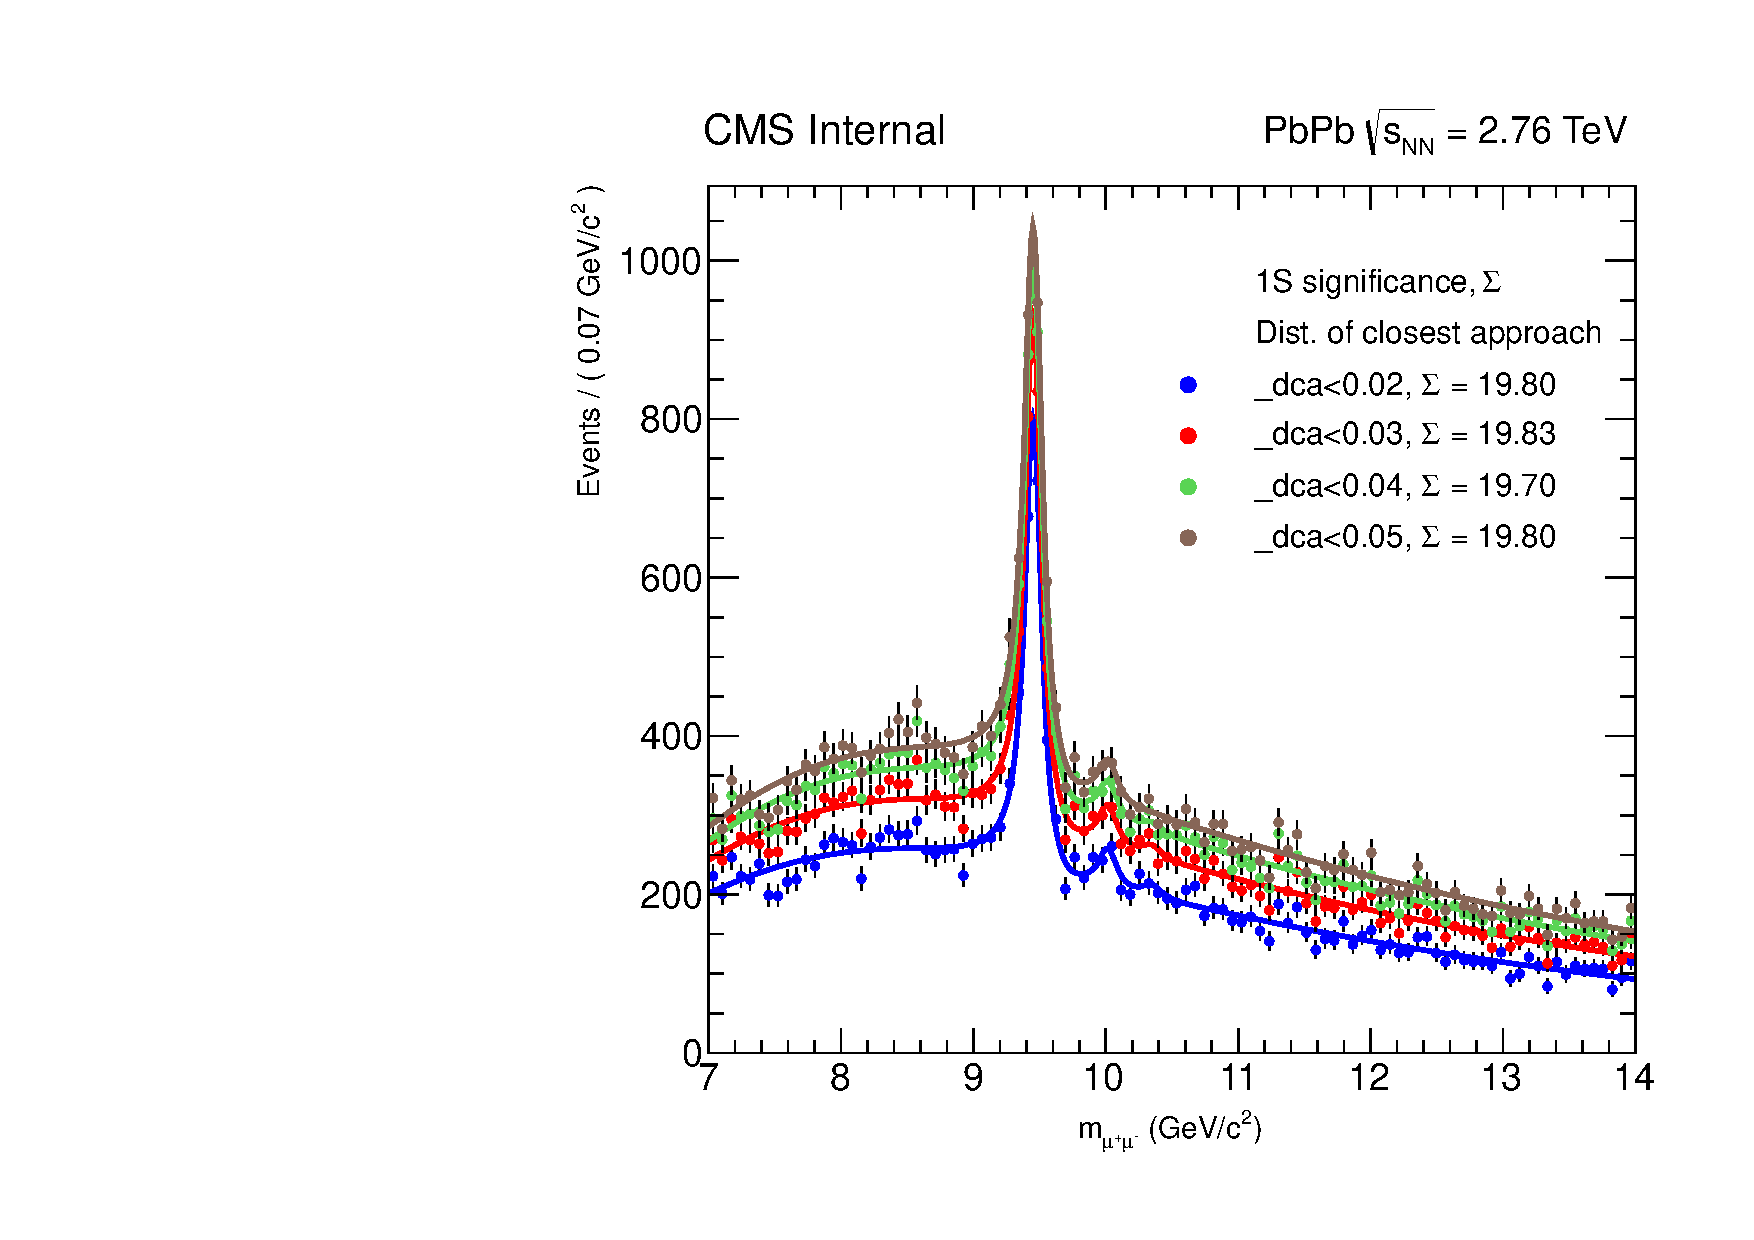
\includegraphics[width=0.2\paperwidth]{Chapters/aYield/_dca_lt0p02.pdf}
% 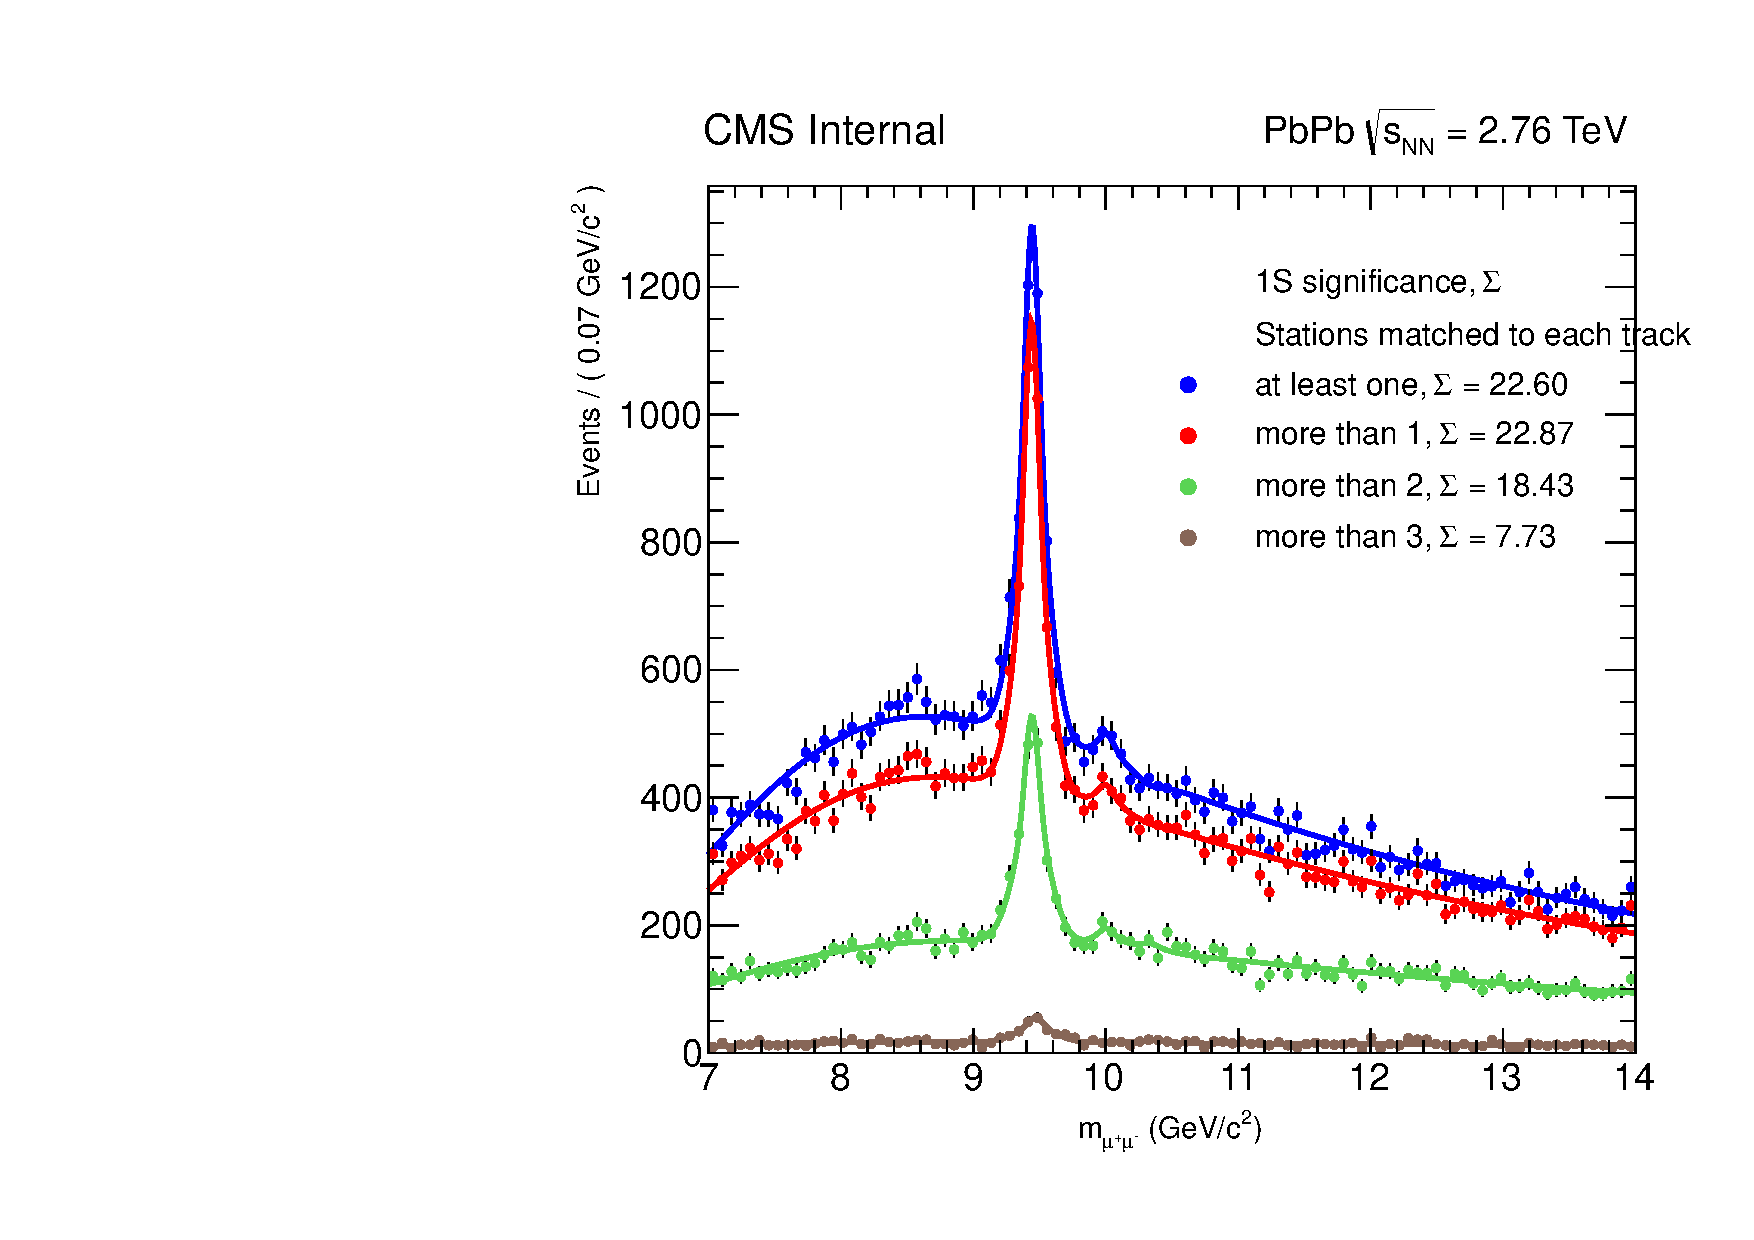
\includegraphics[width=0.2\paperwidth]{Chapters/aYield/_mumi_StationsMatched_gt0_AND__mupl_StationsMatched_gt0.pdf}
% \caption{Fits to PbPb data with several cuts
% on variables \textsc{vProb} (left), \textsc{DCA} (center), and the
% number of matched muon stations to each muon trajectory
% (right). The figures of merit $\Sigma$ quoted in legend
% are equal to the ratio of yield over error for the fitted 1S peak.}
% \label{fig:vProb_dca_MUSTA}
% \end{center}
% \end{figure}
% The solution finally pursued for optimising the figure of merit is \textit{a third one}.

The edge of the acceptance has been previously defined
in~\cite{torsten} as the region where the single muon reconstruction
efficiency is higher than 10\%:

\begin{eqnarray}
\vert\eta^{\mu}\vert < 1.0 & \to & \pt^{\mu} > 3.4 \;\GeVc,  \nonumber  \\
1.0 \leq \vert\eta^{\mu}\vert < 1.6 & \to & \pt^{\mu} > 5.8 - 2.4 \times \vert\eta^{\mu}\vert\; \GeVc,\\
1.6 \leq \vert\eta^{\mu}\vert < 2.4 & \to & \pt^{\mu} > 3.4 - 0.78  \nonumber 
\times \vert\eta^{\mu}\vert\; \GeVc.
\label{eq:acceptanceedge}
\end{eqnarray}

\begin{figure}[h]
\begin{center}
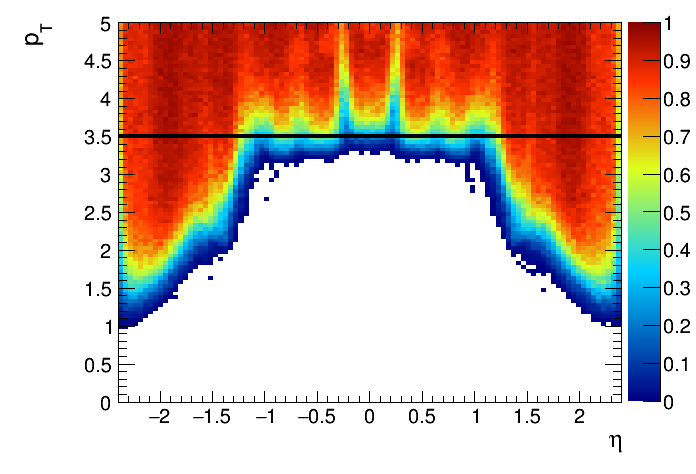
\includegraphics[width=  0.8\textwidth]{Chapters/aYield/smueff.png}
\caption{2D distribution ($p_{T}$, $\eta$) of the muon reconstruction
  efficiency (defined in Section~\ref{chap:aCorrection}), based on a simulated sample of low-momentum muons with
  the PbPb muon reconstruction chain.}
\label{fig:simpleacceptance}
\end{center}
\end{figure}

Considering Figures~\ref{fig:MCtries} and~\ref{fig:simpleacceptance},
it looks like the single muons kinematic cuts could be extended below
\pt = 4 \GeVc. % This
% There, one can see a large blank area in the \textit{central}
% pseudo-rapidity region, The
% acceptance was studied using an official CMS generation campaign of large samples for each
% quarkonium state, using \textsc{Pythia} 6.4. The assumed spectra are not
% flat in \pt\ to accomodate with the real quarkonium production. The
% acceptance is calculated as
% \begin{eqnarray}
% \alpha(\pt,y) & = & \frac{N^{\mu\mu}_{|\eta^\mu|<2.4, {\rm passing}\ \pt^\mu\ {\rm cuts}}(\pt,y,Cent.)}{N^{\mu\mu}_{GEN}(\pt,y,Cent.)} \label{Eq:alpha}
% \label{eq:acc}
% \end{eqnarray}
% where N$^{\mu\mu}_{GEN}$ represents all dimuons generated in the
% (\pt,$y$,Centrality) bin under consideration and
% $N^{\mu\mu}_{|y^\mu|<2.4, {\rm passing}\ \pt\ {\rm cuts}}$
% represents the dimuon pairs for which each muons pass the kinematic $\pt^\mu$ cuts.
% The effect on \PgU\ acceptance of the muon \pt\ = 4 \GeVc\ cut applied
% in the previous analyses
% \cite{PhysRevLett.109.222301}, \cite{Jhep.2012.063} and
% \cite{Jhep.2014.103} is compared to the acceptance when applying no
% \pt\ cuts (hence, looking only at the B field effect) in Figure~\ref{fig:accMapsCutComparison}. Acceptance values are
% displayed in text inside the 2D bins.
% \begin{figure}[h]
% \begin{center}
% 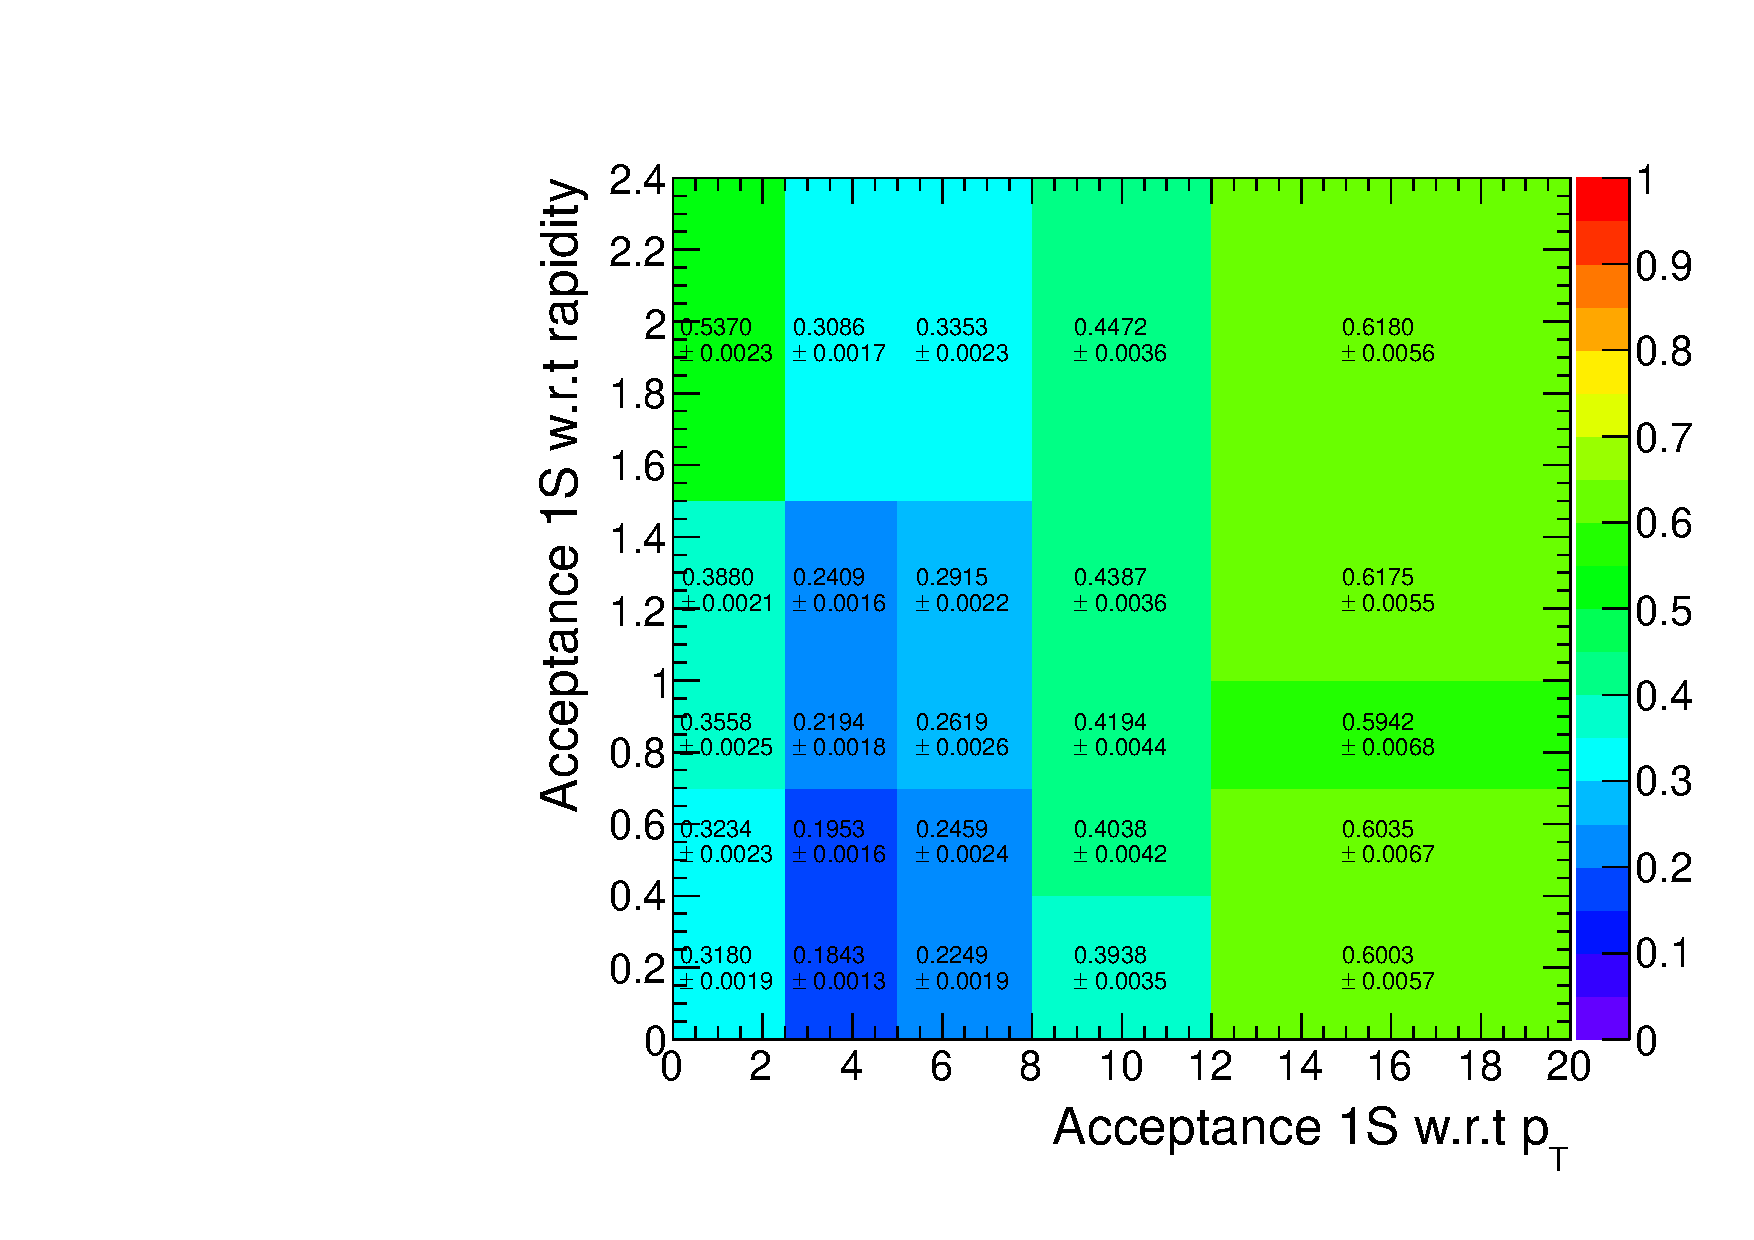
\includegraphics[width=  0.4\textwidth]{Chapters/aYield/acc2D1S_11011.pdf}
% 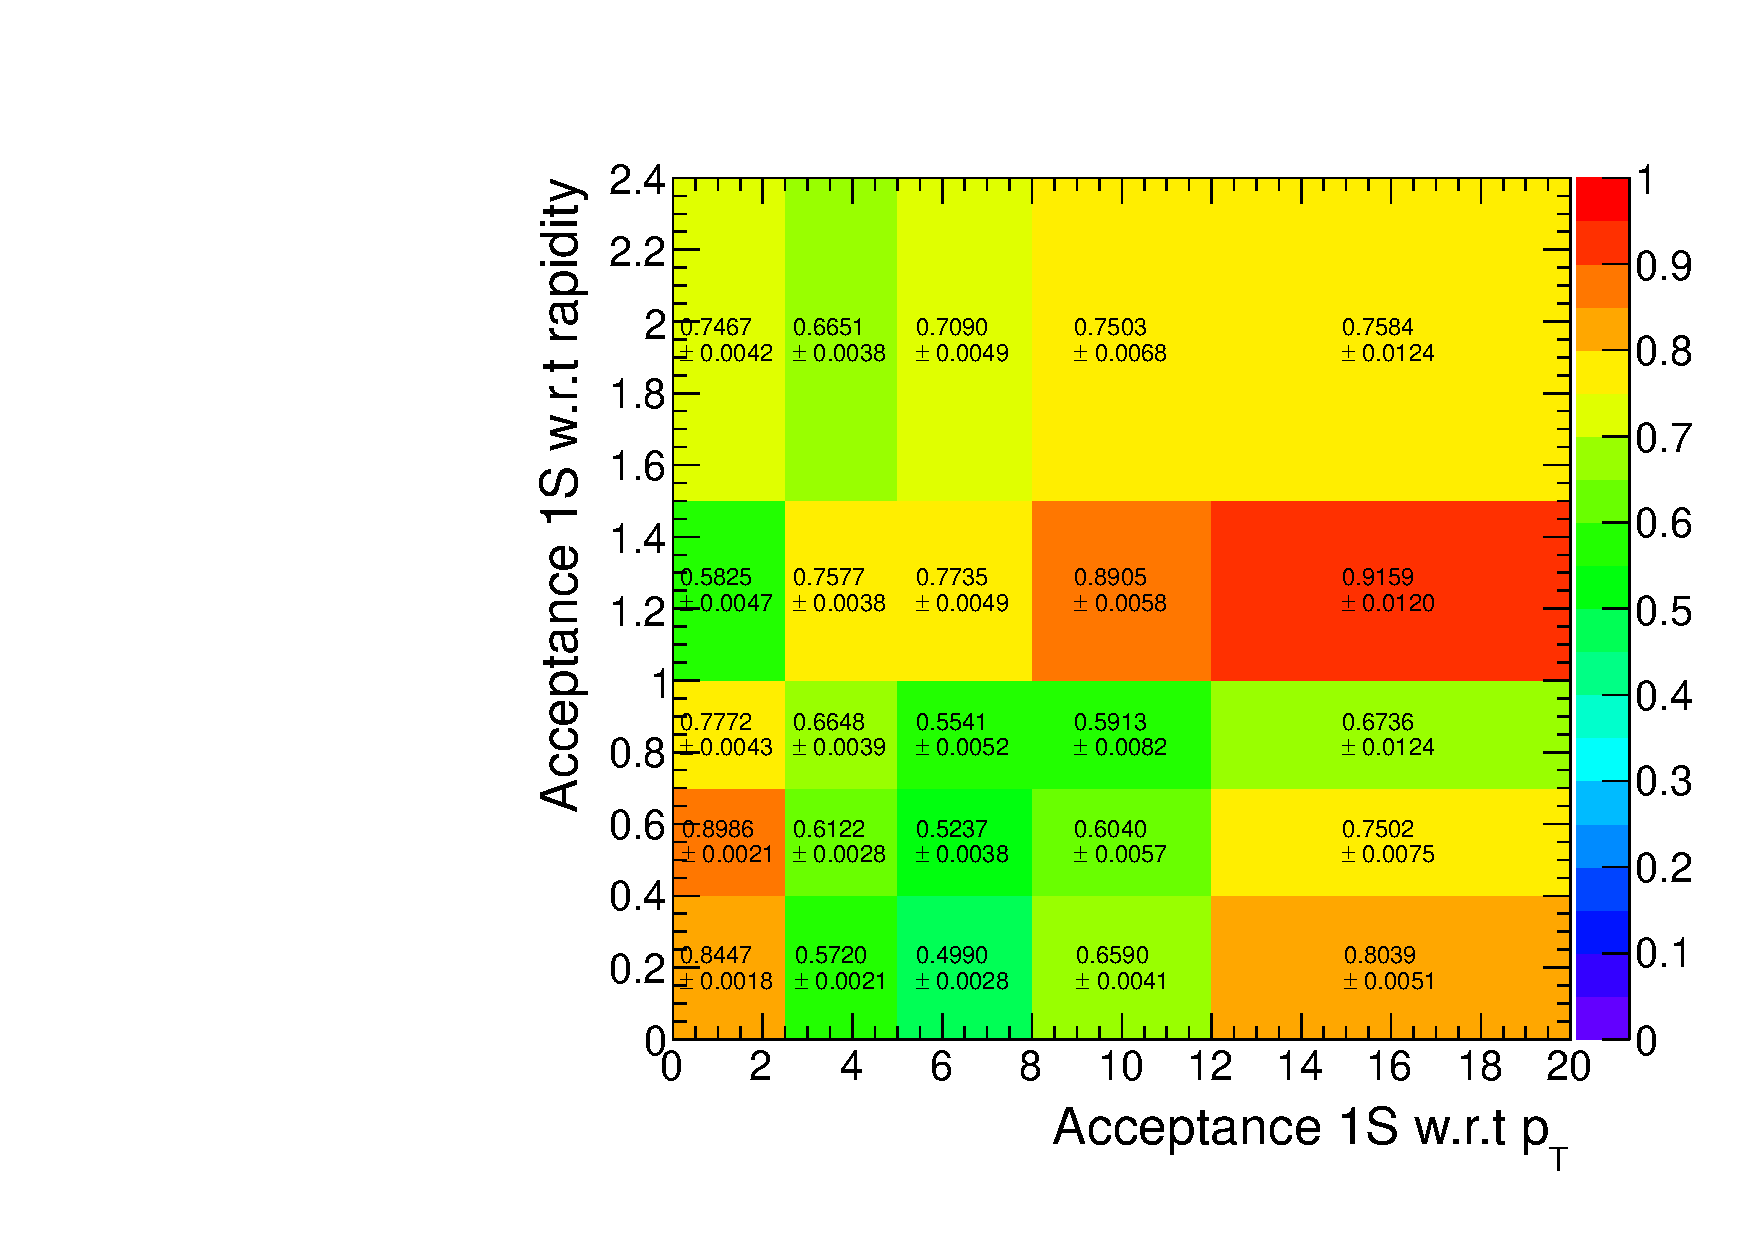
\includegraphics[width=  0.4\textwidth]{Chapters/aYield/acc2D1S_10006.pdf}  
% \caption{Acceptance maps. Single muons cuts applied are, left: 4
%   \GeVc, right: all muons reaching the di-muon reconstruction, see \cite{Jhep.2012.063} for
%   the exact definition ($\eta$-dependent, very loose cut.).}
% \label{fig:accMapsCutComparison}
% \end{center}
% \end{figure}
% From these 2D plots, one can see the $p_{T}^{\PgUa}$-dependent
% variations of the acceptance for each rapidity bin. Also to be noted,
% the mild difference overall of acceptance factors in the left-hand side and
% right-hand side plots. Since this plot was produced with a GEN-level pythia
% sample including no background, it is indicating a significant
% fraction of signal is being discarded by the $p_{T}^{\mu} > 4$~GeV/c cut. 
This has to be tempered by the fact that in data, releasing
such a cut would also enhance the background level.

 The effect of
releasing such cuts on muons in the PbPb sample can be seen on invariant dimuon mass
plots in 
Figure~\ref{fig:massPlotsLooseAndIntermediate}. These histograms are
binned in 3 dimuon rapidity intervals.% , not to be confused
% with muon pseudo-rapidity\footnote{The following relation
%  $y = 1/2(\eta(\mu(1)) +\eta(\mu(2)))$ links the dimuon rapidity to
% the pseudo-rapidity of the two muons.}

To understand the interplay between the background shape increase and
the signal increase, several cuts were tried.
\begin{figure}[h]
\begin{center}
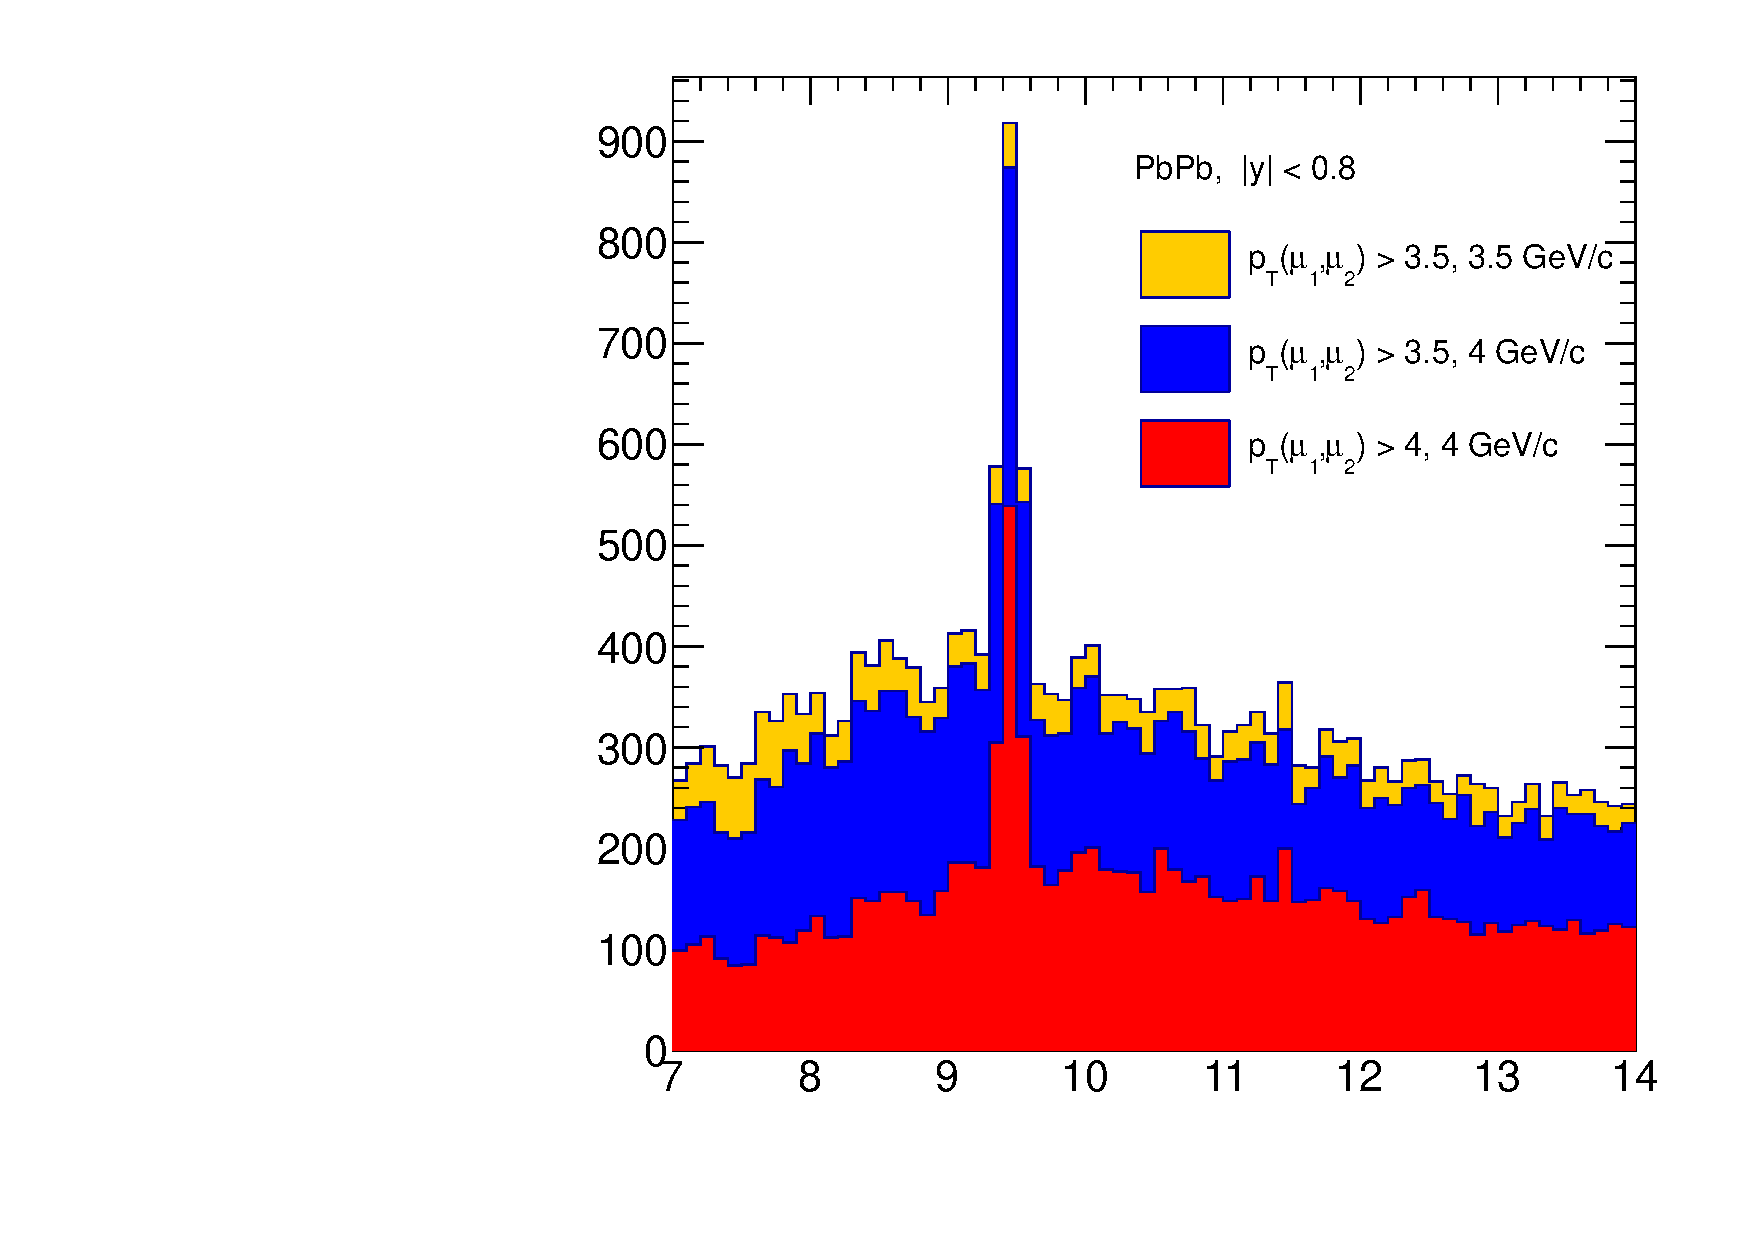
\includegraphics[width=0.3\textwidth]{Chapters/aYield/BarrelMassPlots.pdf}
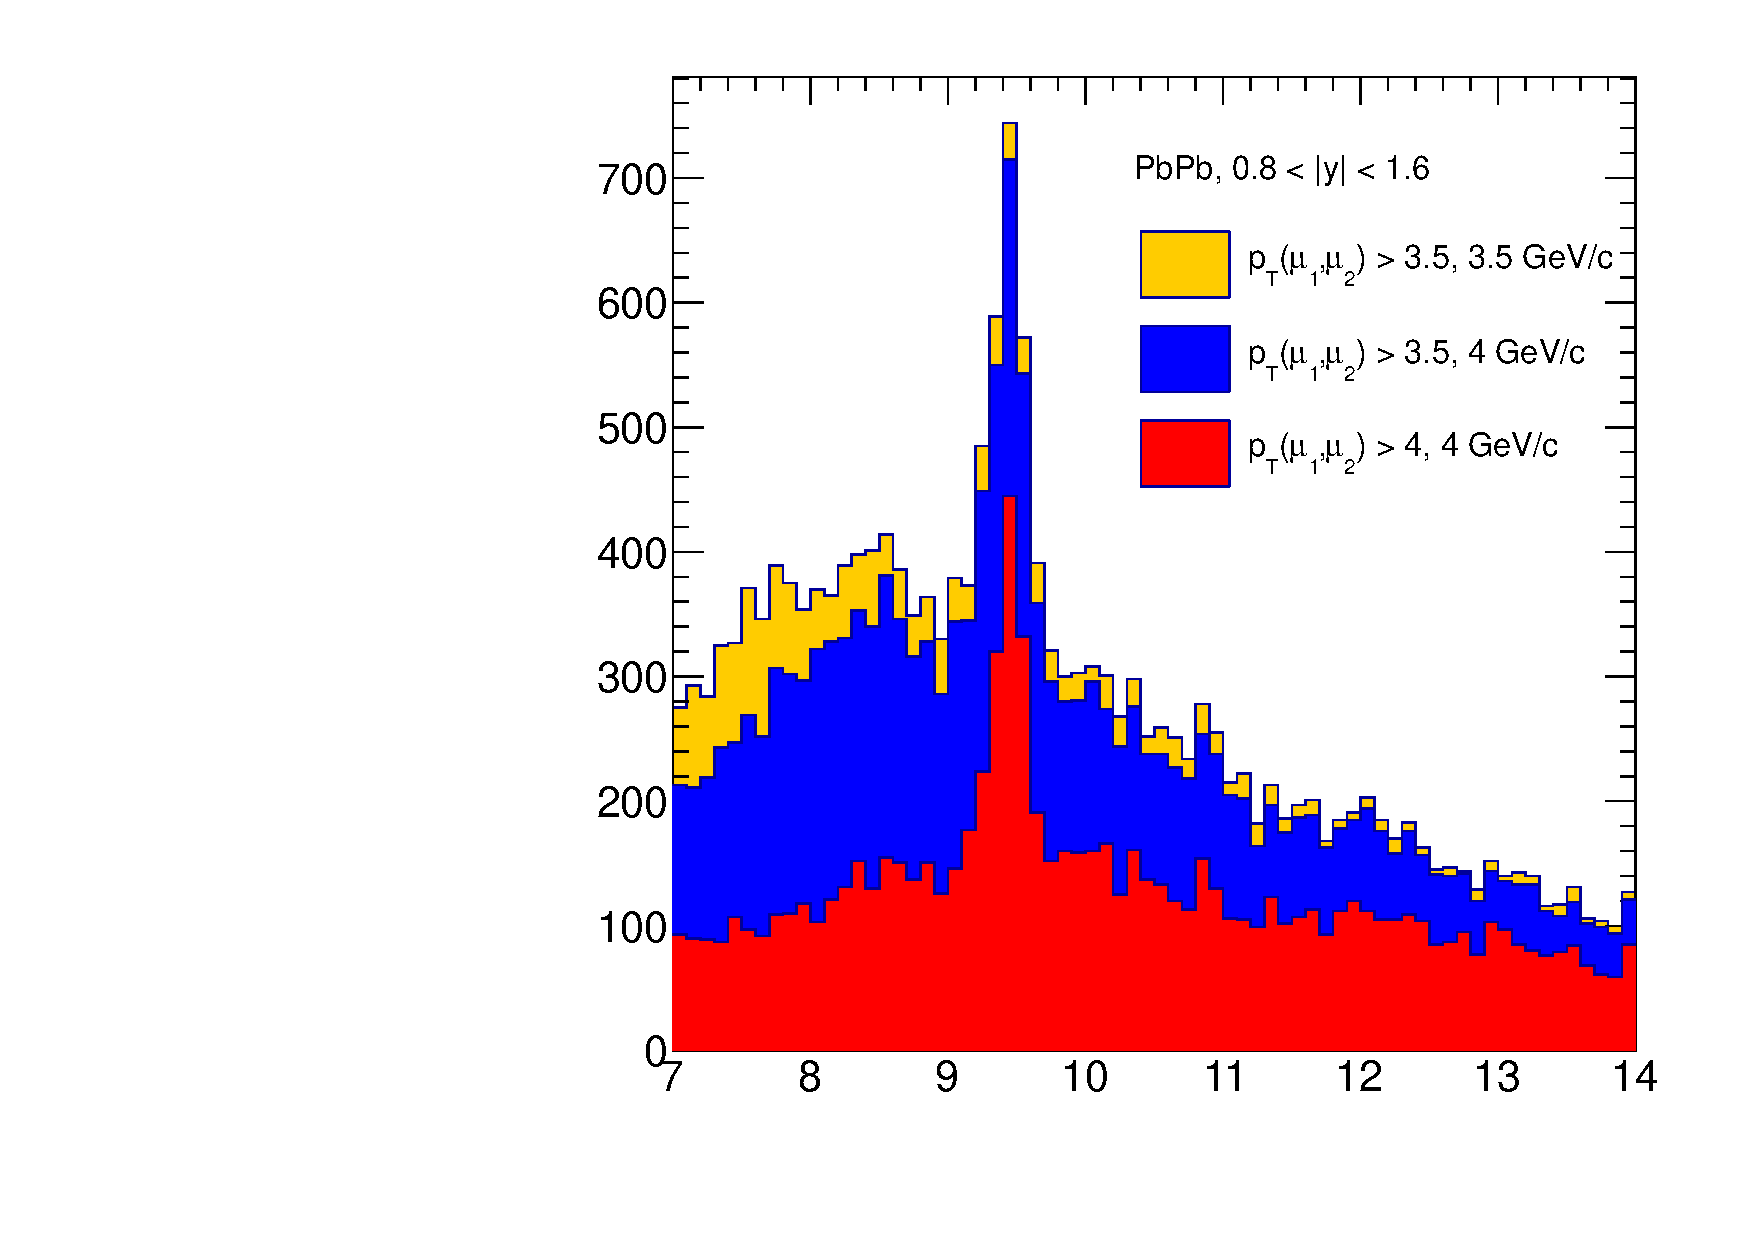
\includegraphics[width=0.3\textwidth]{Chapters/aYield/intermediateRapidityMassPlots.pdf}  
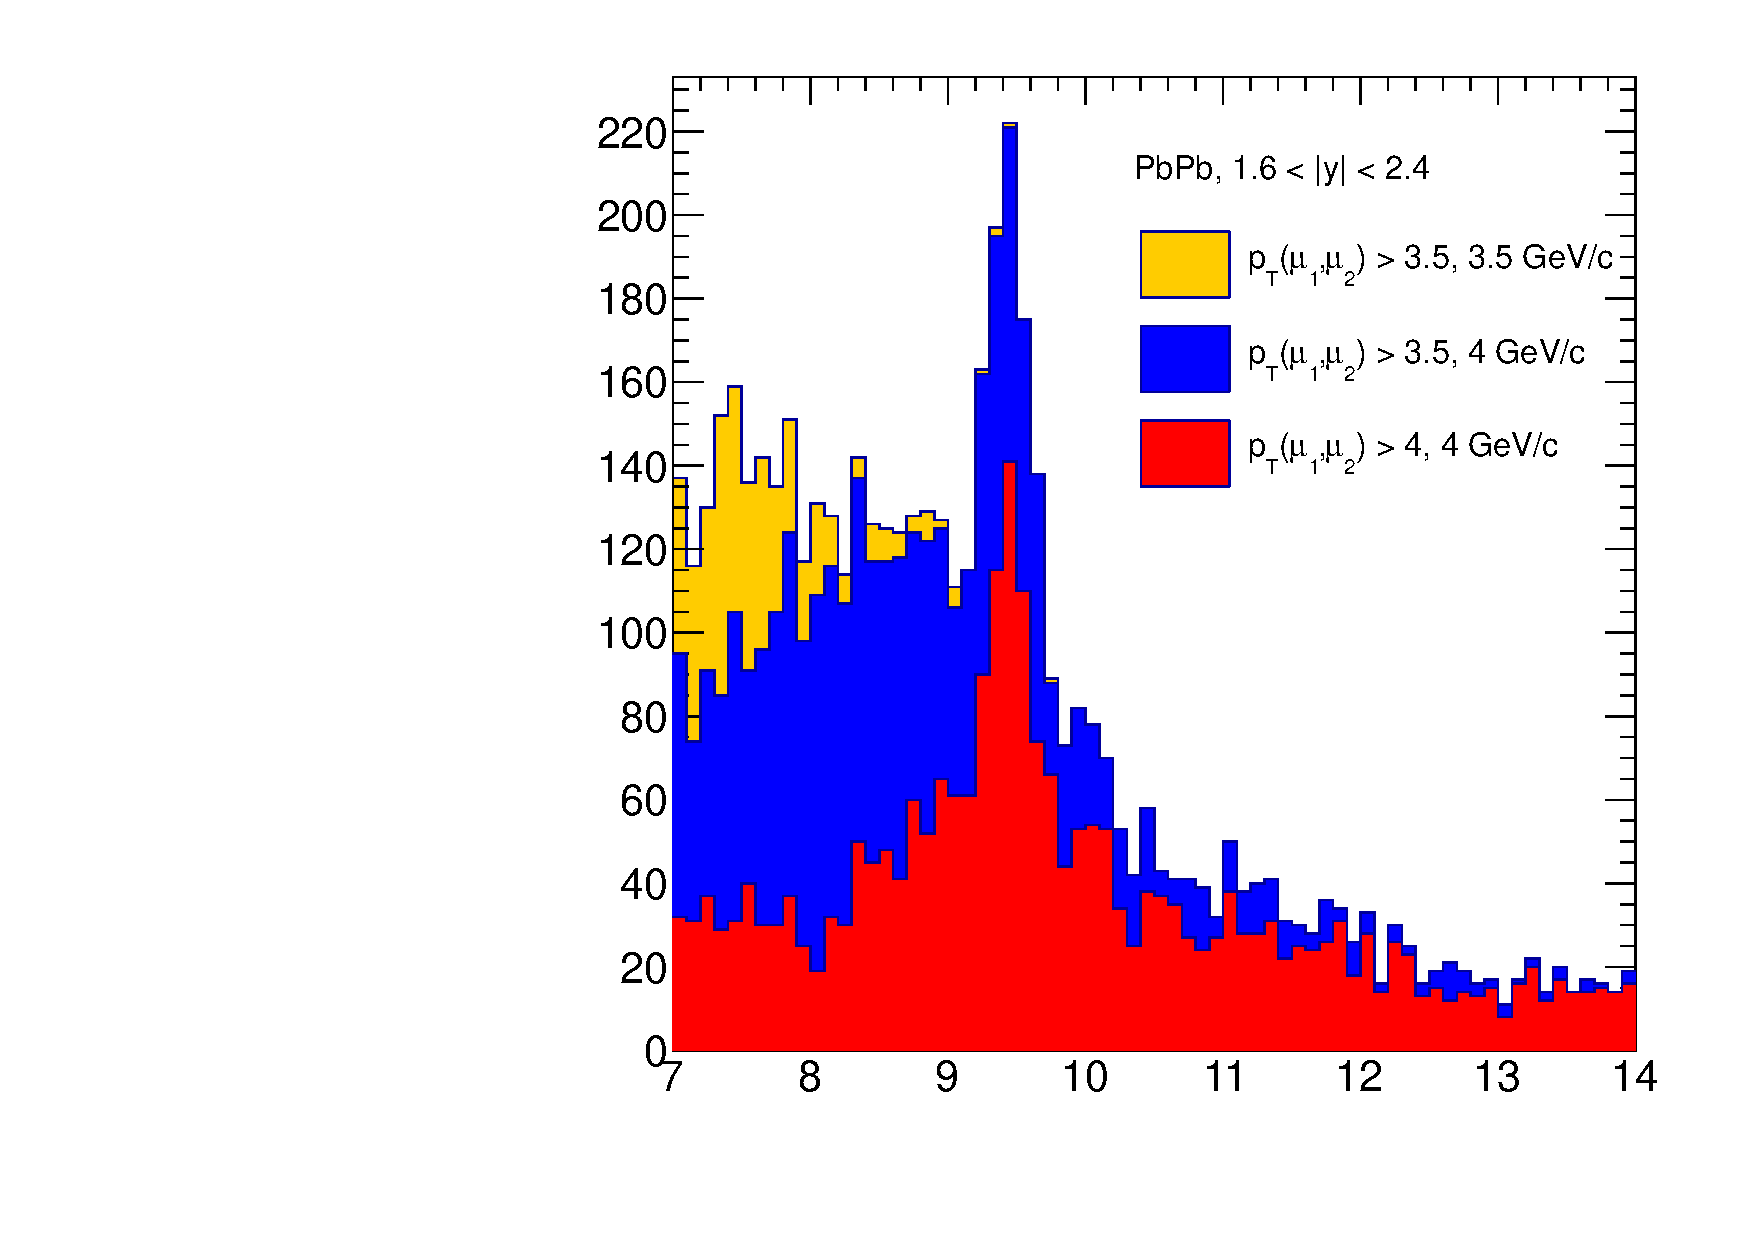
\includegraphics[width=0.3\textwidth]{Chapters/aYield/EndcapMassPlots.pdf}  
\caption{Dimuon invariant mass
  histogram for three different sets of cuts, in three rapidity
  regions: barrel |y|<0.8 (left), intermediate 0.8<|y|<1.6 (center),
  endcap 1.6<|y|<2.4 (right).}
\label{fig:massPlotsLooseAndIntermediate}
\end{center}
\end{figure}
\\
Here follows a list of the cuts applied in Figure~\ref{fig:massPlotsLooseAndIntermediate} and observations related to
them:
\begin{itemize}
\item[-] \textit{Red histogram:}~$\pt(\mu) > 4 \;\GeVc$ is applied to both
  muons. The background seems well behaving and relatively flat, but
  peaking under the \PgUa\ mass peak.
\item[-] \textit{Yellow histogram:}~$\pt(\mu) > 3.5 \;\GeVc$ is applied to both
  muons. The background has largely increased compared to the previous
  case, and its shape clearly changes when moving to forward
  rapidities. The signal peak of \PgUa\ has also increased.
\item[-] \textit{Blue histogram:}~$\pt(\mu_{1}) > 3.5 \;\GeVc$ and
  $\pt(\mu_{2}) > 4 \GeVc$ is applied. This asymmetric cut seems to
  reduce background of a certain amount, while leaving the signal
  untouched, compared to the blue histogram case. 
\end{itemize}


To better illustrate the motivations for an asymmetric muon \pt\ cut to
isolate signal from background, let us look at the 2D distribution of
Figure~\ref{fig:twoMuonsPt}, where the \pt\ of each muon is reported on
x- and y- axes, for PbPb simulation and data.  The signal \PgU\ produces two muons with
anti-correlated \pt, which is understandable by kinematics of the
decay. When the resonance is produced with a given \pt, the decay in
the rest frame of the experiment is asymmetric, one muon taking away
more momentum than the second. On the right hand side of
Figure~\ref{fig:twoMuonsPt}, one can see
the bulk of the muon multiplicity produced in PbPb collisions is
located at low \pt\ values, necessarily in the forward region since
such low momentum values can only be reached in the endcaps.

\begin{figure}[h]
\begin{center}
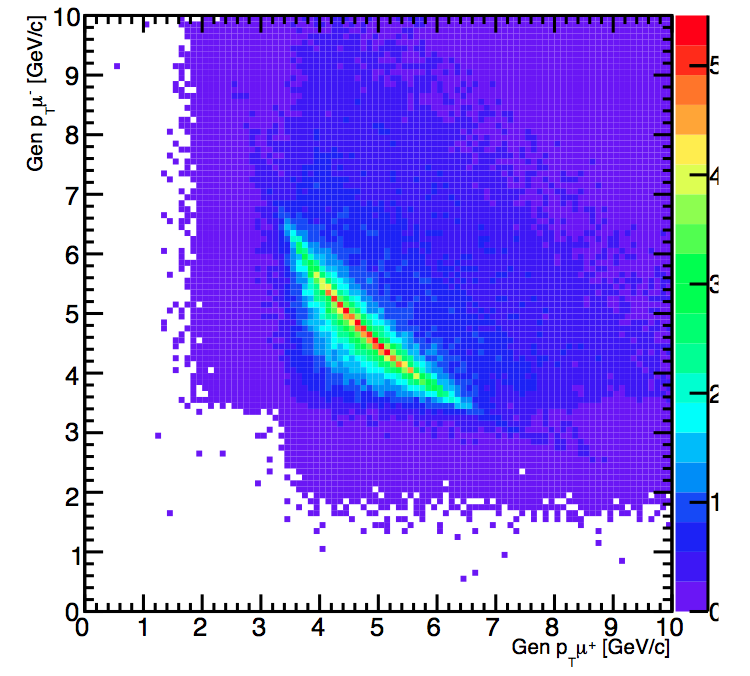
\includegraphics[width=0.50\textwidth]{Chapters/aYield/Gen_mupt_vs_mupt.png}  
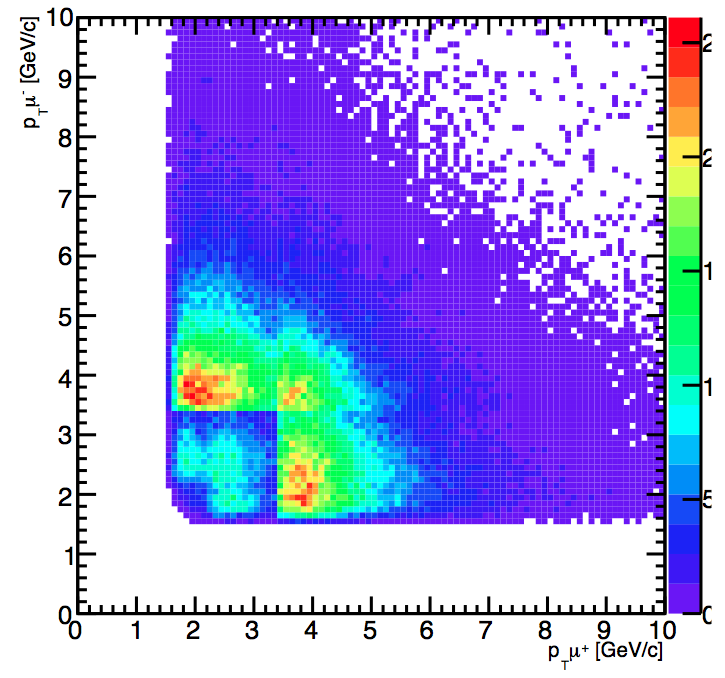
\includegraphics[width=0.48\textwidth]{Chapters/aYield/Data_mupt_vs_mupt.png}  
\caption{2D-distribution of muon \pt\ for generator-level \PgU\ (left)
  and
  PbPb data in the \PgU\ mass range (right).}
\label{fig:twoMuonsPt}
\end{center}
\end{figure}

From Figure~\ref{fig:twoMuonsPt} and the red histograms of
Figure~\ref{fig:massPlotsLooseAndIntermediate}, one can conclude that
cutting on the muons with a \pt\ above 4 \GeVc\ is limiting the available
statistics, although cutting away a large fraction of the background
yield. Additionally, cutting too low in \pt\ adds a lot of background
in the mass plot. Finally, we turn to asymmetric cuts and observe that
the signal amount appears conserved, while some of the background is
rejected. This cut is going to be investigated in more detail.

\subsection{Asymmetric single-muon transverse momentum cuts}


The goal of the analysis being to evaluate the
suppression of \PgU\ mesons in various kinematic regimes (low-\pt,
high-\pt, increasing rapidity) by the means of a nuclear modification
factor, the important figure in our evaluation is the precision with
which this suppression is extracted. The relative uncertainty on the
suppression, that is to mean the statistical uncertainty obtained from
optimizing with the cuts in pp and PbPb data at the same time, is the
factor to be minimised.

% Let us extend the plots in
% Figure~\ref{fig:massPlotsLooseAndIntermediate} with additional \pt\
% asymmetric cuts to look for further improvement. From this point, a
% definitive way to estimate the gains and losses in signal and
% background would be needed.

% \begin{figure}[h]
% \begin{center}
% 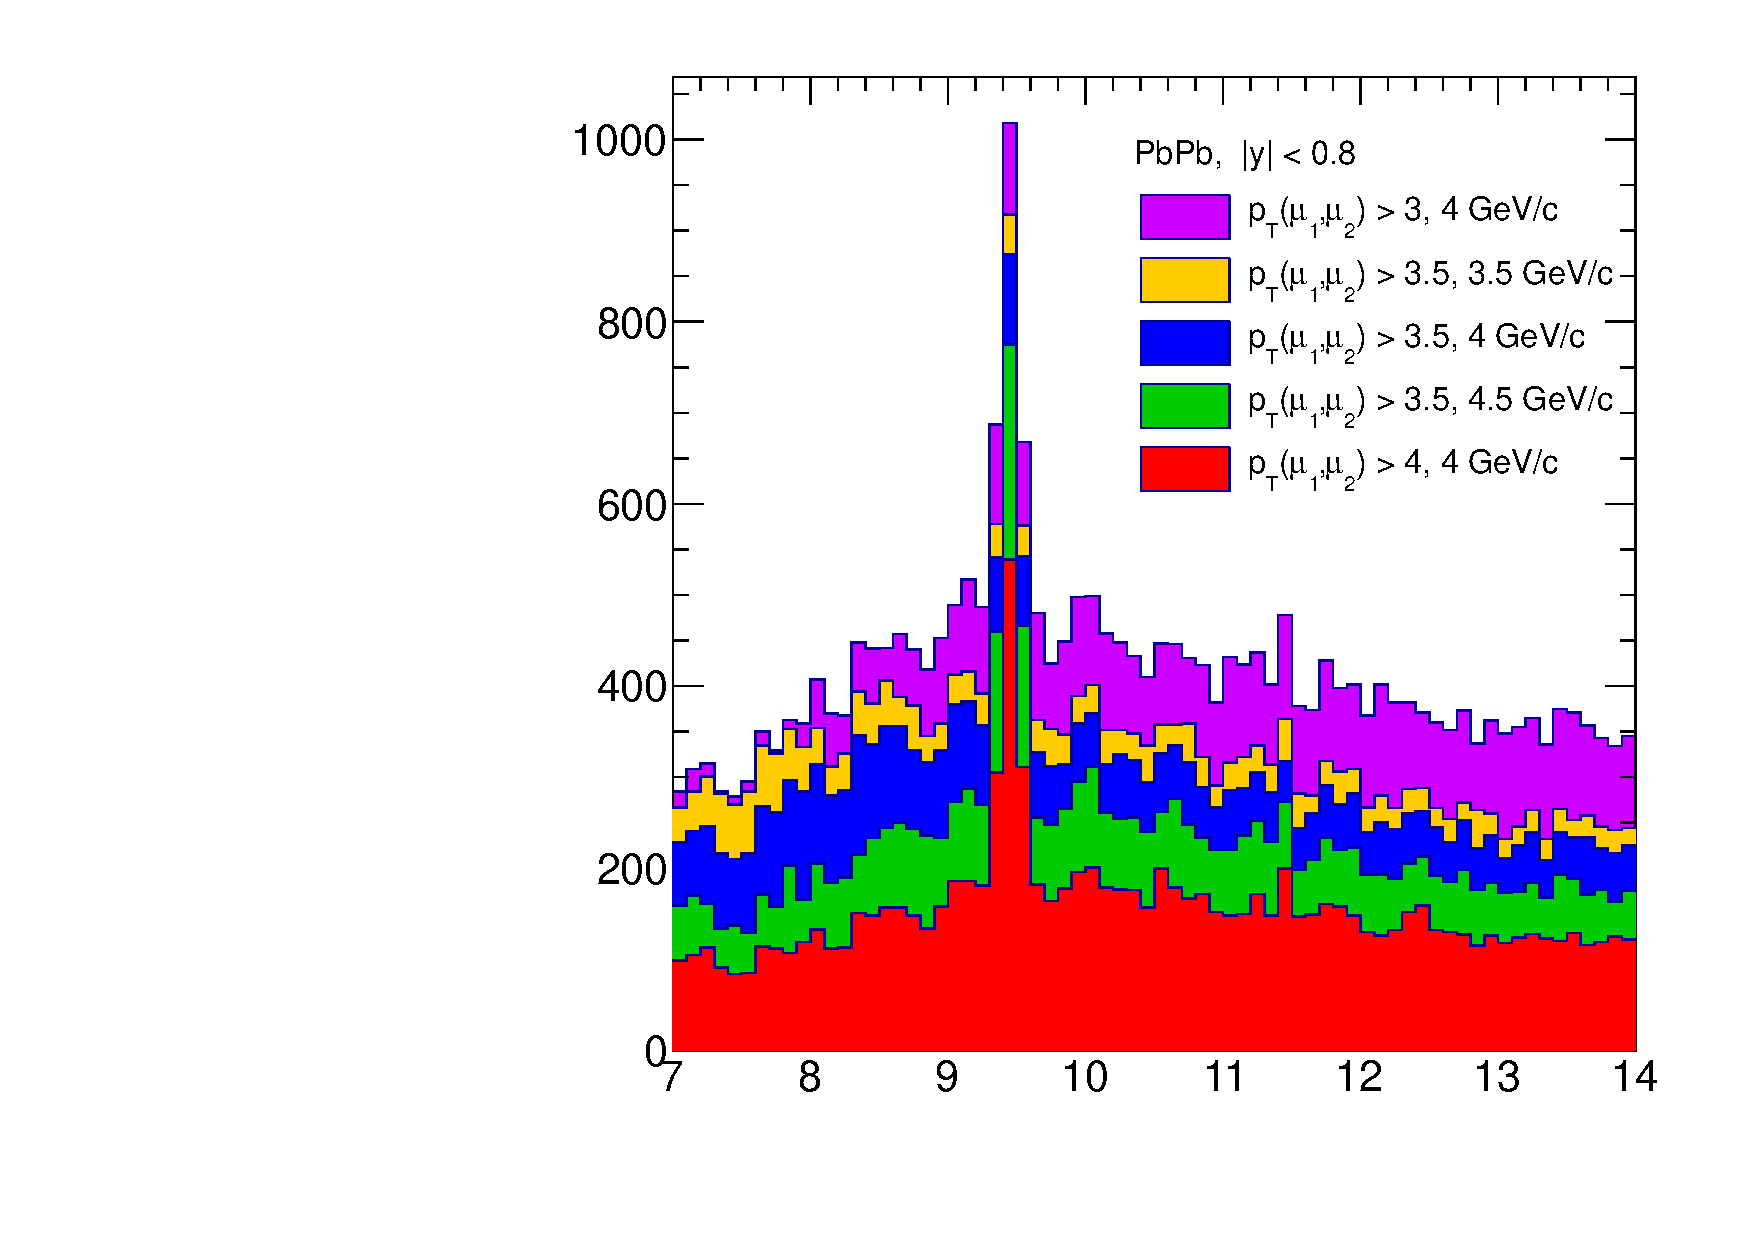
\includegraphics[width=0.3\textwidth]{Chapters/aYield/BarrelMassPlotsMoreBins.pdf}
% 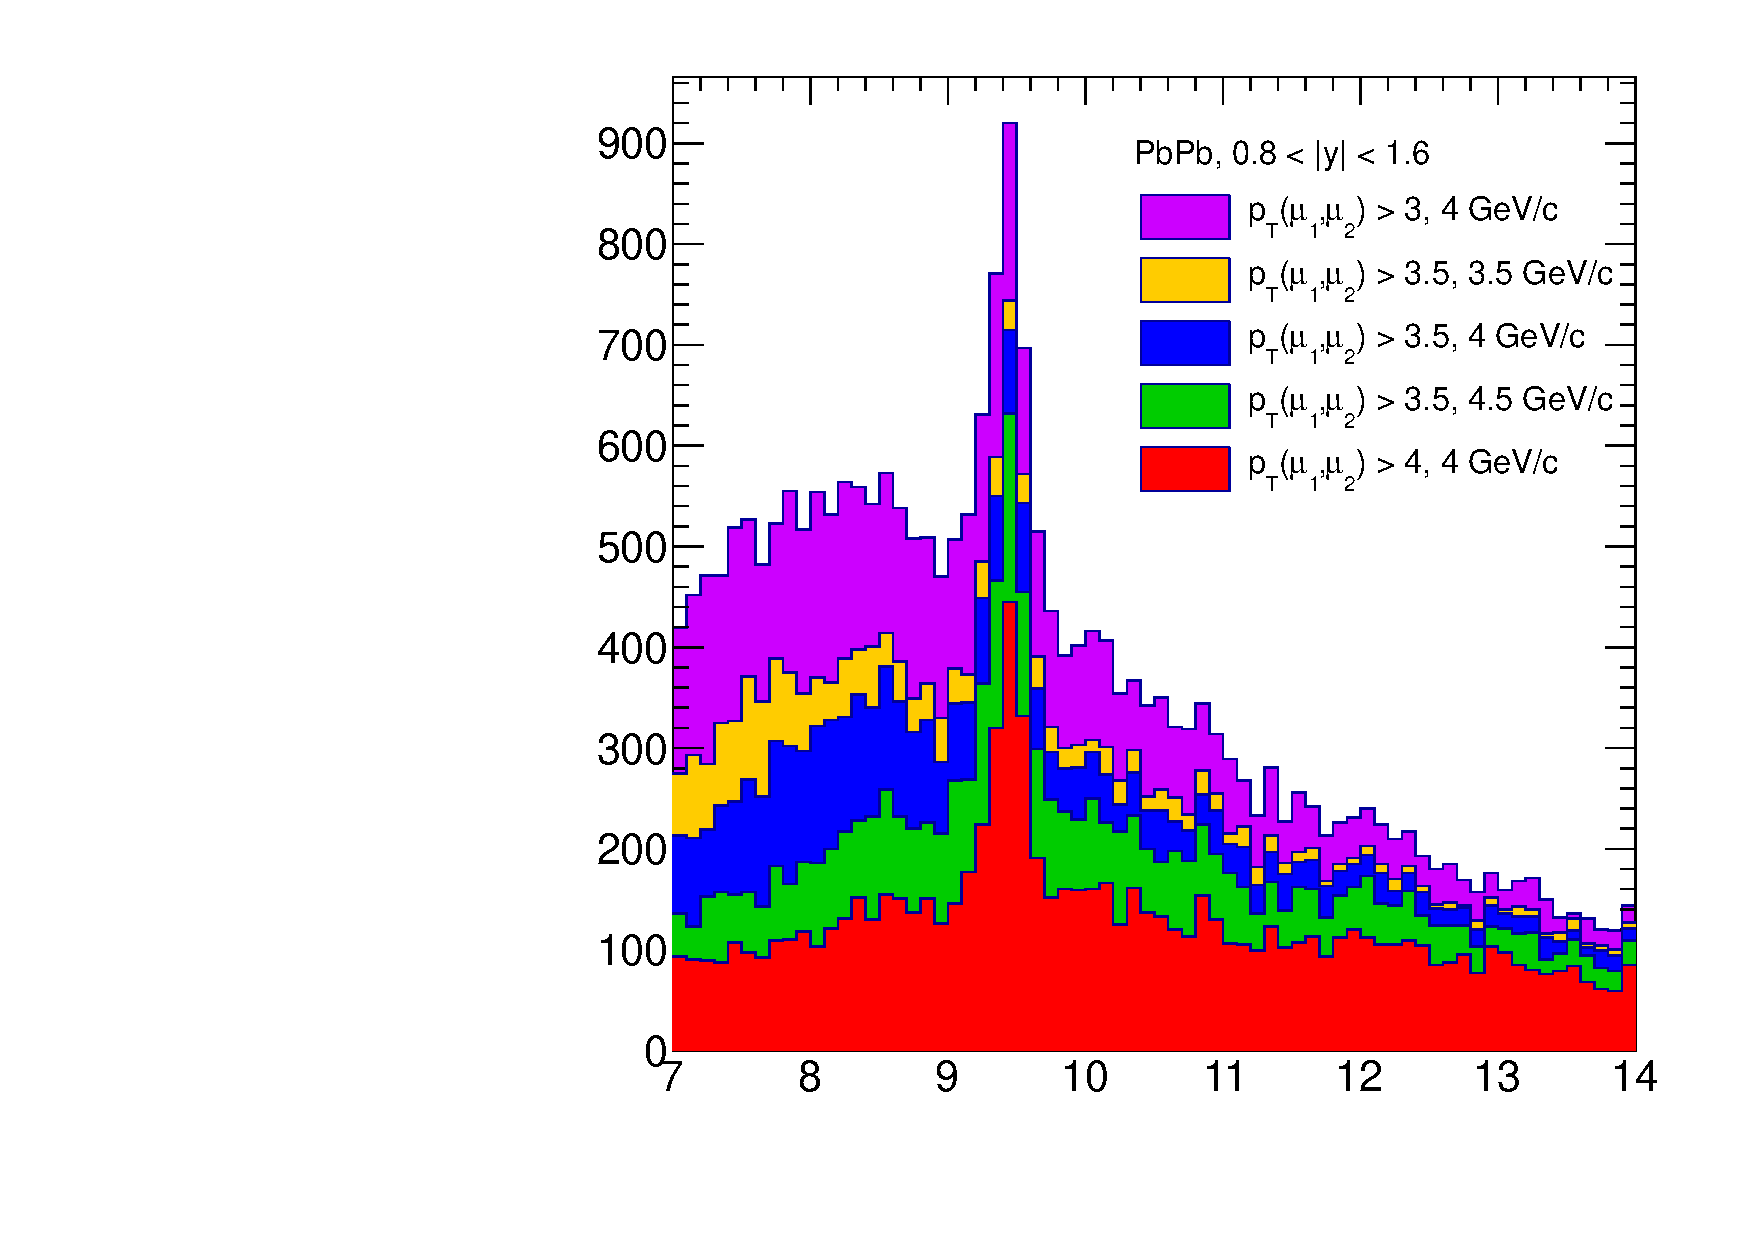
\includegraphics[width=0.3\textwidth]{Chapters/aYield/intermediateRapidityMassPlotsMoreCuts.pdf}  
% 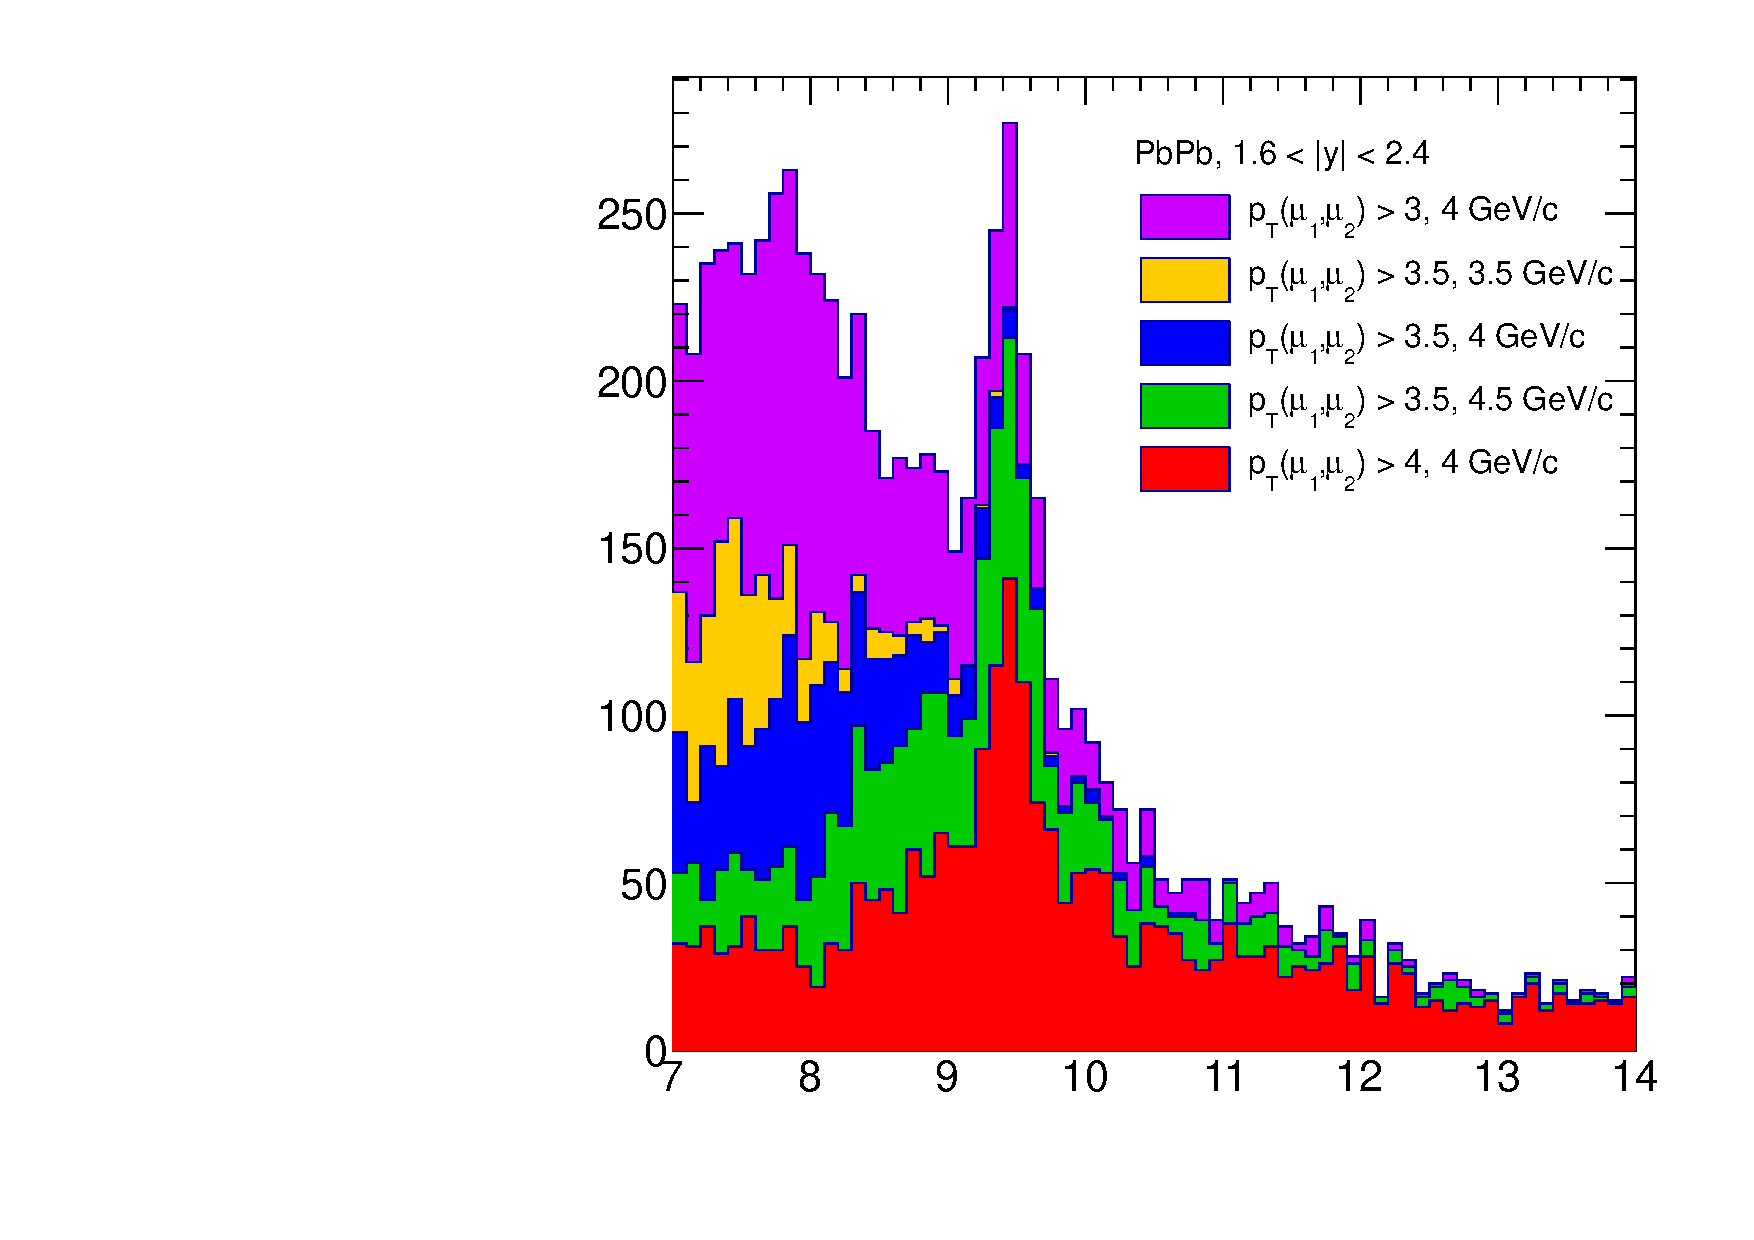
\includegraphics[width=0.3\textwidth]{Chapters/aYield/EndcapMassPlotsMoreCuts.pdf}  
% \caption{Dimuon invariant mass
%   histogram for five different sets of cuts, in three rapidity
%   regions: barrel |y|<1.2 (left), intermediate 1.2<|y|<1.6 (center),
%   endcap 1.6<|y|<2.4 (right). Extension of Figure~\ref{fig:massPlotsLooseAndIntermediate}.}
% \label{fig:massPlotsLooseAndIntermediateMoreCuts}
% \end{center}
% \end{figure}

% The complete list of histograms is now red, yellow, blue (previously
% defined) and:
% \begin{itemize}
% \item[-] \textit{Purple histogram:}~$\pt(\mu(1) > 3 \GeVc\ and
%   $\pt(\mu(2) > 4 \GeVc\ is applied. The background has largely
%   increased compared to all the other case, to the point where it
%   starts to seriously overshoot the signal yield.
% \item[-] \textit{Green histogram:}~$\pt(\mu(1)) > 3.5 \GeVc$ and
%   $\pt(\mu(2)) > 4.5 \GeVc$ is applied. This asymmetric cut seems to
%   reduce background of a certain amount compared to the blue
%   histogram, at the price of shifting it just below the \PgUa\ peak,
%   which would increase the systematic uncertainty on its estimation.
% \end{itemize}

% To make an
% accurate statement from the mass histograms in
% Figure~\ref{fig:massPlotsLooseAndIntermediateMoreCuts} on what would be the best cut for data, one would
% have to use a figure of merit - e.g. the \textit{significance} - in which the signal is
% computed from Monte-Carlo and the corresponding background estimated
% from data sidebands normalized to the mass window where the signal
% was measured. This however would not reproduce the
% signal-to-background ratio seen in PbPb data and would complicate
% significantly the study, since the background shape changes clearly
% from a muon \pt\ cut to another, and from a rapidity region to
% another.
%  However, we can extract the following
% quantity\footnote{further referred to as \textit{composite
%     significance}}:

% \begin{equation}
% \mathcal{S}_c = \frac{S}{\sqrt{S+B}} 
% \end{equation}
% using S from MC extraction (simple counting after applying cuts on a
% reconstructed, simulated signal with no background embedding)
% and using B from the left and right sidebands, thus avoiding biases of
% looking directly at data to judge. Instead of looking directly at the
% output of \signif to infer on the cuts, we'll try to 

In Figure~\ref{fig:massPlotsLooseAndIntermediate}, we followed the
logic of comparing blue and yellow histograms to the red one, where
both muons suffer a \pt\ cut of 4 \GeVc. The next step is to estimate
the statistical increase in signal and background regions, as is done
in Table~\ref{tab:gains}. The increases are formulated in terms of
gains (in percent) with respect to
the red histogram. One can note that both cuts being looser, the gains
in blue and yellow histograms with respect to the red one \textit{are} positive.

The three regions studied are: m$_{\mu\mu}\in$
[9.2, 9.7] \unitMass\ for the signal region,  m$_{\mu\mu}\in$ [7,9.2] and
m$_{\mu\mu}\in$ [9.7,14] \unitMass\ for the background regions,
respectively called 'SB$_{\rm L}$' and 'SB$_{\rm R}$' for left and
right \textit{sidebands}. In the
signal region, the gains are computed with simulated yields.
This procedure allows to avoid any bias in the signal region.

 The cut
tested in the upper part of Table~\ref{tab:gains} corresponds to the
yellow histogram of Figure~\ref{fig:massPlotsLooseAndIntermediate},
while the lower part of the table compares the gains of the blue
histogram of Figure~\ref{fig:massPlotsLooseAndIntermediate}.

When studying the sidebands (first and third columns of
Table~\ref{tab:gains}), one can see that both histograms present
an increase of more than 70 \%\ in every region. The symmetric
cut tested in the upper part of the table (yellow histograms) shows an
increase of more than 100 \%\ on the left
sideband, in all three rapidity bins, and in two of the three rapidity bins of the right sideband. This
indicates that, when reducing of only 500 \MeVc\ the \pt\ threshold
for both muons, the background level is approximately doubled.

For the lower part of the table (blue histogram) where an asymmetric
cut is tested, a smaller increase of 70$\sim$90 \%\ is seen in both
sidebands. This is understood since the \pt\ threshold was reduced on
only one muon. In the same time, the
signal region sees an increase of approximately 20 percent,
consistent between the two cuts tested. This last observation leads us
to conclude that while the background yield varies with the two cuts
tested, the signal is already well maximised. The asymmetric cuts thus
has the advantage of reducing the extra background yield while
maintaining an improved signal yield.

\begin{table}[h]
  \begin{center}
    \begin{tabular}{c|c|c|c}
\hline
      \pt\ $>$ (3.5, 3.5)~\GeVc &Gains in SB$_{\rm L}$ &  Gain in MC Signal&Gain in SB$_{\rm R}$\\
      \hline
      Rapidity interval&m$_{\mu\mu}\in$ [7,9.2]~\unitMass&m$_{\mu\mu}\in$ [9.2,9.7]~\unitMass&m$_{\mu\mu}\in$ [9.7,14]~\unitMass\\ 
      \hline
       $|y| <$  0.8       &101\%& 18.3\%& 101 \% \\
      0.8  $< |y| <$  1.6 &126\%& 22  \%& 79.2\% \\ 
      1.6  $<  |y| <$  2.4 &101\%& 18.3\%& 101 \% \\  
      \hline
      \pt\ $>$ (3.5, 4)~\GeVc  &Gains in SB$_{\rm L}$ &  Gain in MC Signal&Gain in SB$_{\rm R}$\\
      \hline
      Rapidity interval&m$_{\mu\mu}\in$ [7,9.2]~\unitMass&m$_{\mu\mu}\in$ [9.2,9.7]~\unitMass&m$_{\mu\mu}\in$ [9.7,14]~\unitMass\\ 
      \hline
       $|y| <$  0.8       &79.9\%& 17.9\%& 81.3\% \\
      0.8   $< |y| <$  1.6 &96.1\%& 21.5\%& 68.1\% \\ 
      1.6   $< |y| <$  2.4 &79.9\%& 17.9\%& 81.3\% \\ 
      \hline      
      % \pt > 3.5, 4.5 &Gain in  m$_{\mu\mu}\in $ [7,9.2[ &  Gain in MC Signal &Gain in m$_{\mu\mu}\in $ [9.7,14] \\
      % \hline
      % \hline
      %  $|y| <$  0.8       &40.5\%& 15.3\%& 45.4\% \\ 
      % 0.8   $< |y| <$  1.6 &47.2\%& 18.5\%& 43.4\% \\
      % 1.6   $< |y| <$  2.4 &40.5\%& 15.3\%& 45.4\% \\
      % \hline
      % pt = 3, 4 &Gain in m$_{\mu\mu}\in $ [7,9.2[ &  Gain in MC Signal
      % &Gain in  m$_{\mu\mu}\in $ [9.7,14] \\
      % \hline
      % \hline
      %  $|y| <$  0.8       &109\%& 22.4\%& 166\%\\ 
      % 0.8   $< |y| <$  1.6 &206\%& 32.7\%& 125\%\\
      % 1.6   $< |y| <$  2.4 &109\%& 22.4\% & 166\%\\
    \end{tabular}
  \end{center}
  \caption{Added values from releasing the muon \pt cuts, in symmetric
    and asymmetric cuts, in PbPb data and MC. Added values are computed as relative to the
    standard tight cut (\pt > (4~\GeVc, 4~\GeVc)). The signal region
    is computed using MC simulations.}
\label{tab:gains}
\end{table}

% The cut represented by purple histograms in
% Figure~\ref{fig:massPlotsLooseAndIntermediateMoreCuts} represent the
% last line in Table~\ref{tab:gains}. It shows a $\simeq$ 25\% increase
% in signal, at the price of a 100 to 200 \% gain in background. This
% possibility has been discarded in the following because of the severe
% loss of precision it will bring to the PbPb yields. In terms of what
% would be the smallest gain in background, the cut represented in the
% third line (green histogram, $\pt(\mu(1)) > 3.5 \GeVc$ and
% $\pt(\mu(2)) > 4.5 \GeVc$). Looking at the histograms however, the
% background looks shifted below the mass peak, compared to the blue
% histogram. This will result in larger systematic uncertainties in
% the yield extraction, especially at large rapidities where the
% background seems to accumulate under the \PgUa\ peak, making it hard
% to resolve accurately. Finally the three options we're left with are blue, red and yellow histograms.

% From Table~\ref{tab:gains}, one can conclude that be

The figure of merit used in the following is referred to as
\textit{fit significance}, and is defined as the ratio of fitted yield
over fitted error:
\begin{equation}
\Sigma_{\rm{fit}} = \frac{\NFit}{\sigma(\NFit)} ,
\end{equation}
where \NFit\ stands for the extracted number of events from the \PgUa\
resonance when performing a maximum likelihood estimation on data, and
where $\sigma$(\NFit) comes from the 1-$\sigma$ error on \NFit\ estimation.% \footnote{Obtained after maximising the
  % likelihood function, Appendix~\ref{chap:stats}}. 
The method
used in fitting corresponds to that of Section~\ref{sec:sigext}.%  The
% probability density function (PDF) used for fitting the signal is a
% linear combination of two Crystal Ball functions~\cite{SLAC-R-236},
% while the background is described by the product of a real-valued
% error function~\cite{math:erf} and an exponential function. Both components
% of the \CB\ function are assured to pick the same values for the
% radiative tail parameters $\alpha$ and $n$, but are not constrained in
% any way for this study.

The significance is computed in all three cuts for every bin of the
analysis \textit{vs.} \Npart, \pt, \y. The \pt\ and \y\ bins are
investigated twice: once when looking into pp data, and looking into
PbPb data. The output of all the significances extracted is reported
in Figure~\ref{fig:significance}.
\begin{figure}[h]
\begin{center}
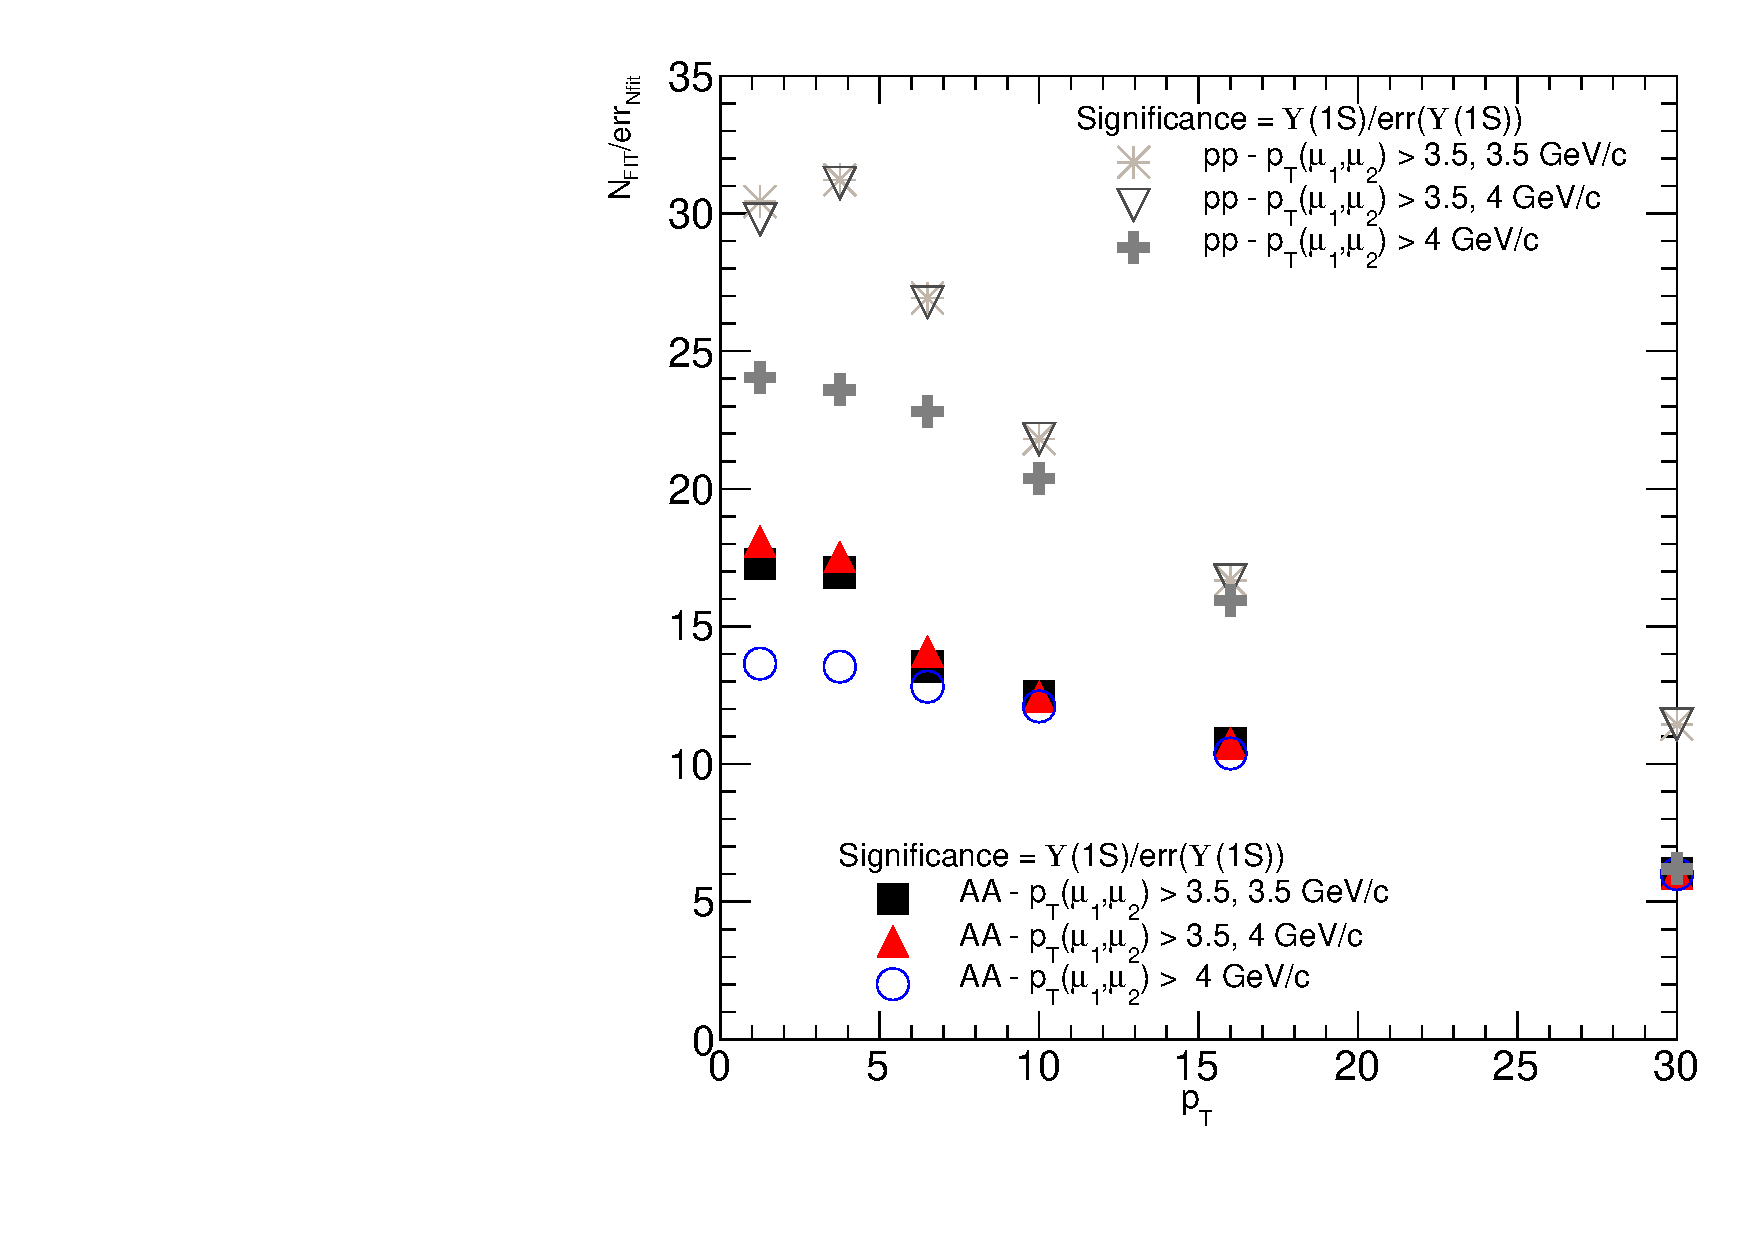
\includegraphics[width=0.48\textwidth]{Chapters/aYield/signif_pp1_pbpb1_pt1_rap0.pdf}
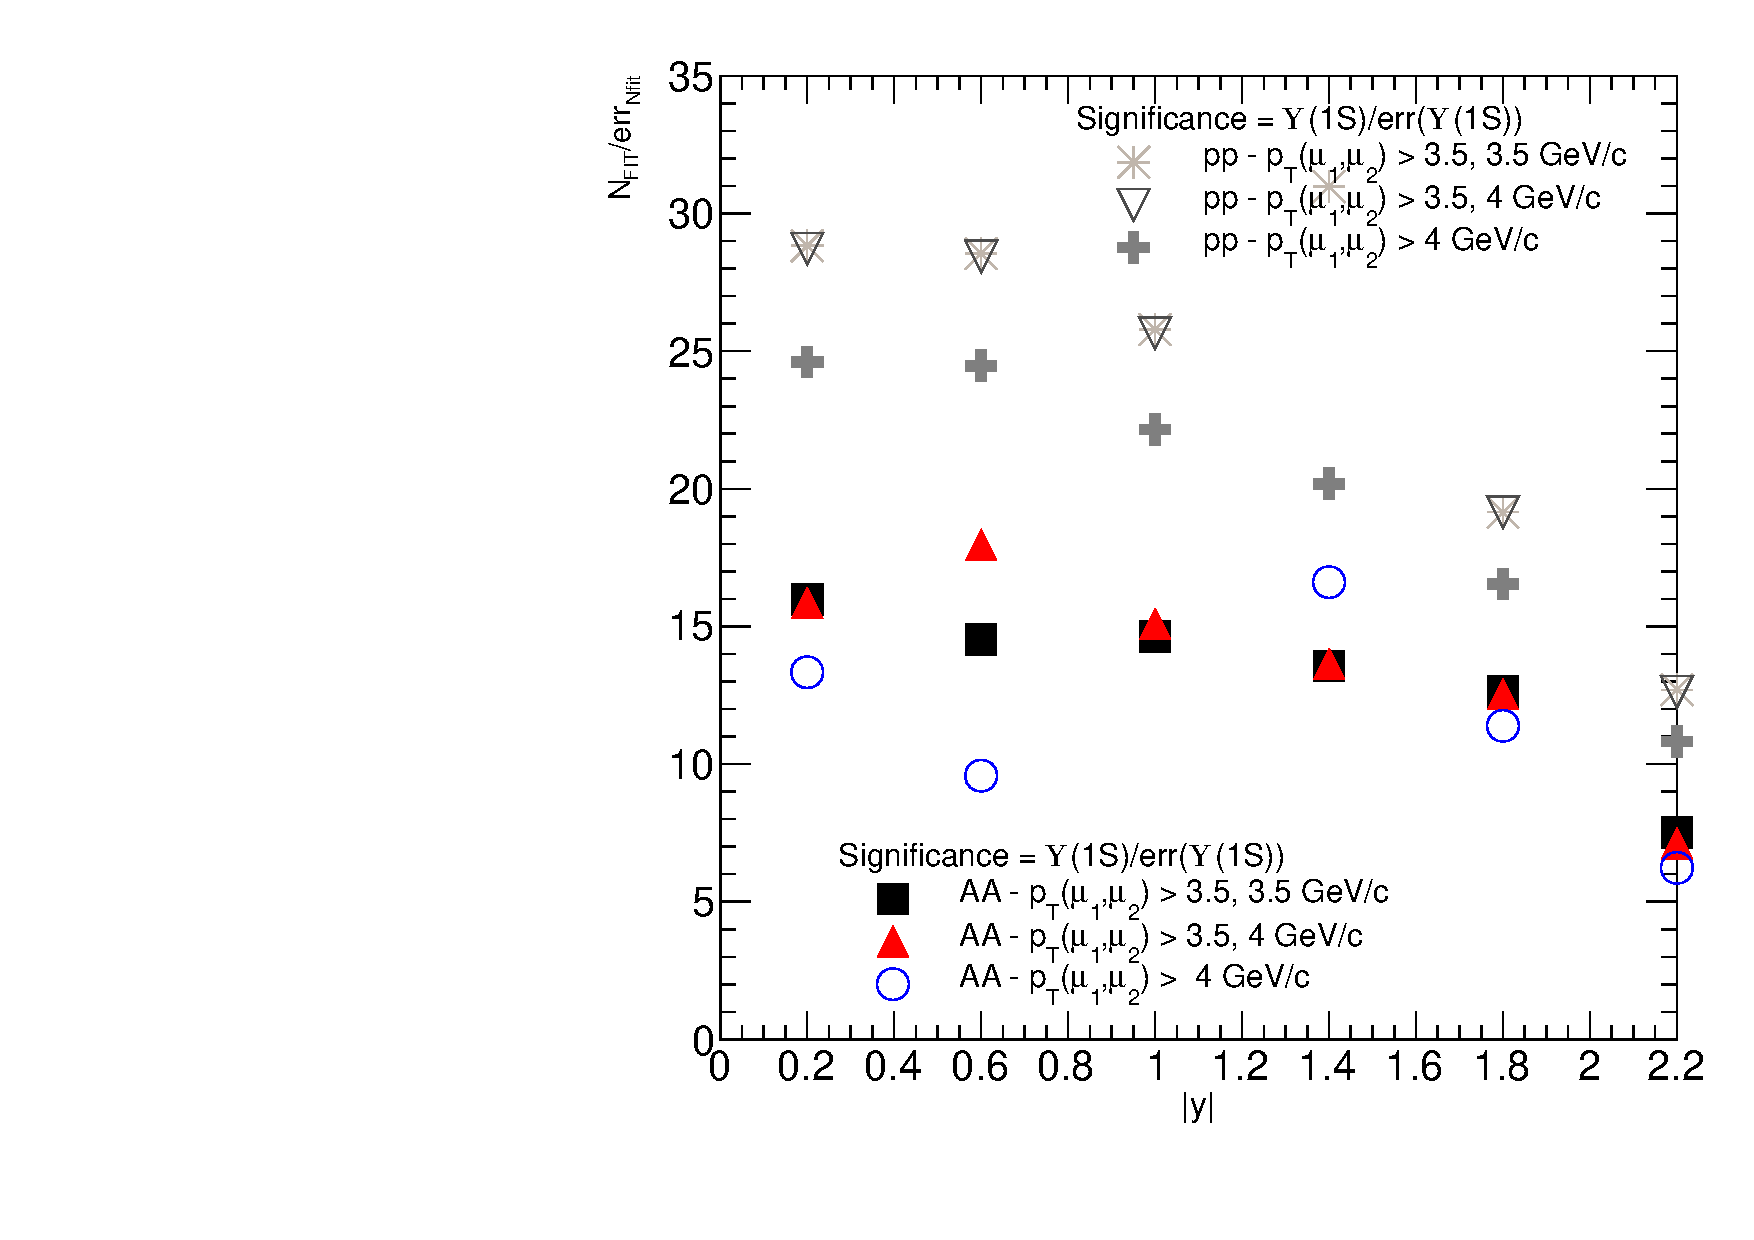
\includegraphics[width=0.48\textwidth]{Chapters/aYield/signif_pp1_pbpb1_pt0_rap1.pdf}
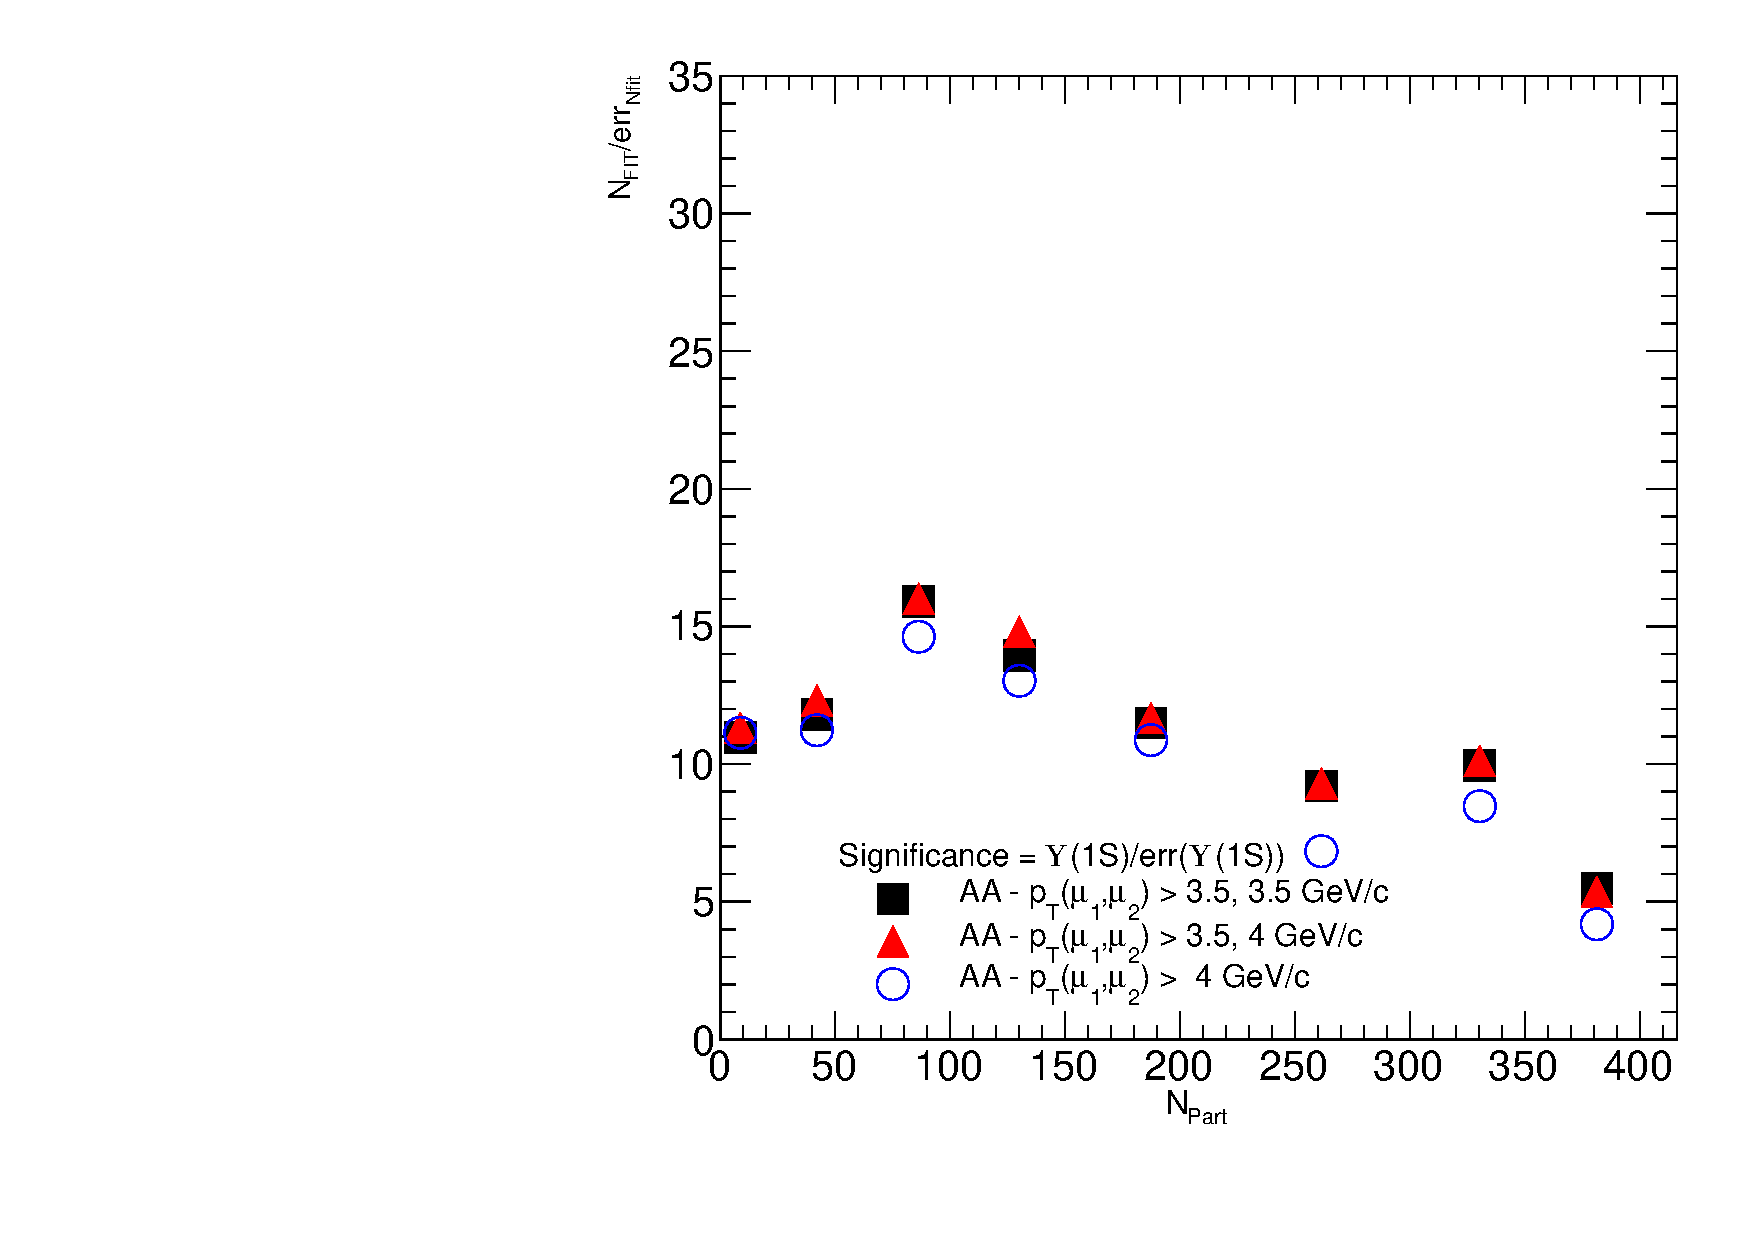
\includegraphics[width=0.49\textwidth]{Chapters/aYield/signif_pp0_pbpb1_pt0_rap0.pdf}
\caption{Signal over error ratios (i.e. fit significances) for each bin of the \PgUa\
  analysis. First, transverse momentum binning; Second: rapidity
  binning; Third: \Npart\ binning. Open triangles and filled
  triangles denote the most satisfactory cut ($\pt{}_{1} > 3.5~\GeVc$ and
$\pt{}_{2} > 3.5~\GeVc$) in $pp$ and PbPb data, respectively.}
\label{fig:significance}
\end{center}
\end{figure}

From the significances, a first important observation is the clear
gain in precision when releasing the muon \pt\ cuts from 4 \GeVc to
3.5 \GeVc for one muon. It was decided to
do the study with settings as close as possible to what the final analysis
is, to get a clear handle of the gain in precision in outcome of this
study. Second, although the gains in PbPb data are of the order of 4
$\sigma$ in the low-\pt\ bins, the relative precision obtained in the
nuclear modification factor will be largely increased thanks to the
gain in pp statistics, where the background is smaller and therefore easier to
control. In the two lowest-\pt\ bins, the pp statistics is increased
of 10 to 12 $\sigma$ from the grey symbols in
Figure~\ref{fig:significance}, which is very encouraging. % In PbPb data, the
% gain is present over all centrality ranges, allowing for an extra
% peripheral bin 70-100\% as shall be presented
% in Section~\ref{sec:sigext}. 



In summary, the symmetric 3.5
\GeVc\ cut does not seem to increase the significance; however, we have
seen in previous mass plots that this cut enhances the low mass part
of the background. In the same time, the asymmetric cut does a better
job in the sideband regions, while the signal is improved. As a
conclusion, it was 
decided to use the asymmetric cut $\pt{}_{1} > 3.5~\GeVc$ and
$\pt{}_{2} > 3.5~\GeVc$ as the kinematic cut for the \PgUa\ signal
extraction. In the case of the \PgUb\ and \PgUc\, it can
be shown that both signals are consistently low, the \PgUc\ remaining
unobserved in heavy ion collisions, and the \PgUb\ peaking at a
3~$\sigma$ significance level. In these conditions, it was decided to keep a
symmetric cut of \pt\ > 4 \GeVc\ for the \PgUb,~\PgUc\ analyses.
\vspace{0.5em}
 \begin{center}
\fbox{
  \parbox{0.9\textwidth}
  {\textsf {In this Section, I have shown some aspects of my study of
      the low-momentum muons in CMS. We have seen the following
      points:
      \begin{itemize}
        \item[-] A large fraction of \PgU\ events have at least one
          muon below the previously used cut $\pt > 4~\GeVc$,
        \item[-] While the magnetic field in the barrel naturally places a lower \pt\
          limit at $\pt(\,\vert\eta\vert\,<1.2) \approx 3.4~\GeVc$,
          going lower in \pt\ in the endcaps does not
          enhance the \PgU\ data signal, and includes unwanted
          background events,
          \item[-] Various \pt\ constraints were tested on each muons
            and led
            us to consider asymmetric muon \pt\ cuts as the best
            choice to optimise the \PgUa\ signal,
          \item[-] This strategy however is not sustainable in the
            case of \PgUb, which suffers more suppression.
      \end{itemize}
    With these points covered, the sets of kinematic cuts for each
    \PgU\textrm{(nS)} are:
    \vspace{0.1cm}
    \begin{center}
      \begin{tabular}{p{1.3cm}p{2.5cm}p{3.2cm}p{3.2cm}}
        \hline
        \PgUa & ``loose cut'' & p$_{T}^{\mu_1} > 3.5$~\GeVc & p$_{T}^{\mu_2} > 4$~\GeVc \\ 
        \PgUb, \PgUc\ & ``tight cut'' & p$_{T}^{\mu_1} > 4$~\GeVc & p$_{T}^{\mu_2} > 4$~\GeVc \\
        \hline    
      \end{tabular}
    \end{center}  
    \vspace{0.1cm}
      In the following section, the fitting strategy is
      presented. After a short review of the lineshape study motivated by the signal peak
      resolution varying with rapidity, we then turn to the resulting
      \PgU\ yields. A large
     \PgUa\ significance in every bin comes to confirm the validity of
      the chosen cuts, before the systematic uncertainties are studied.}
  }
}
\end{center}
\section{Signal extraction}
 \label{sec:sigext}

\subsection{Fits to the invariant mass spectrum}
 \label{sec:sigext_fits}
% From now on, the following kinematic cuts on the single-muon
% transverse momentum are applied:
% \begin{center}
%     \begin{tabular}{p{1.3cm}p{2.5cm}p{3.2cm}p{3.2cm}}
% \hline
% 1S & ``loose cut'' & p$_{T}^{\mu_1} > 3.5$~\GeVc & p$_{T}^{\mu_2} > 4$~\GeVc \\ 
% 2S, \PgUc\  & ``tight cut'' & p$_{T}^{\mu_1} > 4$~\GeVc & p$_{T}^{\mu_2} > 4$~\GeVc \\
% \hline    
% \end{tabular}
% \end{center}
The raw yields were extracted by fitting the dimuon invariant mass spectrum in the range 
\begin{equation}
7.5 \leq m_{\mu\mu}\ [{\rm GeV}/c^2] < 14\ . \nonumber
\end{equation}
% In previous analyses, the
%     low-mass limit was 7 GeV/c$^{2}$. However, when applying the tight
%     cut to the lowest
%     p$_{T}$ bin, only few events in the continuum below 8
%     GeV/c$^{2}$ can be seen due to kinematical constraints. This led
%     to restrict the mass range of to 7.5-14 GeV/c$^{2}$ for all bins.


Yield extraction makes use of an unbinned maximum likelihood
technique. Using standard minimisation tools of
RooFit~\cite{Verkerke:2003ir}, the data is fitted with a user defined
probability density function (PDF) in an attempt at minimising the
negative log-likelihood $-\textrm{ln}\mathcal{L}$ of the distribution. % The procedure used here is sometimes called extended, for
% it treats the normalisation of each signal 
% This unbinned method allows 
% A user
% defined  (pdf) is used to fit the data, and the maximum
% likelihood method (using standard tools of RooFit) seeks to minimise
% the negative log likelihoo
%  extended unbinned minimum negative log-likelihood fitting procedure. 
%%
%%As detailed in Monte Carlo studies (see Appendix~\ref{sec:FSRfits}), 

The $\PgU$ resonances are commonly modeled experimentally by a Crystal Ball (CB) function.
The Crystal Ball function consists of a Gaussian distribution and of a power law on the
low-mass tail accounting for muon final state radiation. It is given by
%\begin{linenomath}
\begin{equation} \label{CrystalBall}
  \CB(x;\bar x,n,\alpha,\sigma) = N \cdot \left\{
  \begin{array}{ll}
    \exp(- \frac{(x -\bar x)^2}{2 \sigma^2})      & \mbox{for } \frac{x - \bar x}{\sigma} > -\alpha \\
    A \cdot (B - \frac{x - \bar x}{\sigma})^{-n}  & \mbox{for } \frac{x - \bar x}{\sigma} \leq -\alpha \,,
  \end{array}
  \right.
\end{equation}
%\end{linenomath}

where
%\begin{linenomath}
\begin{eqnarray}
  A & = & \left(\frac{n}{\left| \alpha \right|}\right)^n \cdot \exp\left(- \frac {\left| \alpha \right|^2}{2}\right) \,, \nonumber \\
  B & = & \frac{n}{\left| \alpha \right|} - \left| \alpha \right| \,. \nonumber
\end{eqnarray}
%\end{linenomath}
Since this analysis spans various \pt\ and rapidity regions, the
resolution of the peaks may change from a bin to another one. This could
already be sensed in the three panels
of Figure~\ref{fig:massPlotsLooseAndIntermediate}. The previous analyses
of \PgU\ in heavy ion collisions~\cite{torsten,HIN-11-007,11-011} used a Crystal
Ball function for each \PgU\ state, fixing its width and final state
radiation tail to values obtained from MC simulations. In the next
Section~\ref{sec:sigext_FSR} I present an equivalent study. The main difference with
previous works comes from the fact that our fine binning in
rapidity and \pt\ motivates to tune the signal shape parameters
independently for each bin, instead of fixing them to a 'minimum bias'
value.


For the sake of presenting the full fitting strategy before looking at the
results of the lineshape study in detail, I want to anticipate and
present the total signal and background PDF used in fitting data. A sum of two Crystal Ball functions was preferred over a single
Crystal Ball % (or, a Crystal Ball plus a Gaussian) 
because of the varying mass resolution with increasing
di-muon rapidity. The resulting signal PDF used for the  $\PgUa$ resonance
is defined as

\begin{equation}
\Sigma_{1S}\left( m_{\mu\mu} ; m_{0}, n, \alpha, \sigma_{0}, f, x\right) = f\cdot \CB_{1}\left( m_{\mu\mu}
  ; m_{0}, n, \alpha, \sigma_{0} \right) + \left(1-f\right)\cdot
\CB_{2}\left(  m_{\mu\mu};m_{0},n,\alpha,x\cdot\sigma_{0}\right) \ .
\label{eq:DoubleCrystalBall}
\end{equation}


In order to reduce the number of free independent parameters in the
fit, we assume the values of $m_0$ and final state parameters $n$, and
$\alpha$ to be shared by both Crystal Ball functions. 
The six fitting parameters (omitting the peak normalisation, see
further) for $\Sigma_{1S}$ are therefore the Gaussian peak mean and
width $m_0$ and $\sigma_{0}$,
Crystal Ball parameters $n$ and $\alpha$ for final state radiation,
the ratio of the two Crystal Ball widths $x$, and the ratio of the two
Crystal Ball normalisations, $f$.
% Appendix~\ref{sec:FSRfits}
% Since the widths of the states, as well as the final state radiation
% parameters, vary with rapidity, it was decided to perform a study in
% order to understand better and eventually constrain these
% parameters. 

The fitting was hence performed first on MC reconstructed
peaks, that yielded
 separate results from PYTHIA (for pp) and the samples embedded in
 HYDJET (for PbPb). As a result, pp and PbPb peaks have separate constraints.

Regarding the PDF of the \PgUb\ and \PgUc\ excited states, the
parameters $n$, $\alpha$, $f$ and $x$ are set to be identical to those
of the \PgUa\ PDF, Eq.~(\ref{eq:DoubleCrystalBall}). In order to account for the
mass-dependent detector resolution, we shall assume that both the
width $\sigma_{nS}$ and the mass $m_{nS}$ scale like 

%
  \begin{eqnarray}
    m_{nS} & = & m_{0} \cdot \frac{m^{nS}_{PDG} }{m^{1S}_{PDG}}  \\
    \sigma_{nS} & = & \sigma_{0} \cdot  \frac{m^{nS}_{PDG}
    }{m^{1S}_{PDG}}  \nonumber \ .
    \label{eq:massRatio}
  \end{eqnarray}
%

With this prescription, the $\PgU$(nS) PDFs read
%\begin{eqnarray*}
\begin{equation}
\Sigma_{nS}\left( m_{\mu\mu} ; m_{0}, n, \alpha, \sigma_{0}, f, x\right) =
\Sigma_{1S}\left( m_{\mu\mu}
  ; m_{0} \cdot \frac{m^{nS}_{PDG} }{m^{1S}_{PDG}}, n, \alpha, \sigma_{0} \cdot  \frac{m^{nS}_{PDG} }{m^{1S}_{PDG}}, f, x \right) \ .
  \end{equation}
%  \\

  The 5 parameters $n$, $\alpha$, $f$, $\sigma_{0}$, $x$ are
  determined from pure signal Monte Carlo simulations in Section~\ref{sec:sigext_FSR}, with distinct
  constraints for pp and PbPb signals. The mean
  parameter $m_0$ is kept free in the fit to the data to account for varying
  muon momentum scale inaccuracies over various areas of the detector.
%
Once these are fixed, the signal  $\Sig$ is defined as a weighted sum of the $\PgUa$, $\PgUb$, and $\PgUc$ PDF,\footnote{In the following, we shall use for clarity the shorthand notation 
$\Sig(m_{\mu\mu}; \NFitOneS, \NFitTwoS, \NFitThreeS, m_{0})\equiv\Sig(m_{\mu\mu}; \NFitOneS, \NFitTwoS, \NFitThreeS, m_{0}\ \big|\ n, \alpha, \sigma_{0}, f, x)$.}
%%
%\begin{linenomath}
\begin{equation} \label{eq:TheSignalPDF}
 \Sig(m_{\mu\mu}; \NFitOneS, \NFitTwoS, \NFitThreeS, m_{0} \big|\ n, \alpha, \sigma_{0}, f, x)
 = \\ \NFitOneS\cdot\Sigma_{1S}\left( m_{\mu\mu} \right)  +
 \NFitTwoS\cdot\Sigma_{2S}\left( m_{\mu\mu} \right)  +  \NFitThreeS\cdot\Sigma_{3S}\left( m_{\mu\mu} \right) \ .
\end{equation}
%\end{linenomath}
%%
where the raw yields $\NFitOneS$, $\NFitTwoS$, $\NFitThreeS$ and
$m_{0}$ are left as free parameters in the fit to the data sample.%  The
% fixed parameters will be released to compute systematic uncertainties
% in Section~\ref{sec:sigext_vars}. %\ref{sec:fitvariations}. 
The fits are performed on opposite-charge di-muon pairs. 
The signal in data lies on top of a continuum of events identified as
background showing a smooth kinematic increase saturating slightly below the \PgU\ mass.

The typical exponentially falling mass spectrum is multiplied by
an error function  rendering the kinematic turn-on arising from the
single muon \pt\ selection. 

The background model is formed of a real-valued Error function
multiplied by an exponential, and used for the PDF of the background shape, $\B$,
% 
\begin{equation}
\B \left( m_{\mu\mu}; \mu, \sigma, \lambda \right)  =
\exp\left( { -\frac{m_{\mu\mu}}{\lambda}} \right) \cdot \left(1  +
  \text{Erf}  \left(  \frac{m_{\mu\mu} - \mu}{\sigma}  \right) \right)
\ .
\label{eq:TheBackgroundPDF}
\end{equation}
It depends on three parameters
left free in the fitting with this nominal procedure:
%
\begin{itemize}
\item{The kinematic turn-on parameter $\mu$, at which the error
    function starts increasing, }
\item{The width $\sigma$ of the normal distribution from which the error function is
    derived,}
\item{The decay constant $\lambda$ of the exponential function.}
\end{itemize}
%
The normalization $\NBkgd$ comes as an extra fitting parameter.
 As a result, the fit function $\mathcal{F}$ can be summarized as the sum
of signal events and background events:
\begin{eqnarray}
  \F(m_{\mu\mu} ; \NFitOneS, \NFitTwoS, \NFitThreeS, \NBkgd, m_{0},
  \mu, \sigma, \lambda) &=& \\
\Sig(m_{\mu\mu}; \NFitOneS, \NFitTwoS, \NFitThreeS, m_{0}) 
  + \NBkgd \cdot \B(m_{\mu\mu};  \mu, \sigma, \lambda)
  \nonumber \\
  &&  \label{eq:ThePDF}
\end{eqnarray}


Variations on signal and background
shapes were also performed and are used to estimate the systematic
error on the yields, as discussed in Section~\ref{sec:sigext_vars}.
\subsection{Signal lineshape study}
%
\label{sec:sigext_FSR}

The Monte Carlo samples used in the following paragraph are a set of \textsc{PYTHIA}
samples for $\PgUa$ decaying to muons. One of them is a pure signal
sample, while the other one is embedded in a generated sample of events mimicking
the heavy-ion environment, simulated with \textsc{HYDJET}.% The decay muons may undergo a poorer
% reconstruction than in a context of pure signal, so this sample is
% preferred over pure \textsc{PYTHIA} to study the detector effects on the mass
% lineshape and momentum resolution. The muon momentum resolution study
% is documented in another section. 

The radiative decay $\mu
\rightarrow \gamma\mu$ further denoted as \textit{final state
  radiation}~is
carried by \textsc{PHOTOS}, and corresponds to muon
bremsstrahlung. Effects of the muon energy loss on the $\Upsilon$ mass lineshape have
already been studied in \cite{CMS-PAS-BPH-12-006},
in the context of the 7 TeV $\Upsilon$ cross section measurement in pp
performed by CMS. There, a study of the
reconstructed mass and error from track error matrices was
performed, in the rapidity range $|$y$_{\mu\mu}| <$ 0.6. The photon
radiation was also refined with the
computation of probability for photon radiation at a given
$E_{\gamma}$ in QED. Given the statistical and kinematical reaches of
the data samples used in this analysis though, a similar study is out of scope.

In the context of the present analysis, the events are split in
classes of dimuon rapidity extending to the limits of the muon
spectrometer's reach. Hence, the observed peak resolution is
reflecting detector effects coming from parts of the detector which
can be different in terms of efficiency and material budget, making
the resolution varying with rapidity. Furthermore, the resolution of
the dimuon mass peak integrated over all rapidities is a convolution
of resolutions belonging to separate parts of the detector.  We then
studied the resolution and final state radiation with a large
simulation sample used to further constrain the fitting technique, as
mentioned in~\ref{sec:sigext_fits}. The binning applied hereafter follows the one used in the analysis of
$\PgUa$ as well as that of excited states, to get reasonable
estimations of the mass lineshape in both cases. This binning is
reported on page~\pageref{binning} of Section~\ref{subsec:ptbins}. As
said above, this is motivated by the mass resolution varying with
rapidity seen in fits, and the poor stability of mass fits
when releasing constraints on some of the signal shape parameters.

The outcomes of this study are:
\begin{itemize}
\item{Crystal Ball tail parameters
    $\alpha_{CB},n_{CB}$ varying with increasing rapidity,}
\item{necessity for adding a signal p.d.f. for varying resolution in
    bins which are inclusive over rapidity (i.e. $p_{T}$ bins),}
\item{correlations in some fit parameters that were taken care
    of when replacing the second width $\sigma_{2}$ with a scaled
    parameter to $\sigma_{1}$, $x_{{\rm scale}} = \sigma_{2}/\sigma_{1}$.}
\end{itemize}

The functions tried for fitting are: Gaussian, double Gaussian (with
varying widths), Crystal Ball, double Crystal Ball, Crystal Ball plus
Gaussian (varying widths). The double Crystal Ball signal function
was defined in Equation~\ref{eq:DoubleCrystalBall}. The choice
retained for FSR studies is the double Crystal Ball, as can be seen in
figures below. The Crystal Ball + Gaussian seemed like a sufficient
choice at first, eventually discarded because of a poor description
at high-mass and pole mass. 

The minimum-bias fit is reported in the following Figure
\ref{fig:fsrMBFitPyquen} and the fits to all analysis bins are
reported in Figures \ref{fig:fsrFitPyquenPt} to
\ref{fig:fsrFitPyquenRap}. A line is added
to the fit, to account for spurious and misreconstructed
muons. Although the event selection is supposed to remove most of
them, the embedding procedure can alter the reconstruction of muon tracks
overall. This additive component in the simulation
signal is shown not to exceed 2 percent of the total simulated
statistics available. 


\begin{figure}[h]
\begin{center}
\includegraphics[width=0.7\textwidth]{Chapters/aYield/MCpars_Pyquen_cent0M100_bkgModel0_sigModel4_muonEtaM240240_muonPt350M400_dimuPt0005000_dimuY000240_trkRot0_constrain0_fsr0_sigma0_ref0_pulls.pdf}  
\caption{Minimum-bias fit of $\Upsilon$(1S) mass from a simulated
  sample embedded in events generated with HYDJET. The total fit is
  displayed in blue. The yellow and green curves correspond to the two
Crystal Ball functions added together. The red line takes a residual
part of the simulation sample into account, coming
from background simulation.}
\label{fig:fsrMBFitPyquen}
\end{center}
\end{figure}


Sanity checks on fits were performed with the help of likelihood
scans (cf. Figure \ref{fig:likelihoodScanExampleMinBias} for the Minimum Bias
example, and Figure \ref{fig:likelihoodScanExampleHiRap} for the
$2.0 < \vert\y\vert < 2.4$), i.e. projection of the obtained (negative) log-likelihood on
the axis of a given parameter. This allows to see how the fits are
performing with respect to individual fit parameters, but also gives information on the non-linearities
brought into the model. The scans yielded very satisfactory
results for the most cases, except for high-rapidity bins where the
power-law tail exponent is poorly constrained.
The plots for likelihood scans are built so that one can read on the
x-axis the value obtained for each parameter at the step where the
negative-log-likelihood~(often referred to as \textsc{Nll}) is
minimized. Looking at the trend of the likelihood scan
informs on potential non-linearities or local minima if any, and
looking at the abscissae where \textsc{Nll} crosses horizontal y=0.5
or y=2 lines (not drawn) gives respectively the P=68.3\% and
P=95.5\% for finding the minimized value. Also, the x-axis was plotted
as to be centered on the minimized value, and varied two times the error on
the value (which is symmetric, before MINOS~\cite{minos}).

\begin{figure}[h]
\begin{center}
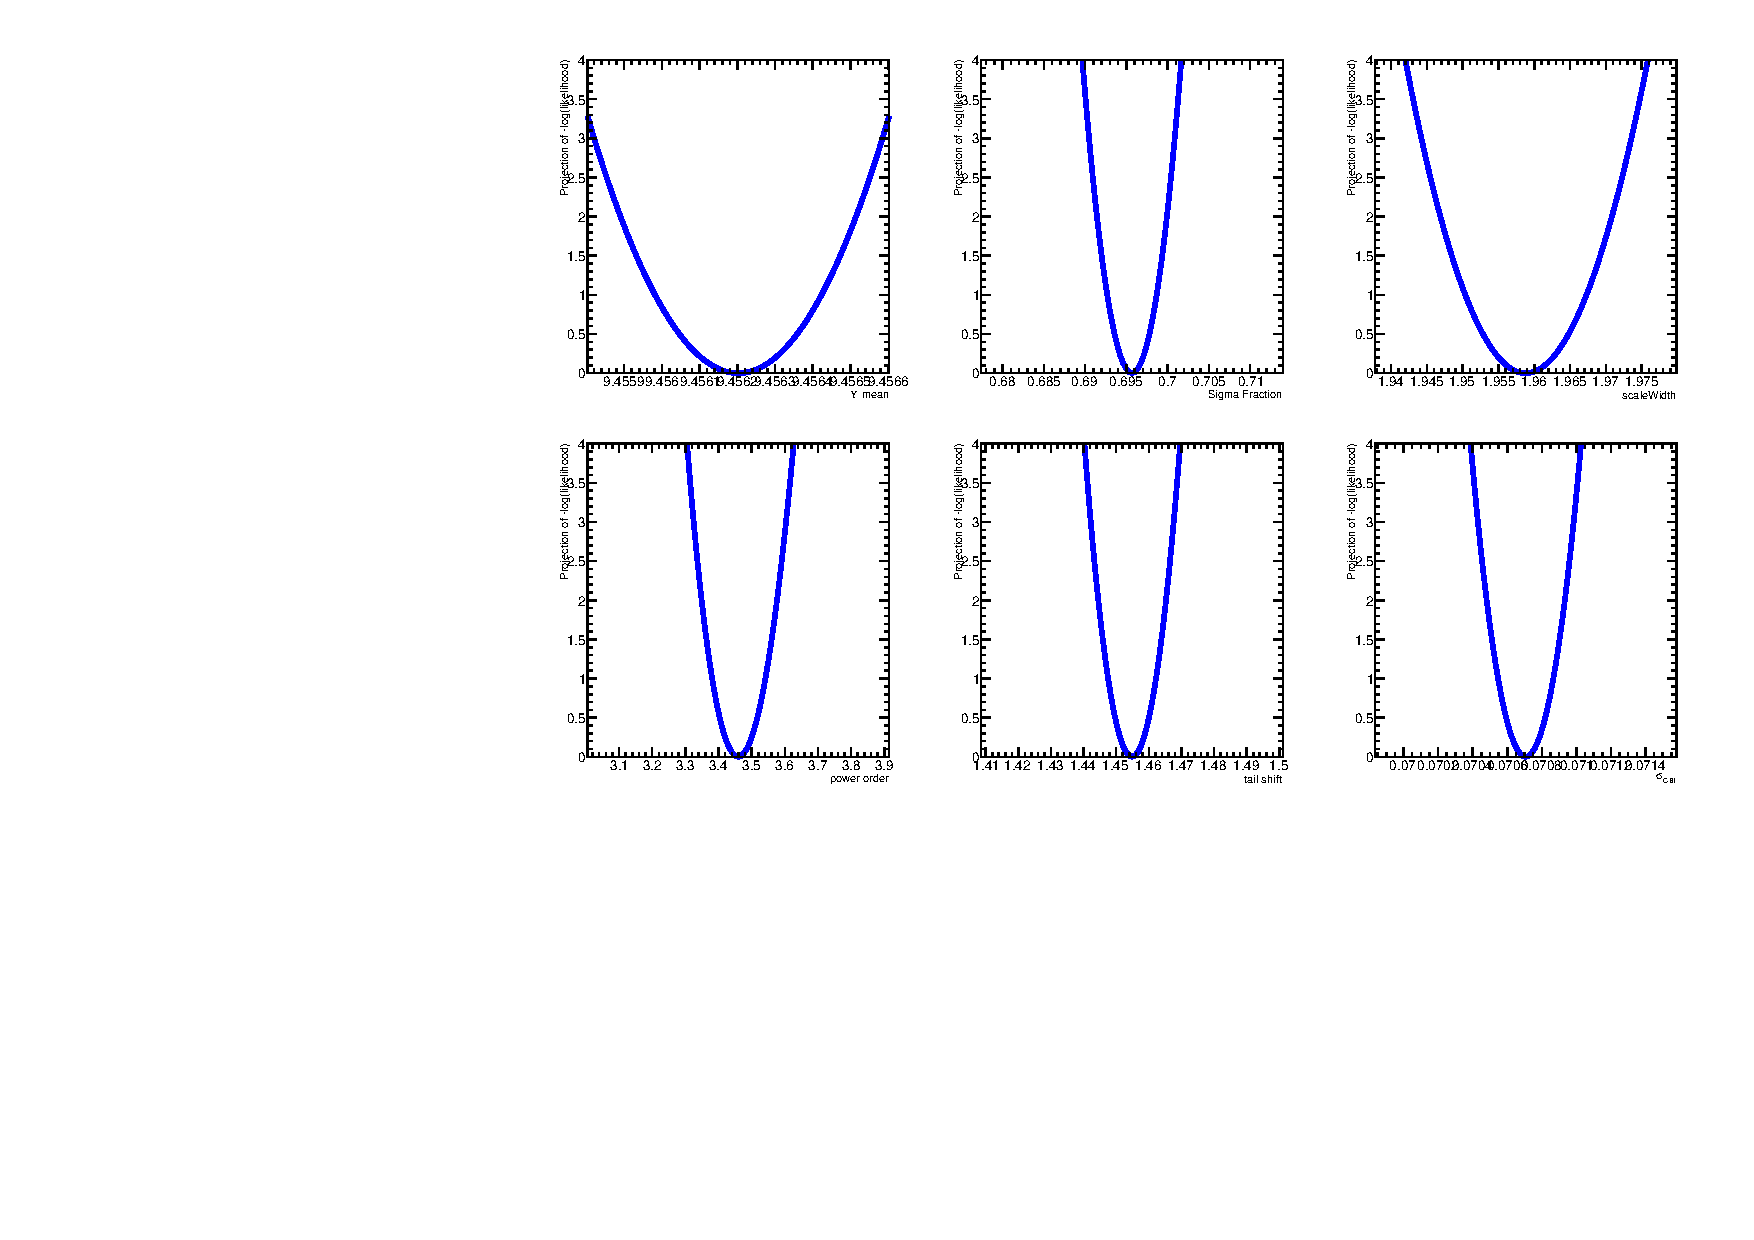
\includegraphics[width=1\textwidth]{Chapters/aYield/likelihoodScanExampleMinBias.pdf}  
\caption{A good likelihood scan of the all integrated $\Upsilon$(1S)
  sample.}
\label{fig:likelihoodScanExampleMinBias}
\end{center}
\end{figure}


The Table~\ref{tab:FSRparameters} in Appendix~\ref{sec:figs} provides the central
values obtained for each parameter in the signal shape. These
parameters are further used for signal fitting and systematics.

\subsection{Extraction of raw \texorpdfstring{\PgU}{Y} yields}
\label{sec:sigext_yield}

 Figures \ref{fig:yieldsNoPulls_pt3p5} and \ref{fig:yieldsNoPulls_pt4}
 show the fit to the full datasets extracted in both (pp and PbPb)
 data sets, with the
 signal-plus-background function $\F$. Figure~\ref{fig:yieldsNoPulls_pt3p5} presents results of the \PgUa\ analysis
selection (with loose muon $\pt$ cuts), while
Figure \ref{fig:yieldsNoPulls_pt4} presents results for the excited
states (tight muon $\pt$ cuts). Results are also reported in Table \ref{tab:MinBiasTable}.
%
\begin{figure}[h]
\centering
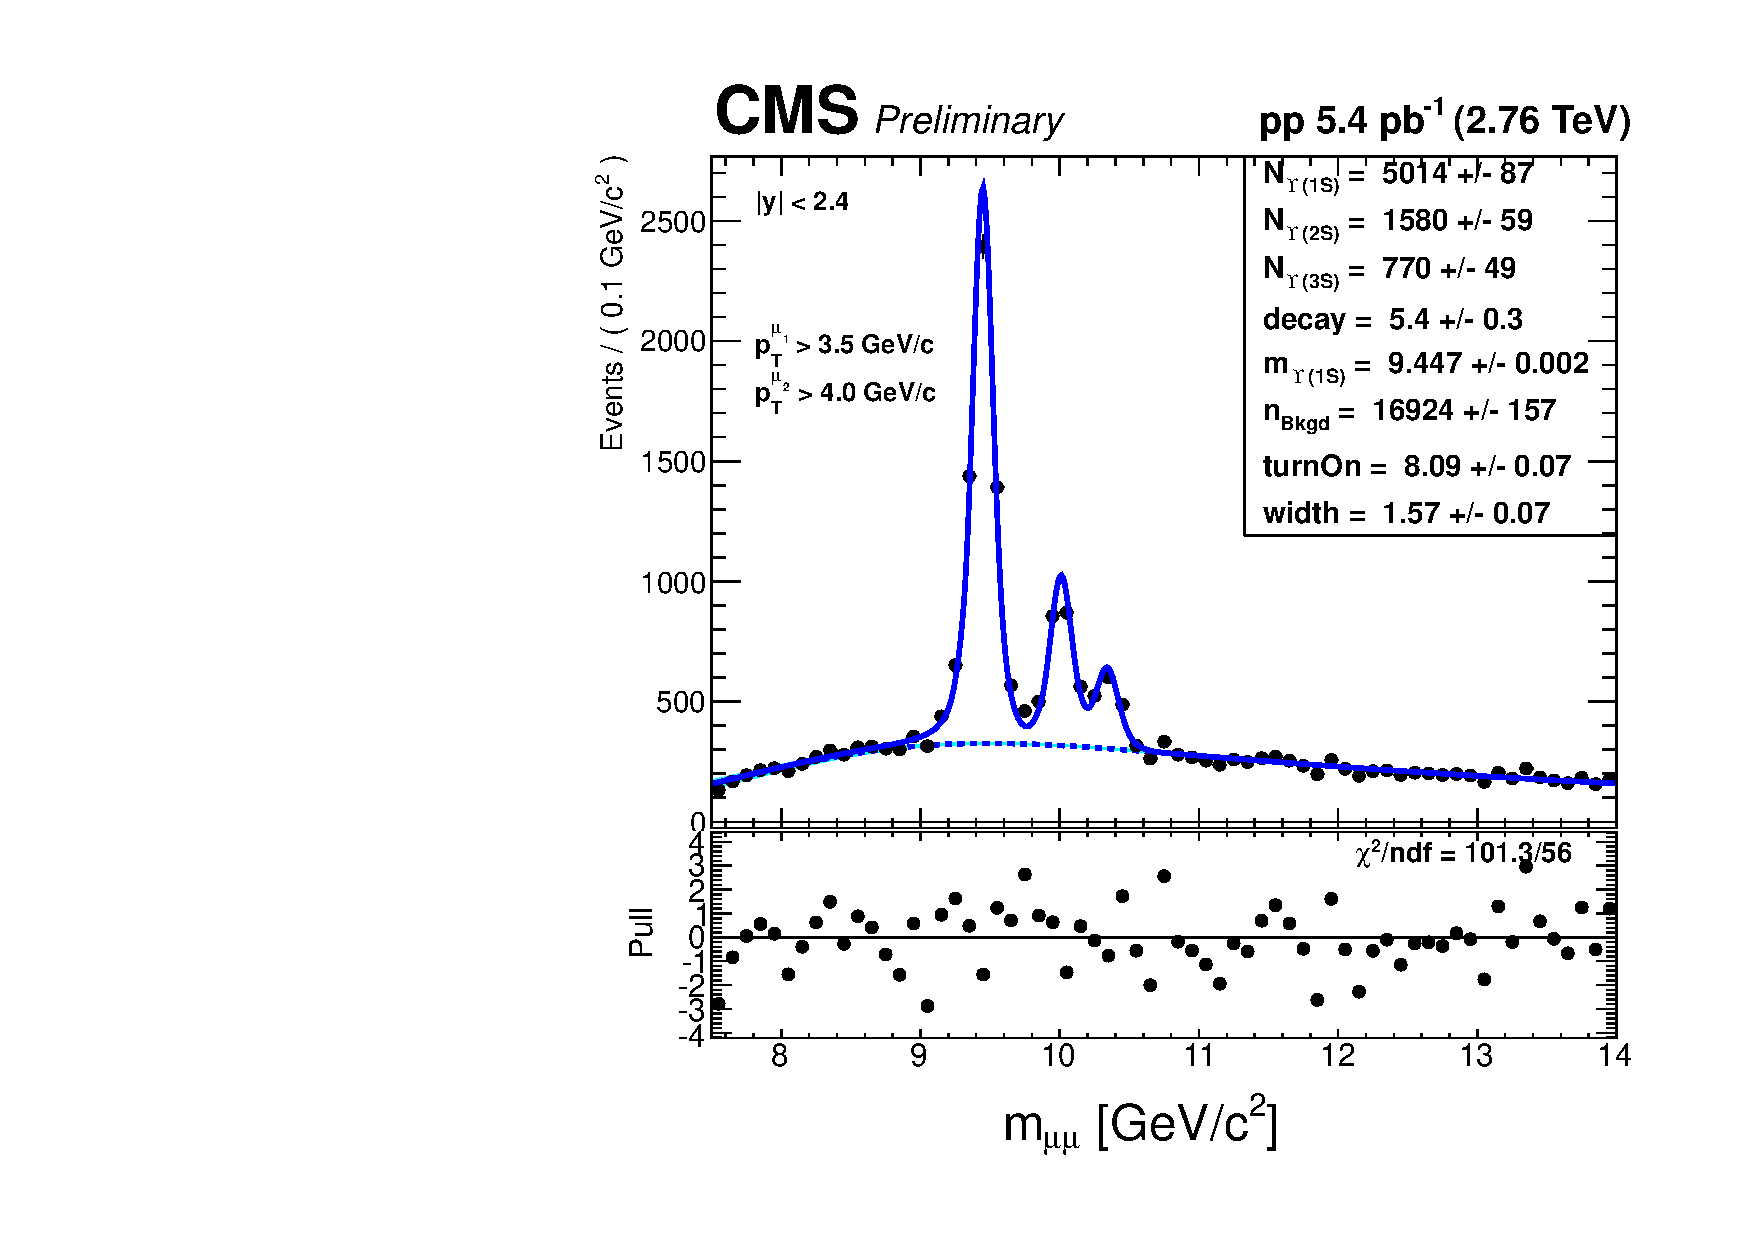
\includegraphics[width=0.49\textwidth]{Chapters/aYield/pp/pt_3p5_4/Rap/Rap_0_2p4/pp2p76tev_Rap_0_2p4_fsr1_3Spositive.pdf}
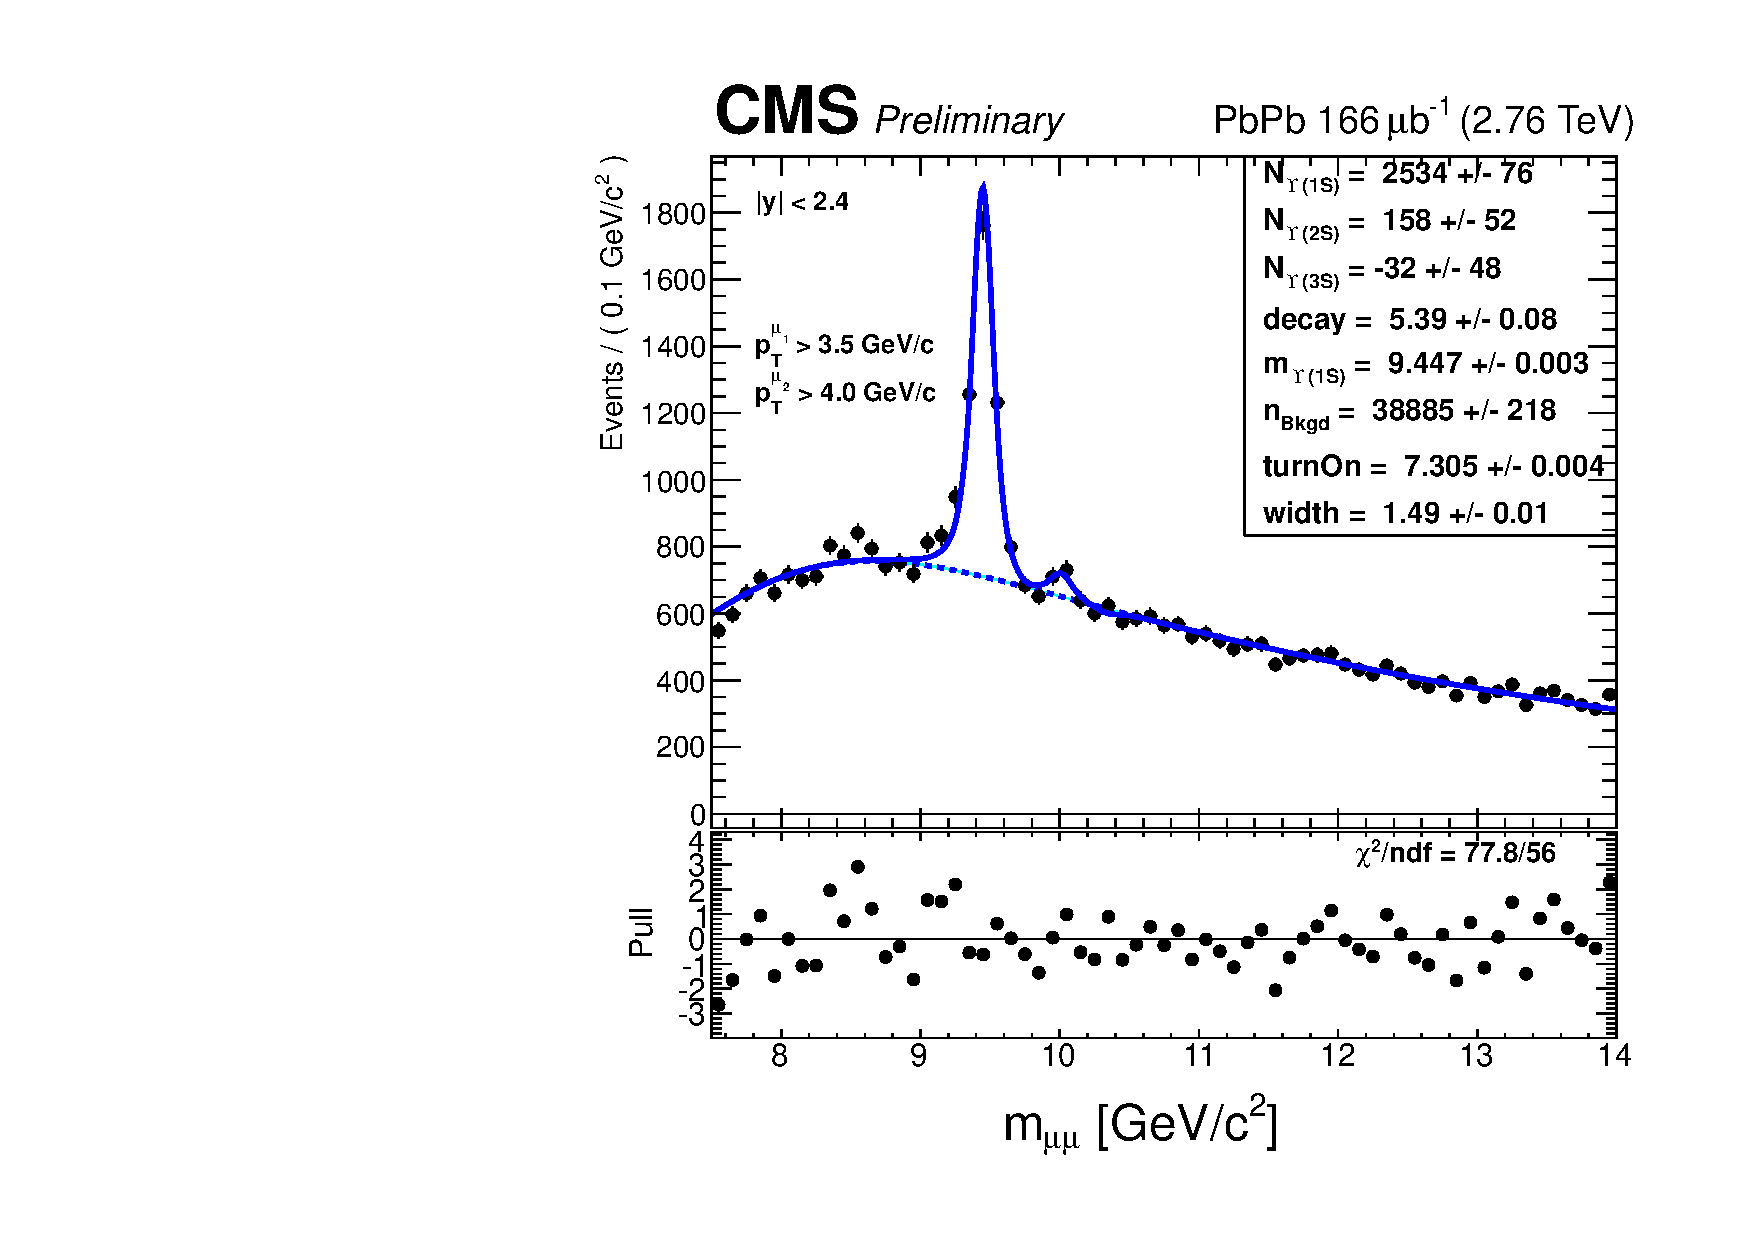
\includegraphics[width=0.49\textwidth]{Chapters/aYield/PbPb/pt_3p5_4/Rap/Rap_0_2p4/PbPb_Rap_0_2p4_fsr1.pdf}
\caption{\label{fig:yieldsNoPulls_pt3p5} Invariant-mass fits to all pp data (left) and PbPb data
  (right). The solid blue line is the total fit
  function, the background being the underlying dashed curve. The
  light blue band around the background shape is the 1$\sigma$ error
  band on background fitting.}
\end{figure}

\begin{figure}[h]
  \centering
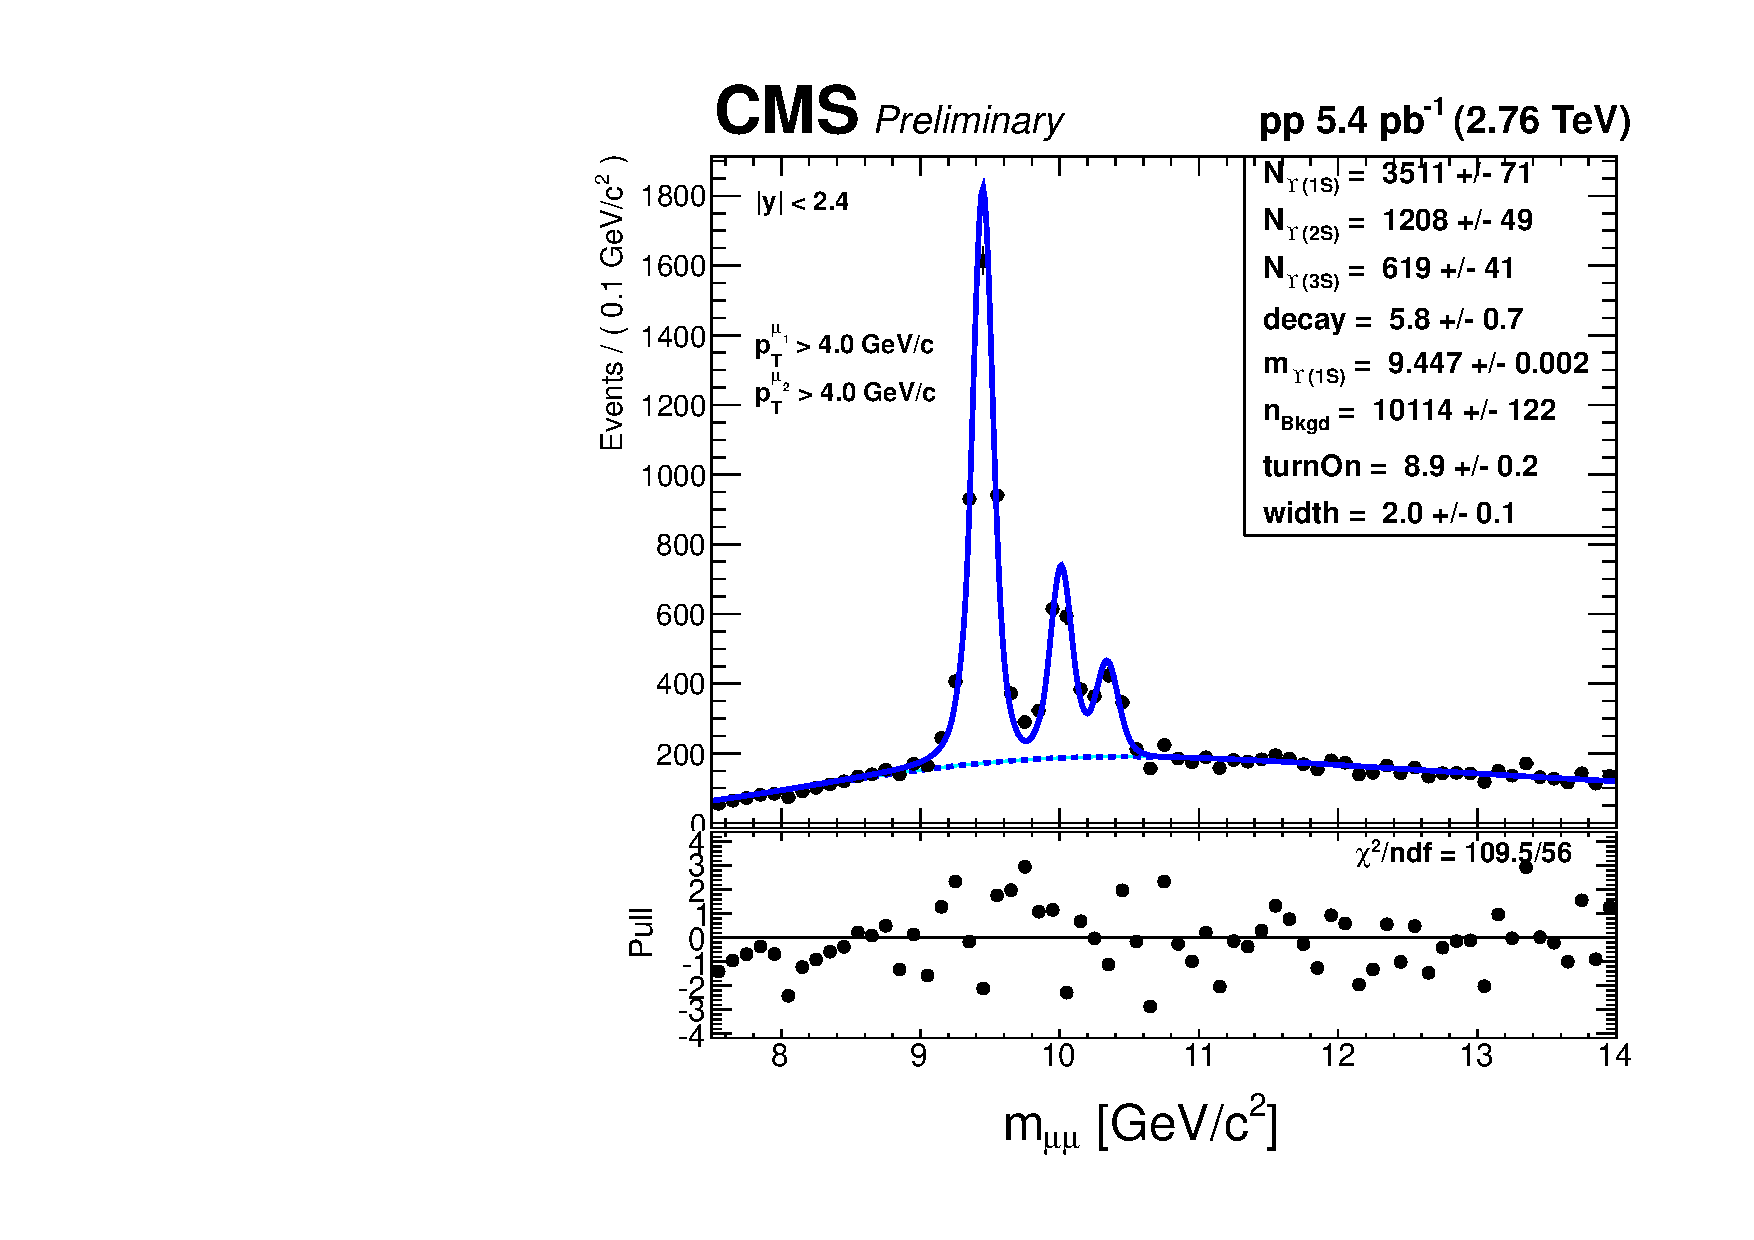
\includegraphics[width=0.49\textwidth]{Chapters/aYield/pp/pt_4_4/Rap/Rap_0_2p4/pp2p76tev_Rap_0_2p4_fsr1_3Spositive.pdf}
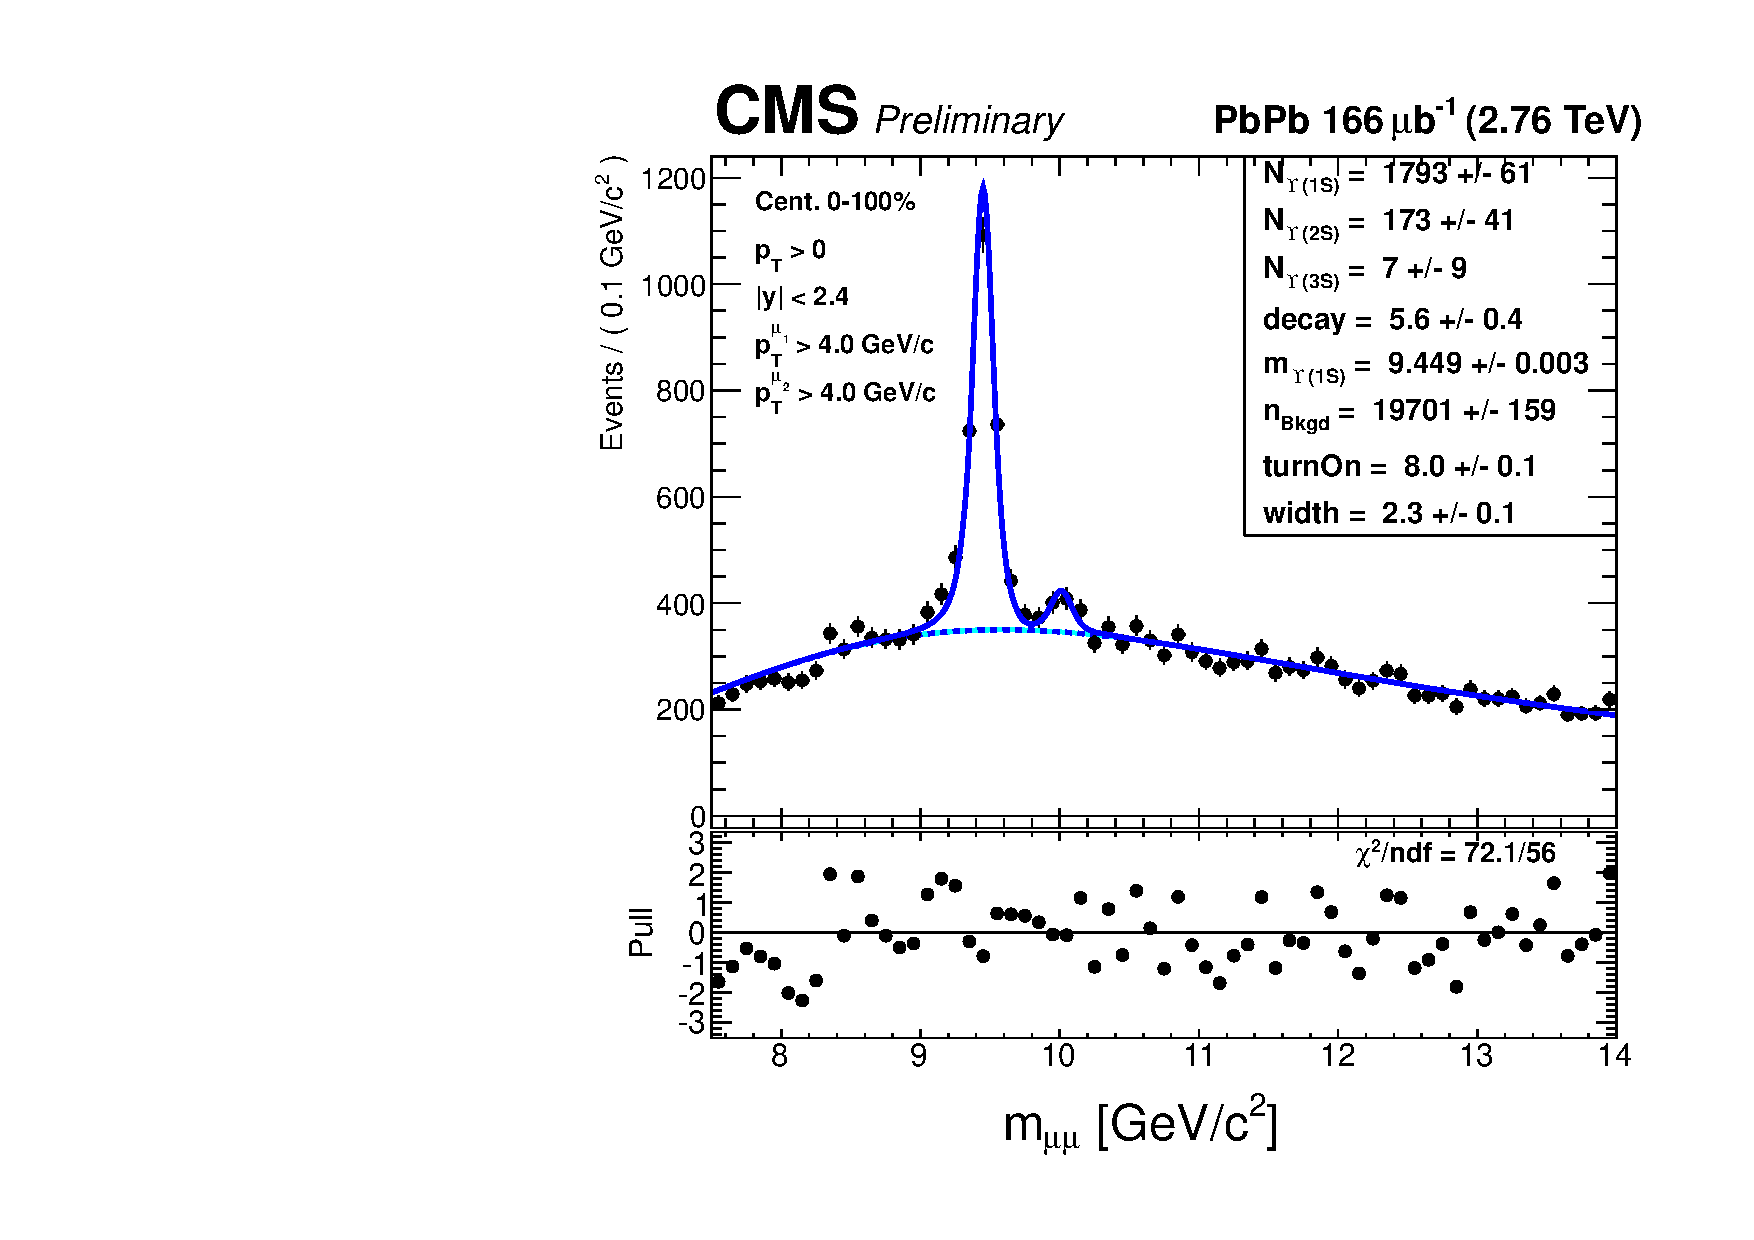
\includegraphics[width=0.49\textwidth]{Chapters/aYield/PbPb/pt_4_4/Centrality/Cent_0_100/PbPb_Cent_0_100_fsr1_3Spositive.pdf}
%  Invariant-mass fits to full PbPb data
%  (left) and pp data (right). This time, 
\caption{\label{fig:yieldsNoPulls_pt4} Same as Figure~\ref{fig:yieldsNoPulls_pt3p5} using tight muon \pt cuts. }
\end{figure}
%
%
\begin{table}[h]
  \centering
    \begin{tabular}{c|c|c|c}
%      $\pt^{\mu} >$ 3.5 OR 4 GeV/c 
      Loose cuts
      & $\NFitOneS$ & $\NFitTwoS$ & $\NFitThreeS$\\
      \hline
      PbPb &2534$\pm$76&158$\pm$52&-32$\pm$48  \\ 
      pp   &5014 $\pm$ 87 & 1580$\pm$59&770$\pm$49\\ 
      \hline \hline
      Tight cuts
       & $\NFitOneS$ & $\NFitTwoS$ & $\NFitThreeS$\\
      \hline
      PbPb &1793$\pm$61&173$\pm$ 41& 7$\pm$9  \\ 
      pp   &3511 $\pm$ 71& 1208$\pm$49&619$\pm$41\\ 
      \hline
    \end{tabular}

\caption{Table for fit results of the three \PgU\ states, when
  measured on the full $pp$ and PbPb samples.} 
\label{tab:MinBiasTable}
\end{table}


\subsubsection{Transverse momentum bins}
\label{binning}
\label{subsec:ptbins}
  For both the pp and PbPb analyses, the $\pt$ binning used is
  \begin{eqnarray}
  \PgUa:&& \pt~[{\rm GeV}/c] \in [0 - 2.5], [2.5 - 5], [5 - 8],[8 -  12], [12 - 20] \ ,\nonumber  \\
  \PgUb:&& \pt~[{\rm GeV}/c] \in [0 - 5], [5 - 12] \nonumber \ ,
\end{eqnarray}
for  $\PgUa$ and  
$\PgUb$, respectively. This binning has been chosen specifically to
obtain about the same number of candidates in most of the bins. % It is to be
% noted that the recorded statistics does not allow for the
% $\pt$ binning of $\PgUc$ states in PbPb.

The fits to data for $\PgUa$ (loose muon cuts) and $\PgUb$ (tight muon cuts) %(using respectively loose and tight muon selection cuts) 
are reported from in Appendix~\ref{sec:figs_pt}, Figures \ref{fig:YieldsErfExp_pt1Sa} to \ref{fig:YieldsErfExp_pt2Sb}.


\subsubsection{Rapidity binning}
\label{subsec:rapbins}
For both the pp and PbPb analyses, the  $y$ binning used is
%
 \begin{eqnarray}
  \PgUa:&& y \in [0 - 0.4], [0.4 - 0.8], [0.8 - 1.2], [1.2 - 1.6], [1.6 - 2], [2 - 2.4] \ ,
  \nonumber  \\
    \PgUb:&& y \in [0 - 1.2], [1.2 - 2.4] \nonumber \ ,
\end{eqnarray}
for \PgUa\ and \PgUb. %
% The $y$ binning in the  $\PgUb$ channel corresponds to the
% one used in 2010 in~\cite{Chatrchyan:2012np} for the kinematics of $\PgUa$.
%
% The too limited statistics does not allow for the $y$ binning of $\PgUc$ states.

The fits to data for $\PgUa$ and $\PgUb$ analyses are reported
in Appendix~\ref{sec:figs_y}, from Figures~\ref{fig:YieldsErfExp_y1Sa} to \ref{fig:YieldsErfExp_y2Sb}, respectively. 


% 
%
\vfill\newpage
\subsubsection{Centrality dependence}
\label{subsec:centbins}
% Fig.\ref{fig:YieldsErfExp_aapt1S} sums up the nominal fits
% performed on PbPb data with the $\pt$ binning described above, for
% extraction of the $\PgUa$ yields.
The study of the centrality dependence is performed separately for  $\PgUa$ and $\PgUb$ states.% using the same centrality classes as in~\cite{an_hin-11-011}.
% The
%yields for $\PgUa$ are again extracted with the use of a loose muon
%p$_{T} > $ 3.5 or 4 GeV cut, and the $\PgUb$ are extracted
%applying a tighter cut, p$_{T} > $ 4 GeV.
The centrality binning used in PbPb is:

\begin{eqnarray}
  &\PgUa&\textrm{Cent. }\in [0-5], [5-10], [10-20], [20-30],
  [30-40], [40-50], [50-70], [70-100] \% \nonumber  \\
  &\PgUb&\textrm{Cent. }\in [0-10], [10-30], [30-50], [50-100] \% \nonumber ,
\end{eqnarray}

The fits to data for the $\PgUa$ analysis are reported
in Appendix~\ref{sec:figs_cent}, Figures~\ref{fig:YieldsCent1S} and~\ref{fig:YieldsCent1SContd}. For
the \PgUb, the PbPb yields were too low to bin in centrality with a
binning as fine as \PgUa. The 2011 analysis~\cite{11-011} reported
\PgUb\ yields in small bins equivalent to those of the \PgUa\
analysis, however most of them yielded results compatible with
zero. In order to avoid poorly significant results where one cannot
tell if the observed measurement are due to statistical fluctuations, the centrality
bins have been reduced to four in the present analysis. Yields for the $\PgUb$ analysis are
extracted from the fits reported in Figure~\ref{fig:YieldsCent2S}.

%\vfill\newpage

\subsection{Systematic uncertainties from signal extraction}
\label{sec:sigext_vars}

As mentioned in Section~\ref{sec:sigext_fits},
variations are performed upon the nominal fit function in order to compute the systematic
uncertainty from the fitting method. The uncertainty from fitting is computed
as the quadratic sum of two sources: varying the signal lineshape by releasing
constraints on the signal parameters, and varying the PDF used for the
background continuum. The variations on the signal $\Sig$ and
background $\B$ are described below and were performed
independently for each analysis bin and muon \pt\ cut:\\ ~\\
\noindent {\bf Signal shape variation}
\begin{itemize}
%\item{Releasing \textit{all} signal shape parameters;}
\item {To test the hypothesis that fit parameters could be poorly
    reproduced by the MC simulations, all the 5 parameters ($n, \alpha, \sigma_{0}, f, x$)
  released one by one in the fit to the data (the other 4 being fixed
  to their constrained MC value), leading to 5 fits per bin. For the signal, the
  systematic uncertainty is taken to be the RMS of the five variations to the nominal
  fit in a given bin.}
\end{itemize}
{\bf Background shape variation}
\begin{itemize}
%\item{Releasing $f$ the normalisation fraction of CB$_{1}$ and CB$_{2}$
  %  in the double Crystal Ball function;}
\item{To estimate the signal systematic uncertainty coming
    from our description of the background continuum below the peak, variations
    on the background PDF are performed. The default background shape $\B$ receives an additional (unconstrained) first order Chebychev polynomial}
\item{Same operation, with a second order Chebychev polynomial. The uncertainty
  from background is computed as the maximum of the two
  deviations to the nominal fit.}
\end{itemize}

In Appendix~\ref{sec:figs_syst}, Figure~\ref{fig:fitVar_ppMB-1}, the fit variations of the $pp$
all-integrated sample are reported, and continued onto
Figure~\ref{fig:fitVar_ppMB-2}. 


In Appendix~\ref{sec:figs_syst}, Figure~\ref{fig:fitVar_AAMB-1}, the fit variations of the PbPb
all-integrated sample are reported, and continued onto Figure~\ref{fig:fitVar_AAMB-2}.


In the following Tables \ref{tab:systrecap1},~\ref{tab:systrecap2},~\ref{tab:systrecap3}, the systematic
uncertainties computed for each bin are reported for \PgUa\ (pp and PbPb),
\PgUb\ and \PgUc\ pp, and \PgUb\ PbPb analyses respectively. Namely, the relative deviations are shown for each fit in
every bin. The total systematic
uncertainty per bin is derived in the last column (quadratic sum of
total signal and total background uncertainties).


%\vfill\newpage 
\begin{table}[h]
\begin{centering}
\begin{tabular}{c|c|c|c|c|c|c|c||c}
 & \multicolumn{5}{c}{Signal} \vline & \multicolumn{2}{c}{Background}
 \vline& Total \%\\
\hline
$pp$ \PgUa\ &$\alpha$ & $n_{CB}$ & $\sigma_{1}$ &
$\sigma_{2}/\sigma_{1}$ & $f$ & Pol(1)&Pol(2)& Tot. pp\%\\
\hline
\pt\ $<$ 2.5 & 4.41 & 3.71 & -9.21 & -9.33 & -7.38 & 0.13 & -2.51 & 8 \%\\
2.5 $<$ \pt\ $<$ 5 & 4.55 & 3.86 & -1.98 & -1.05 & -1.92 & 0.19 & -4.07 & 5 \%\\
5 $<$ \pt\ $<$ 8 & -2.26 & -7.44 & -2.12 & -2.17 & -1.59 & 0.47 & 0.89 & 4 \%\\
8 $<$ \pt\ $<$ 12 & -1.84 & 0.25 & -2.90 & -2.71 & -2.33 & -0.02 & -0.72 & 2 \%\\
12 $<$ \pt\ $<$ 20 & -0.07 & -0.94 & -1.04 & -0.55 & -1.01 & 0.00 & 0.00 & 1 \%\\
%20 $<$ \pt\ $<$ 40 & -5.94 & -8.88 & -5.18 & -7.97 & -1.47 & -0.01 & -1.43 & 7 \%\\
\hline
$|y| <$ 0.4 & -5.02 & -2.14 & -1.79 & -1.34 & -0.01 & 1.08 & 1.38 & 3\%\\
0.4 $< |y| <$ 0.8   & -1.54 & -2.24 & -2.61 & -3.50 & -2.70 & 0.78 & -0.13 & 3\%\\
0.8 $< |y| <$ 1.2  & -2.62 & -4.35 & -1.31 & -0.50 & -1.17 & 2.96 & 2.99 & 4\%\\
1.2 $< |y| <$ 1.6  & -1.71 & 3.54 & -3.99 & -6.00 & -2.66 & 1.93 & -0.13 & 4\%\\
1.6 $< |y| <$ 2    & 3.07 & 1.99 & -7.52 & -7.71 & -0.01 & 1.21 & 0.31 & 5\%\\
2 $< |y| <$ 2.4    & 1.35 & -2.38 & 2.63 & 3.90 & 2.98 & -7.73 & -0.53 & 8\%\\
\hline
 PbPb \PgUa\ &$\alpha$ & $n_{CB}$ & $\sigma_{1}$ &
$\sigma_{2}/\sigma_{1}$ & $f$ & Pol(1)&Pol(2)& Tot. PbPb\%\\
\hline
\pt\ $<$ 2.5 & -15.18 & -4.45 & -5.95 & -10.07 & -4.66 & 0.03 & 0.69 & 9 \%\\
2.5 $<$ \pt\ $<$ 5 & -6.47 & -0.84 & -7.45 & -6.24 & -6.91 & -0.00 & -2.16 & 6 \%\\
5 $<$ \pt\ $<$ 8 & -17.25 & -22.27 & 5.45 & -9.37 & 3.27 & -0.62 & -2.38 &12 \%\\
8 $<$ \pt\ $<$ 12 & 5.28 & 1.60 & -5.25 & -1.84 & -5.46 & -0.35 & -0.13 & 4 \%\\
12 $<$ \pt\ $<$ 20 & -0.73 & 0.72 & 0.05 & -0.60 & -0.47 & -3.78 & -2.00 & 4 \%\\
%20 $<$ \pt\ $<$ 40 & -0.34 & 0.54 & 0.29 & 2.12 & 0.83 & 59.81 & -4.59 & 5 \%\\
\hline
$|y| <$ 0.4 & -11.11 & -4.38 & -0.63 & 0.37 & -1.00 & 0.01 & 0.97 & 5\%\\
0.4 $< |y| <$ 0.8   & -23.66 & -4.96 & -0.50 & 0.45 & -0.73 & 1.74 & -1.94 & 11\%\\
0.8 $< |y| <$ 1.2  & -17.01 & -4.45 & -1.50 & -8.49 & -0.76 & -5.66 & -15.15 & 18\%\\
1.2 $< |y| <$ 1.6  & 5.05 & 4.37 & -6.06 & 0.90 & -8.69 & -4.65 & 7.47 & 9\%\\
1.6 $< |y| <$ 2    & -21.47 & -10.51 & -1.60 & -0.82 & -5.33 & 0.01 & -18.56 & 22\%\\
2 $< |y| <$ 2.4    & -43.54 & -13.35 & -14.46 & -10.82 & -12.77 & -16.58 & -15.77 & 28\%\\
\hline
0-5 & 8.307 & -18.687 & 13.935 & 12.136 & 12.161 & -16.809 & -0.002 & 14.4\%\\
5-10 & -1.265 & 3.440 & -4.991 & -1.337 & -5.477 & 1.652 & -3.915 & 12.0\%\\
10-20 & -24.197 & -20.448 & -8.347 & -8.713 & -6.883 & 4.301 & -2.396 & 10.3\%\\
20-30 & -12.225 & -19.523 & -8.183 & -7.417 & -7.562 & 0.770 & 1.073 & 8.5\%\\
30-40 & 1.041 & 1.333 & 0.893 & 1.038 & 0.655 & -0.036 & -8.471 & 12.0\%\\
40-50 & -5.149 & -19.713 & -3.219 & -9.837 & -1.663 & 0.332 & -0.417 & 15.7\%\\
50-70 & -19.041 & -16.327 & -5.668 & -2.435 & -5.488 & -1.896 & 2.248 & 5.4\%\\
70-100 & -25.068 & -20.123 & -0.930 & -1.582 & -1.285 & 0.152 & 0.209 & 21.5\%\\
\hline
\end{tabular}
\caption{Systematic deviations from the central result for \PgUa\ fitting
  in pp and PbPb, reported for
  each analysis bin. Last column: total systematic uncertainty from
  fitting.}
\label{tab:systrecap1}
\end{centering}
\end{table}
\vfill
\begin{table}[h]
\begin{centering}
\begin{tabular}{c|c|c|c|c|c|c|c||c}
 & \multicolumn{5}{c}{Signal} \vline & \multicolumn{2}{c}{Background}
 \vline& Total \%\\
\hline
$pp$ \PgUb\ &$\alpha$ & $n_{CB}$ & $\sigma_{1}$ &
$\sigma_{2}/\sigma_{1}$ & $f$ & Pol(1)&Pol(2)& Tot. \PgUb\\%\\
\hline

\pt\ $<$ 2.5 & 4.78 & 3.07 & -3.00 & 0.49 & -2.83 & 0.38 & -10.60 &11 \%\\
2.5 $<$ \pt\ $<$ 5 & 5.33 & 4.37 & -0.34 & 0.66 & -1.15 & 0.02 & -3.05 &4 \%\\
5 $<$ \pt\ $<$ 8 & -5.32 & -3.79 & -3.71 & -3.10 & -2.97 & 1.47 & -1.54 &4 \%\\
8 $<$ \pt\ $<$ 12 & -3.84 & -1.00 & -3.92 & -2.84 & -3.49 & -0.13 & -0.45 &3 \%\\
12 $<$ \pt\ $<$ 20 & 0.53 & 0.81 & -0.24 & 0.15 & -0.15 & 0.37 & 0.87 &1 \%\\
%20 $<$ \pt\ $<$ 40 & -10.73 & -13.63 & -3.86 & -6.97 & -1.09 & -4.73 & 0.85 &0.10 \%\\
\hline
$|y| <$ 0.4 & -1.74 & 2.54 & -4.58 & -5.21 & -0.47 & 4.70 & 3.10 & 5\%\\
0.4 $< |y| <$ 0.8   & -4.13 & 0.17 & -4.95 & -6.58 & -4.35 & -0.00 & -2.36 & 5\%\\
0.8 $< |y| <$ 1.2  & -4.22 & -6.56 & -3.63 & -3.49 & -3.41 & 9.57 & -7.66 & 9\%\\
1.2 $< |y| <$ 1.6  & 0.85 & 3.80 & -5.48 & -6.60 & -3.90 & 0.74 & 7.55 & 9\%\\
1.6 $< |y| <$ 2    & -7.15 & 2.34 & -8.97 & -8.65 & -1.81 & -0.26 & 12.26 & 14\%\\
2 $< |y| <$ 2.4    & 3.59 & -3.08 & -0.13 & 0.03 & 0.08 & 0.02 & 1.85 & 3\%\\
\hline

 $pp$ \PgUc\ &$\alpha$ & $n_{CB}$ & $\sigma_{1}$ &
$\sigma_{2}/\sigma_{1}$ & $f$ & Pol(1)&Erf$\cdot$exp +
Pol(2)& Tot. 3S\%\\
\hline
\pt\ $<$ 2.5 & 7.10 & 4.28 & -3.95 & 0.55 & -3.77 & 0.49 & -14.40 & 15 \%\\
2.5 $<$ \pt\ $<$ 5 & 6.67 & 5.44 & -0.35 & 0.52 & -1.05 & 0.01 & -3.09 &5 \%\\
5 $<$ \pt\ $<$ 8 & -8.12 & -5.05 & -3.95 & -2.01 & -2.92 & -0.28 & -1.67 &5 \%\\
8 $<$ \pt\ $<$ 12 & -6.56 & -1.37 & -3.50 & -1.22 & -3.36 & -0.20 & -0.93 &4 \%\\
12 $<$ \pt\ $<$ 20 & 1.11 & 1.13 & -0.25 & 0.10 & -0.15 & 0.78 & 1.75 &2 \%\\
%20 $<$ \pt\ $<$ 40 & -13.63 & -16.35 & -2.69 & -3.00 & -0.94 & -3.57 & 0.37 & 10 \%\\
\hline              							    
$|y| <$ 0.4 & -2.40 & 3.45 & -6.10 & -6.78 & -0.86 & 6.43 & 5.79 & 7\%\\
0.4 $< |y| <$ 0.8   & -6.64 & 0.24 & -8.26 & -8.06 & -6.87 & -0.02 & 1.19 & 7\%\\
0.8 $< |y| <$ 1.2  & -5.79 & -8.00 & -3.45 & -2.64 & -2.98 & 9.40 & -10.04 & 0.11\%\\
1.2 $< |y| <$ 1.6  & 1.27 & 5.73 & -5.01 & -5.96 & -3.72 & -2.00 & 9.35 & 0.10\%\\
1.6 $< |y| <$ 2    & -11.39 & 3.97 & -2.92 & -2.88 & 0.08 & -0.85 & 1.38 & 6\%\\
2 $< |y| <$ 2.4    & 4.14 & -3.17 & -0.13 & -0.13 & -0.15 & 0.05 & 1.01 & 3\%\\
\hline

\end{tabular}
\caption{Systematic deviations from the central result for \PgUb\ and \PgUc\ 
  fitting in pp, reported for
  each analysis bin. Last column: total systematic uncertainty from
  fitting.}
\label{tab:systrecap2}
\end{centering}
\end{table}


\begin{table}[h]
\begin{centering}
\begin{tabular}{c|c|c|c|c|c|c|c||c}
 & \multicolumn{5}{c}{Signal} \vline & \multicolumn{2}{c}{Background}
 \vline& Total \%\\
\hline
PbPb \PgUb\ &$\alpha$ & $n_{CB}$ & $\sigma_{1}$ &
$\sigma_{2}/\sigma_{1}$ & $f$ & Pol(1)&Pol(2)& Tot. \PgUb\\%\\
\hline
\pt\ $<$ 5         & -12.70 & -34.76 & -9.03 & -0.88 & -8.64 & 11.6 & 0.16 & 17 \%\\
5 $<$ \pt\ $<$ 12  & -9.70  & -15.42 & -2.51 & -6.93 & -4.89 & -1.3 & -7.20 & 12 \%\\
12 $<$ \pt\ $<$ 40 & -1.39  & -1.57  & -0.17 & -0.50 & -0.29 & -11.8& -9.72 & 12 \%\\    
\hline
$|y| <$ 1.2  & -13.42 & -17.01 & -3.21 & -7.89 & -2.38 & 6.56 & 27.51 & 29 \%\\
1.2 $< |y| <$ 2.4    & -66.45 & -13.63 & -16.73 & -0.20 & -0.01 & 8.12 & 41.92 & 52 \%\\
\hline
\hline
0-10    & -54.2 & -44.1 & -19.0 & -11.4 & -18.8 & 21.8 & 28.0 & 45\%\\
10-30   & -21.8 & -34.2 & -19.3 & -14.3 & -15.5 & 28.2 & -12.3 & 56\%\\
30-50   & -34.7 & -55.3 & -26.8 & -24.4 & -17.4 & 70.8 & 44.2 & 25\%\\
50-100  & -81.6 & -46.7 & -6.5 & -11.6  & -5.5 & -12.4 & -16.9 & 44\%\\
\hline
\end{tabular}
\caption{Systematic deviations from the central result for \PgUb\ 
  fitting in PbPb, reported for
  each analysis bin. Last column: total systematic uncertainty from
  fitting.}
\label{tab:systrecap3}
\end{centering}
\end{table}
\newpage 

\subsection{Tabulated results}
This Section sums up the fit results of each analysis. The
paragraph is organised as follows:
Table~\ref{tab:YieldsLoose} reports the results on raw yields for the extraction
of $\PgUa$ cross-section and \RAA\ differential in rapidity
or transverse momentum. As a reminder, let me mention here the \PgUa\
analysis is performed with what was earlier called 'loose' single muon
\pt\  cuts. For completeness, the yields of excited states from
these \PgUa\ fits are also reported, but do not enter in the computation of
excited states cross sections or \RAA. 

Table~\ref{tab:YieldsTight} reports the results on raw yields for the extraction
of yields with the 'tight' single muon \pt\  cut. This cut is
applied to the $\Upsilon$(2S,3S) pp cross section and \RAA. Since
the available statistics is large in pp, the results for pp cross
sections are taken from
small bins (lower panel). The PbPb yields are tabulated for both binning formats,
and the \RAA results are taken from large bins (upper panel).

Table \ref{tab:YieldsCentrality} reports the results on raw yields in
bins of centrality. The upper panel consists of yields used in the \PgUa\
\RAA\ analysis, extracted with loose muon \pt\  cuts, while the
lower panel consists of yields extracted with p$^{\mu}_{T} >$ 4 \GeVc,
for the \PgUb\ \RAA. The \PgUa\ yields from the lower panel can be used to
compare with 2011 results, and feature an overall 35 percent signal
increase attributed to the improved reconstruction (RegIT).

% \vfill\newpage

\begin{table}[hbtp]
  \begin{centering}
    \begin{tabular}{c|c|c|c|c|c}
      \hline
      Fit Results &  \multicolumn{3}{c}{pp} \vline& \multicolumn{2}{c}{PbPb}  \\                                               
      \hline
      % p$_{T}^{\mu} <$ (3.5 or 4) GeV
      Loose cuts & $\NFitOneS$ & $\NFitTwoS$ & $\NFitThreeS$  &  $\NFitOneS$ &  $\NFitTwoS$ \\  
      \hline                                                                                                   
      $\pt <$ 2.5 & \textbf{1572 $\pm$ 53} &  413 $\pm$ 34 &  190 $\pm$ 28 & \textbf{761 $\pm$ 43} & 39 $\pm$ 28 \\  
      2.5 $< \pt <$ 5 & \textbf{1440 $\pm$ 46} & 498 $\pm$ 33 &  266 $\pm$ 28 & \textbf{679 $\pm$ 42} & 61 $\pm$ 30  \\  
      5 $< \pt <$ 8 &\textbf{ 992 $\pm$ 34} &  330 $\pm$ 22 &  150 $\pm$ 17 & \textbf{531 $\pm$ 34} & 23 $\pm$ 24  \\  
      8 $< \pt <$ 12 &\textbf{ 613 $\pm$ 28} &  226 $\pm$ 19 &  108 $\pm$ 15 & \textbf{362 $\pm$ 27} & 33 $\pm$ 19  \\  
      12 $< \pt <$ 20 & \textbf{338 $\pm$ 20} &  129 $\pm$ 14 &  76 $\pm$ 11 & \textbf{178 $\pm$ 16} & 21 $\pm$ 9  \\  
      \hline
      $|y| <$ 0.4 & \textbf{1092 $\pm$ 38} &  354 $\pm$ 25 &  165 $\pm$ 20 & \textbf{502 $\pm$ 32} & 26 $\pm$ 21 \\  
      0.4 $< |y| <$ 0.8 & \textbf{1129 $\pm$ 40} &  344 $\pm$ 26 &  171 $\pm$ 21 & \textbf{505 $\pm$ 34} & 48 $\pm$ 25  \\  
      0.8 $< |y| <$ 1.2 &\textbf{ 996 $\pm$ 39} &  314 $\pm$ 27 &  170 $\pm$ 23 & \textbf{559 $\pm$ 38} & 25 $\pm$ 27  \\  
      1.2 $< |y| <$ 1.6 & \textbf{919 $\pm$ 38} &  320 $\pm$ 28 &  123 $\pm$ 23 & \textbf{533 $\pm$ 39} & -1 $\pm$ 28  \\  
      1.6 $< |y| <$ 2 & \textbf{645 $\pm$ 34} &  215 $\pm$ 24 &  86 $\pm$ 20 & \textbf{365 $\pm$ 29} & 34 $\pm$ 19  \\  
      2 $< |y| <$ 2.4 &\textbf{ 251 $\pm$ 20} &  49 $\pm$ 13 &  56 $\pm$ 12 & \textbf{114 $\pm$ 17} & 4 $\pm$ 11  \\  
      \hline
    \end{tabular}
    \caption{Fit results of signal parameters using the loose cuts
      ($\PgUa$ analysis). The values actually used in the cross
      section computation are displayed with a bold font. Even if only
      the values fitted for the \PgUa\ peak will be used further, the
      fit results of \PgUb\ and \PgUc\ are also reported. The fit
      results follow the yields reported in
      Figures~\ref{fig:YieldsErfExp_pt1Sa},~\ref{fig:YieldsErfExp_pt1Sb},
      ~\ref{fig:YieldsErfExp_pt1Sc}~\ref{fig:YieldsErfExp_pt1Sd} and
      ~\ref{fig:YieldsErfExp_pt1Se}.}
    \label{tab:YieldsLoose}
  \end{centering}
\end{table}



\begin{table}[hbtp]
  \begin{centering}
    \begin{tabular}{c|c|c|c|c|c}
      \hline
      Fit Results &  \multicolumn{3}{c}{pp} \vline& \multicolumn{2}{c}{PbPb}  \\                                               
      \hline
      % p$_{T}^{\mu} <$ 4 GeV 
      Tight cuts & $\NFitOneS$ & $\NFitTwoS$ & $\NFitThreeS$  &  $\NFitOneS$ &  $\NFitTwoS$ \\  
      \hline 
      $\pt <$ 5 & 1815 $\pm$ 53 &  \textbf{562 $\pm$ 37} &  291 $\pm$ 33 & 846 $\pm$ 44 & \textbf{54 $\pm$ 31} \\  
      5 $< \pt <$ 12 & 1253 $\pm$ 40 & \textbf{ 446 $\pm$ 27} &  206 $\pm$ 22 & 660 $\pm$ 37 & \textbf{45 $\pm$ 24}  \\  
      12 $< \pt <$ 20 & 307 $\pm$ 19 &  \textbf{119 $\pm$ 13} &  69 $\pm$ 11 & 160 $\pm$ 15 & \textbf{22 $\pm$ 9}  \\  
      \hline
      $|y| <$ 1.2 & 2298 $\pm$ 55 & \textbf{ 769 $\pm$ 37} &  397 $\pm$ 31 & 1090 $\pm$ 46 & \textbf{104 $\pm$ 31} \\  
      1.2 $< |y| <$ 2.4 & 1213 $\pm$ 43 &  \textbf{451 $\pm$ 31} &  222 $\pm$ 26 & 729 $\pm$ 40 & \textbf{77 $\pm$ 27}  \\  


      \hline
      $\pt <$ 2.5 & 967 $\pm$ 40 &  \textbf{299 $\pm$ 29} &  \textbf{131 $\pm$ 24} & 433 $\pm$ 34 & 49 $\pm$ 24 \\  
      2.5 $< \pt <$ 5 & 802 $\pm$ 35 &  \textbf{254 $\pm$ 24} & \textbf{ 166 $\pm$ 22} & 385 $\pm$ 30 & 29 $\pm$ 21  \\  
      5 $< \pt <$ 8 & 722 $\pm$ 31 &  \textbf{246 $\pm$ 20} & \textbf{ 113 $\pm$ 16} & 346 $\pm$ 27 & 8 $\pm$ 18  \\  
      8 $< \pt <$ 12 & 524 $\pm$ 26 & \textbf{ 197 $\pm$ 18} & \textbf{ 90 $\pm$ 14} & 300 $\pm$ 25 & 29 $\pm$ 18  \\  
      12 $< \pt <$ 20 & 307 $\pm$ 19 & \textbf{ 119 $\pm$ 13} &  \textbf{69 $\pm$ 11} & 160 $\pm$ 15 & 22 $\pm$ 9  \\  
      \hline
      $|y| <$ 0.4 & 782 $\pm$ 31 &  \textbf{265 $\pm$ 21} &  \textbf{133 $\pm$ 17} & 315 $\pm$ 24 & 15 $\pm$ 16 \\  
      0.4 $< |y| <$ 0.8 & 802 $\pm$ 33 & \textbf{ 263 $\pm$ 21} & \textbf{ 130 $\pm$ 18} & 355 $\pm$ 26 & 46 $\pm$ 18  \\  
      0.8 $< |y| <$ 1.2 & 700 $\pm$ 32 & \textbf{ 240 $\pm$ 22} & \textbf{ 140 $\pm$ 19} & 415 $\pm$ 29 & 43 $\pm$ 19  \\  
      1.2 $< |y| <$ 1.6 & 615 $\pm$ 30 & \textbf{ 232 $\pm$ 22} & \textbf{ 103 $\pm$ 19} & 390 $\pm$ 29 & 20 $\pm$ 19  \\  
      1.6 $< |y| <$ 2 & 437 $\pm$ 27 &  \textbf{180 $\pm$ 20} & \textbf{ 77 $\pm$ 16} & 260 $\pm$ 24 & 49 $\pm$ 17  \\  
      2 $< |y| <$ 2.4 & 176 $\pm$ 16 & \textbf{ 44 $\pm$ 11} & \textbf{ 46 $\pm$ 11} & 83 $\pm$ 14 & 14 $\pm$ 10  \\  

      \hline
    \end{tabular}

    \caption{Fit results of signal parameters using the tight cuts
      ($\PgUb$ analysis). The values actually used in the cross
      section computation are displayed with a bold font. Even if only
      the values fitted for the \PgUb\ and \PgUc\ peaks will be used further, the
      fit results of \PgUa\ are also reported. The fit
      results follow the yields reported in
      Figures~\ref{fig:YieldsErfExp_2S3Sa},~\ref{fig:YieldsErfExp_2S3Sb},
      ~\ref{fig:YieldsErfExp_2S3Sc},~\ref{fig:YieldsErfExp_2S3Sd},~\ref{fig:YieldsErfExp_2S3Se}~and
      ~\ref{fig:YieldsErfExp_2S3Sf}.} 
    \label{tab:YieldsTight}
  \end{centering}
\end{table}
% 

\begin{table}[hbtp]
  \begin{centering}
    \begin{tabular}{c|c|c|c}
      \hline
      Centrality percentiles &  \multicolumn{3}{c}{ Yields }  \\                                               
      \hline
      Loose cuts & $\NFitOneS$ & $\NFitTwoS$ & $\NFitThreeS$ \\  
      \hline
      0-5    & 407 $\pm$  36 &   60 $\pm$  27 &  10 $\pm$ 25 \\  
      5-10   & 410 $\pm$ 33 &  10 $\pm$ 23 &  9 $\pm$ 22 \\  
      10-20  & 637 $\pm$ 40 &  23 $\pm$ 28 &  -46 $\pm$ 25 \\  
      20-30  & 425 $\pm$ 31 &  -10 $\pm$ 20 &  -15 $\pm$ 20 \\  
      30-40  & 283 $\pm$ 25 &  34 $\pm$ 16 &  -8 $\pm$ 14 \\  
      40-50  & 170 $\pm$ 18 &  25 $\pm$ 12 &  23 $\pm$ 12 \\  
      50-70  & 165 $\pm$ 17 &  12 $\pm$ 10 &  -8 $\pm$ 8 \\  
      70-100 & 49 $\pm$ 9 &  4 $\pm$ 5 &  0 $\pm$ 4 \\  
      \hline 
      0-100 & 2540 $\pm$ 79 &  158 $\pm$ 54 &  0 $\pm$ 35 \\  
      pp   & 5014 $\pm$ 86 &  1580 $\pm$ 59 &  770 $\pm$ 49 \\  
      \hline
      Tight cuts & $\NFitOneS$ & $\NFitTwoS$ & $\NFitThreeS$ \\  
      \hline 
      0-10  & 579 $\pm$ 37 &  44 $\pm$ 26 &  -3 $\pm$ 24 \\  
      10-30  & 761 $\pm$ 39 &  55 $\pm$ 26 &  -12 $\pm$ 24 \\  
      30-50  & 309 $\pm$ 24 &  60 $\pm$ 16 &  25 $\pm$ 15 \\  
      50-100 & 148 $\pm$ 15 &  14 $\pm$ 10 &  -4 $\pm$ 8 \\  
      \hline 
      0-100 & 1793 $\pm$ 61 &  173 $\pm$ 41 &  7 $\pm$ 38 \\  
      pp (tight)  & 3511 $\pm$ 71 &  1208 $\pm$ 49 &  619 $\pm$ 41 \\  
    \end{tabular}
    
    \caption{Fit results of signal yields in centrality bins
      (centrality integrated and pp data are inserted) for loose cuts
      ($\PgUa$ analysis) and tight cuts ($\PgUb$ analysis). The values
    for extractable for \PgUc\ are shown for completeness but are not
    used, except for the computation of the totally integrated cross
    section result.} 
    \label{tab:YieldsCentrality}
  \end{centering}
\end{table}



\vspace{0.5em}
\begin{center}
  \fbox{
    \parbox{0.9\textwidth}
    {\textsf {In this Section I have presented the core of the \PgU\
        analysis: the extraction of raw yields in $pp$ and PbPb, for all three \PgU\ states. After
        seeing in the previous section that a customised cut could be
        envisioned to minimise the statistical uncertainty of \PgUa\ \RAA, I
        have presented the fitting method, how it is improved by MC tuning of
        the fit parameters, and how the systematic uncertainties are
        computed. 
        \vspace{0.3cm}\hfill~\\
        In 2011 PbPb and 2013, the total number of detected \PgU\ candidates
        passing the trigger and quality selection are:\hfill~\\
        \vspace{0.1cm}
        \begin{center}
          \begin{tabular}{c|c|c|c}
            % $\pt^{\mu} >$ 3.5 OR 4 GeV/c 
            \hline
            Loose \pt\ cuts
            & $\NFitOneS$ & $\NFitTwoS$ & $\NFitThreeS$\\
            \hline
            PbPb   &2534 $\pm$ 76 & 158 $\pm$ 52 &-32 $\pm$ 48  \\ 
            $pp$   &5014 $\pm$ 87 & 1580 $\pm$ 59&770 $\pm$ 49\\ 
            \hline \hline
            Tight \pt\ cuts
            & $\NFitOneS$ & $\NFitTwoS$ & $\NFitThreeS$\\
            \hline
            PbPb &1793 $\pm$ 61& 173  $\pm$ 41& 7  $\pm$ 9  \\ 
            $pp$ &3511 $\pm$ 71& 1208 $\pm$ 49&619 $\pm$ 41\\ 
            \hline
          \end{tabular}  
        \end{center}  
        \vspace{0.1cm}\\
        In the following, I will present how the raw yields are converted into
        actual cross sections that will ultimately lead us to the nuclear modification
        factor comuptation.}}} 
\end{center}

